% **************************************************************************************************************
% A Classic Thesis Style
% **************************************************************************************************************
\RequirePackage{fix-cm} % fix some latex issues see: http://texdoc.net/texmf-dist/doc/latex/base/fixltx2e.pdf
\documentclass[ twoside,openright,titlepage,numbers=noenddot,headinclude,%1headlines,% letterpaper a4paper
                footinclude=false,cleardoublepage=empty,abstractoff, % <--- obsolete, remove (todo)
                BCOR=5mm,paper=a4,fontsize=12pt,%11pt,a4paper,%
                american,%
                ]{scrreprt}

% \usepackage[english, french]{babel}


% ****************************************************************************************************
% classicthesis-config.tex 
% formerly known as loadpackages.sty, classicthesis-ldpkg.sty, and classicthesis-preamble.sty 
% Use it at the beginning of your ClassicThesis.tex, or as a LaTeX Preamble 
% in your ClassicThesis.{tex,lyx} with % ****************************************************************************************************
% classicthesis-config.tex 
% formerly known as loadpackages.sty, classicthesis-ldpkg.sty, and classicthesis-preamble.sty 
% Use it at the beginning of your ClassicThesis.tex, or as a LaTeX Preamble 
% in your ClassicThesis.{tex,lyx} with % ****************************************************************************************************
% classicthesis-config.tex 
% formerly known as loadpackages.sty, classicthesis-ldpkg.sty, and classicthesis-preamble.sty 
% Use it at the beginning of your ClassicThesis.tex, or as a LaTeX Preamble 
% in your ClassicThesis.{tex,lyx} with \input{classicthesis-config}
% ****************************************************************************************************  
% If you like the classicthesis, then I would appreciate a postcard. 
% My address can be found in the file ClassicThesis.pdf. A collection 
% of the postcards I received so far is available online at 
% http://postcards.miede.de
% ****************************************************************************************************


% ****************************************************************************************************
% 0. Set the encoding of your files. UTF-8 is the only sensible encoding nowadays. If you can't read
% äöüßáéçèê∂åëæƒÏ€ then change the encoding setting in your editor, not the line below. If your editor
% does not support utf8 use another editor!
% ****************************************************************************************************
\PassOptionsToPackage{utf8}{inputenc}
	\usepackage{inputenc}

% ****************************************************************************************************
% 1. Configure classicthesis for your needs here, e.g., remove "drafting" below 
% in order to deactivate the time-stamp on the pages
% ****************************************************************************************************
\PassOptionsToPackage{eulerchapternumbers,listings,%drafting,%
					 pdfspacing,%floatperchapter,%linedheaders,%
					 subfig,beramono,eulermath,parts}{classicthesis}                                        
% ********************************************************************
% Available options for classicthesis.sty 
% (see ClassicThesis.pdf for more information):
% drafting
% parts nochapters linedheaders
% eulerchapternumbers beramono eulermath pdfspacing minionprospacing
% tocaligned dottedtoc manychapters
% listings floatperchapter subfig
% ********************************************************************


% ****************************************************************************************************
% 2. Personal data and user ad-hoc commands
% ****************************************************************************************************
\newcommand{\myTitle}{Une saison en enfer\xspace} % From SMT Solvers to Proof Assistants: A Verified Reconstruction Pipeline
\newcommand{\mySubtitle}{Making SMT Proofs Trustworthy and Portable Through Reconstruction\xspace}
\newcommand{\myDegree}{Doctor (Dr.)\xspace}
\newcommand{\myName}{Coltellacci Alessio\xspace}
\newcommand{\myProf}{Stephan Merz\xspace}
\newcommand{\myOtherProf}{Gilles Dowek\xspace}
\newcommand{\mySupervisor}{Pr. Stephan Merz\xspace}
\newcommand{\myOtherSupervisor}{Pr. Gilles Dowek\xspace}
\newcommand{\myFaculty}{Computer Science\xspace}
\newcommand{\myDepartment}{Inria\xspace}
\newcommand{\myUni}{University of Lorraine\xspace}
\newcommand{\myLocation}{France\xspace}
\newcommand{\myTime}{December 2025\xspace}
\newcommand{\myVersion}{version 0.1\xspace}

% ********************************************************************
% Setup, finetuning, and useful commands
% ********************************************************************
\newcounter{dummy} % necessary for correct hyperlinks (to index, bib, etc.)
\newlength{\abcd} % for ab..z string length calculation
\providecommand{\mLyX}{L\kern-.1667em\lower.25em\hbox{Y}\kern-.125emX\@}
\newcommand{\ie}{i.\,e.}
\newcommand{\Ie}{I.\,e.}
\newcommand{\eg}{e.\,g.}
\newcommand{\Eg}{E.\,g.} 
% ****************************************************************************************************


% ****************************************************************************************************
% 3. Loading some handy packages
% ****************************************************************************************************
% ******************************************************************** 
% Packages with options that might require adjustments
% ******************************************************************** 
\PassOptionsToPackage{american}{babel}   % change this to your language(s)
% Spanish languages need extra options in order to work with this template
%\PassOptionsToPackage{spanish,es-lcroman}{babel}
	\usepackage[english]{babel}                  

\usepackage{csquotes}
\PassOptionsToPackage{%
    %backend=biber, %instead of bibtex
	backend=bibtex8,bibencoding=ascii,%
	language=auto,%
	style=numeric-comp,%
    %style=authoryear-comp, % Author 1999, 2010
    %bibstyle=authoryear,dashed=false, % dashed: substitute rep. author with ---
    sorting=nyt, % name, year, title
    maxbibnames=10, % default: 3, et al.
    %backref=true,%
    natbib=true % natbib compatibility mode (\citep and \citet still work)
}{biblatex}
    \usepackage{biblatex}

\PassOptionsToPackage{fleqn}{amsmath}       % math environments and more by the AMS 
    \usepackage{amsmath}

% ******************************************************************** 
% General useful packages
% ******************************************************************** 
\PassOptionsToPackage{T1}{fontenc} % T2A for cyrillics
\usepackage{fontenc}     
\usepackage{textcomp} % fix warning with missing font shapes
\usepackage{scrhack} % fix warnings when using KOMA with listings package          
\usepackage{xspace} % to get the spacing after macros right  
\usepackage{mparhack} % get marginpar right
\usepackage{fixltx2e} % fixes some LaTeX stuff --> since 2015 in the LaTeX kernel (see below)
%\usepackage[latest]{latexrelease} % will be used once available in more distributions (ISSUE #107)
\PassOptionsToPackage{printonlyused,smaller}{acronym} 
    \usepackage{acronym} % nice macros for handling all acronyms in the thesis
    %\renewcommand{\bflabel}[1]{{#1}\hfill} % fix the list of acronyms --> no longer working
    %\renewcommand*{\acsfont}[1]{\textsc{#1}} 
    \renewcommand*{\aclabelfont}[1]{\acsfont{#1}}
% ****************************************************************************************************


% ****************************************************************************************************
% 4. Setup floats: tables, (sub)figures, and captions
% ****************************************************************************************************
\usepackage{tabularx} % better tables
    \setlength{\extrarowheight}{3pt} % increase table row height
\newcommand{\tableheadline}[1]{\multicolumn{1}{c}{\spacedlowsmallcaps{#1}}}
\newcommand{\myfloatalign}{\centering} % to be used with each float for alignment
\usepackage{caption}
% Thanks to cgnieder and Claus Lahiri
% http://tex.stackexchange.com/questions/69349/spacedlowsmallcaps-in-caption-label
% [REMOVED DUE TO OTHER PROBLEMS, SEE ISSUE #82]    
%\DeclareCaptionLabelFormat{smallcaps}{\bothIfFirst{#1}{~}\MakeTextLowercase{\textsc{#2}}}
%\captionsetup{font=small,labelformat=smallcaps} % format=hang,
\captionsetup{font=small} % format=hang,
\usepackage{subfig}  
% ****************************************************************************************************


% ****************************************************************************************************
% 5. Setup code listings
% ****************************************************************************************************
\usepackage{listings} 
%\lstset{emph={trueIndex,root},emphstyle=\color{BlueViolet}}%\underbar} % for special keywords
% \lstset{language=[LaTeX]Tex,%C++,
%     morekeywords={PassOptionsToPackage,selectlanguage},
%     keywordstyle=\color{RoyalBlue},%\bfseries,
%     basicstyle=\small\ttfamily,
%     %identifierstyle=\color{NavyBlue},
%     commentstyle=\color{mypink}\ttfamily,
%     stringstyle=\rmfamily,
%     numbers=none,%left,%
%     numberstyle=\scriptsize,%\tiny
%     stepnumber=5,
%     numbersep=8pt,
%     showstringspaces=false,
%     breaklines=true,
%     %frameround=ftff,
%     %frame=single,
%     belowcaptionskip=.75\baselineskip,
%     %frame=L
% } 
% ****************************************************************************************************             


% ****************************************************************************************************
% 6. PDFLaTeX, hyperreferences and citation backreferences
% ****************************************************************************************************
% ********************************************************************
% Using PDFLaTeX
% ********************************************************************
\PassOptionsToPackage{pdftex,hyperfootnotes=false,pdfpagelabels}{hyperref}
    \usepackage{hyperref}  % backref linktocpage pagebackref
\pdfcompresslevel=9
\pdfadjustspacing=1 
\PassOptionsToPackage{pdftex}{graphicx}
    \usepackage{graphicx} 
 

% ********************************************************************
% Hyperreferences
% ********************************************************************
\hypersetup{%
    %draft, % = no hyperlinking at all (useful in b/w printouts)
    colorlinks=true, linktocpage=true, pdfstartpage=3, pdfstartview=FitV,%
    % uncomment the following line if you want to have black links (e.g., for printing)
    %colorlinks=false, linktocpage=false, pdfstartpage=3, pdfstartview=FitV, pdfborder={0 0 0},%
    breaklinks=true, pdfpagemode=UseNone, pageanchor=true, pdfpagemode=UseOutlines,%
    plainpages=false, bookmarksnumbered, bookmarksopen=true, bookmarksopenlevel=1,%
    hypertexnames=true, pdfhighlight=/O,%nesting=true,%frenchlinks,%
    urlcolor=mylpurple, linkcolor=RoyalBlue, citecolor=mypurple, %pagecolor=RoyalBlue,%
    %urlcolor=Black, linkcolor=Black, citecolor=Black, %pagecolor=Black,%
    pdftitle={\myTitle},%
    pdfauthor={\textcopyright\ \myName, \myUni, \myFaculty},%
    pdfsubject={},%
    pdfkeywords={},%
    pdfcreator={pdfLaTeX},%
    pdfproducer={LaTeX with hyperref and classicthesis}%
}   

% ********************************************************************
% Setup autoreferences
% ********************************************************************
% There are some issues regarding autorefnames
% http://www.ureader.de/msg/136221647.aspx
% http://www.tex.ac.uk/cgi-bin/texfaq2html?label=latexwords
% you have to redefine the makros for the 
% language you use, e.g., american, ngerman
% (as chosen when loading babel/AtBeginDocument)
% ********************************************************************
\makeatletter
\@ifpackageloaded{babel}%
    {%
       \addto\extrasamerican{%
			\renewcommand*{\figureautorefname}{Figure}%
			\renewcommand*{\tableautorefname}{Table}%
			\renewcommand*{\partautorefname}{Part}%
			\renewcommand*{\chapterautorefname}{Chapter}%
			\renewcommand*{\sectionautorefname}{Section}%
			\renewcommand*{\subsectionautorefname}{Section}%
			\renewcommand*{\subsubsectionautorefname}{Section}%     
                }%
       \addto\extrasngerman{% 
			\renewcommand*{\paragraphautorefname}{Absatz}%
			\renewcommand*{\subparagraphautorefname}{Unterabsatz}%
			\renewcommand*{\footnoteautorefname}{Fu\"snote}%
			\renewcommand*{\FancyVerbLineautorefname}{Zeile}%
			\renewcommand*{\theoremautorefname}{Theorem}%
			\renewcommand*{\appendixautorefname}{Anhang}%
			\renewcommand*{\equationautorefname}{Gleichung}%        
			\renewcommand*{\itemautorefname}{Punkt}%
                }%  
            % Fix to getting autorefs for subfigures right (thanks to Belinda Vogt for changing the definition)
            \providecommand{\subfigureautorefname}{\figureautorefname}%             
    }{\relax}
\makeatother


% ****************************************************************************************************
% 7. Last calls before the bar closes
% ****************************************************************************************************
% ********************************************************************
% Development Stuff
% ********************************************************************
\listfiles
%\PassOptionsToPackage{l2tabu,orthodox,abort}{nag}
%   \usepackage{nag}
%\PassOptionsToPackage{warning, all}{onlyamsmath}
%   \usepackage{onlyamsmath}

% ********************************************************************
% Last, but not least...
% ********************************************************************
\usepackage{classicthesis} 
% ****************************************************************************************************


% ****************************************************************************************************
% 8. Further adjustments (experimental)
% ****************************************************************************************************
% ********************************************************************
% Changing the text area
% ********************************************************************
%\linespread{1.05} % a bit more for Palatino
%\areaset[current]{312pt}{761pt} % 686 (factor 2.2) + 33 head + 42 head \the\footskip
%\setlength{\marginparwidth}{7em}%
%\setlength{\marginparsep}{2em}%

% ********************************************************************
% Using different fonts
% ********************************************************************
%\usepackage[oldstylenums]{kpfonts} % oldstyle notextcomp
%\usepackage[osf]{libertine}
%\usepackage[light,condensed,math]{iwona}
%\renewcommand{\sfdefault}{iwona}
%\usepackage{lmodern} % <-- no osf support :-(
%\usepackage{cfr-lm} % 
%\usepackage[urw-garamond]{mathdesign} <-- no osf support :-(
%\usepackage[default,osfigures]{opensans} % scale=0.95 
%\usepackage[sfdefault]{FiraSans}
% ****************************************************************************************************

% ****************************************************************************************************  
% If you like the classicthesis, then I would appreciate a postcard. 
% My address can be found in the file ClassicThesis.pdf. A collection 
% of the postcards I received so far is available online at 
% http://postcards.miede.de
% ****************************************************************************************************


% ****************************************************************************************************
% 0. Set the encoding of your files. UTF-8 is the only sensible encoding nowadays. If you can't read
% äöüßáéçèê∂åëæƒÏ€ then change the encoding setting in your editor, not the line below. If your editor
% does not support utf8 use another editor!
% ****************************************************************************************************
\PassOptionsToPackage{utf8}{inputenc}
	\usepackage{inputenc}

% ****************************************************************************************************
% 1. Configure classicthesis for your needs here, e.g., remove "drafting" below 
% in order to deactivate the time-stamp on the pages
% ****************************************************************************************************
\PassOptionsToPackage{eulerchapternumbers,listings,%drafting,%
					 pdfspacing,%floatperchapter,%linedheaders,%
					 subfig,beramono,eulermath,parts}{classicthesis}                                        
% ********************************************************************
% Available options for classicthesis.sty 
% (see ClassicThesis.pdf for more information):
% drafting
% parts nochapters linedheaders
% eulerchapternumbers beramono eulermath pdfspacing minionprospacing
% tocaligned dottedtoc manychapters
% listings floatperchapter subfig
% ********************************************************************


% ****************************************************************************************************
% 2. Personal data and user ad-hoc commands
% ****************************************************************************************************
\newcommand{\myTitle}{Une saison en enfer\xspace} % From SMT Solvers to Proof Assistants: A Verified Reconstruction Pipeline
\newcommand{\mySubtitle}{Making SMT Proofs Trustworthy and Portable Through Reconstruction\xspace}
\newcommand{\myDegree}{Doctor (Dr.)\xspace}
\newcommand{\myName}{Coltellacci Alessio\xspace}
\newcommand{\myProf}{Stephan Merz\xspace}
\newcommand{\myOtherProf}{Gilles Dowek\xspace}
\newcommand{\mySupervisor}{Pr. Stephan Merz\xspace}
\newcommand{\myOtherSupervisor}{Pr. Gilles Dowek\xspace}
\newcommand{\myFaculty}{Computer Science\xspace}
\newcommand{\myDepartment}{Inria\xspace}
\newcommand{\myUni}{University of Lorraine\xspace}
\newcommand{\myLocation}{France\xspace}
\newcommand{\myTime}{December 2025\xspace}
\newcommand{\myVersion}{version 0.1\xspace}

% ********************************************************************
% Setup, finetuning, and useful commands
% ********************************************************************
\newcounter{dummy} % necessary for correct hyperlinks (to index, bib, etc.)
\newlength{\abcd} % for ab..z string length calculation
\providecommand{\mLyX}{L\kern-.1667em\lower.25em\hbox{Y}\kern-.125emX\@}
\newcommand{\ie}{i.\,e.}
\newcommand{\Ie}{I.\,e.}
\newcommand{\eg}{e.\,g.}
\newcommand{\Eg}{E.\,g.} 
% ****************************************************************************************************


% ****************************************************************************************************
% 3. Loading some handy packages
% ****************************************************************************************************
% ******************************************************************** 
% Packages with options that might require adjustments
% ******************************************************************** 
\PassOptionsToPackage{american}{babel}   % change this to your language(s)
% Spanish languages need extra options in order to work with this template
%\PassOptionsToPackage{spanish,es-lcroman}{babel}
	\usepackage[english]{babel}                  

\usepackage{csquotes}
\PassOptionsToPackage{%
    %backend=biber, %instead of bibtex
	backend=bibtex8,bibencoding=ascii,%
	language=auto,%
	style=numeric-comp,%
    %style=authoryear-comp, % Author 1999, 2010
    %bibstyle=authoryear,dashed=false, % dashed: substitute rep. author with ---
    sorting=nyt, % name, year, title
    maxbibnames=10, % default: 3, et al.
    %backref=true,%
    natbib=true % natbib compatibility mode (\citep and \citet still work)
}{biblatex}
    \usepackage{biblatex}

\PassOptionsToPackage{fleqn}{amsmath}       % math environments and more by the AMS 
    \usepackage{amsmath}

% ******************************************************************** 
% General useful packages
% ******************************************************************** 
\PassOptionsToPackage{T1}{fontenc} % T2A for cyrillics
\usepackage{fontenc}     
\usepackage{textcomp} % fix warning with missing font shapes
\usepackage{scrhack} % fix warnings when using KOMA with listings package          
\usepackage{xspace} % to get the spacing after macros right  
\usepackage{mparhack} % get marginpar right
\usepackage{fixltx2e} % fixes some LaTeX stuff --> since 2015 in the LaTeX kernel (see below)
%\usepackage[latest]{latexrelease} % will be used once available in more distributions (ISSUE #107)
\PassOptionsToPackage{printonlyused,smaller}{acronym} 
    \usepackage{acronym} % nice macros for handling all acronyms in the thesis
    %\renewcommand{\bflabel}[1]{{#1}\hfill} % fix the list of acronyms --> no longer working
    %\renewcommand*{\acsfont}[1]{\textsc{#1}} 
    \renewcommand*{\aclabelfont}[1]{\acsfont{#1}}
% ****************************************************************************************************


% ****************************************************************************************************
% 4. Setup floats: tables, (sub)figures, and captions
% ****************************************************************************************************
\usepackage{tabularx} % better tables
    \setlength{\extrarowheight}{3pt} % increase table row height
\newcommand{\tableheadline}[1]{\multicolumn{1}{c}{\spacedlowsmallcaps{#1}}}
\newcommand{\myfloatalign}{\centering} % to be used with each float for alignment
\usepackage{caption}
% Thanks to cgnieder and Claus Lahiri
% http://tex.stackexchange.com/questions/69349/spacedlowsmallcaps-in-caption-label
% [REMOVED DUE TO OTHER PROBLEMS, SEE ISSUE #82]    
%\DeclareCaptionLabelFormat{smallcaps}{\bothIfFirst{#1}{~}\MakeTextLowercase{\textsc{#2}}}
%\captionsetup{font=small,labelformat=smallcaps} % format=hang,
\captionsetup{font=small} % format=hang,
\usepackage{subfig}  
% ****************************************************************************************************


% ****************************************************************************************************
% 5. Setup code listings
% ****************************************************************************************************
\usepackage{listings} 
%\lstset{emph={trueIndex,root},emphstyle=\color{BlueViolet}}%\underbar} % for special keywords
% \lstset{language=[LaTeX]Tex,%C++,
%     morekeywords={PassOptionsToPackage,selectlanguage},
%     keywordstyle=\color{RoyalBlue},%\bfseries,
%     basicstyle=\small\ttfamily,
%     %identifierstyle=\color{NavyBlue},
%     commentstyle=\color{mypink}\ttfamily,
%     stringstyle=\rmfamily,
%     numbers=none,%left,%
%     numberstyle=\scriptsize,%\tiny
%     stepnumber=5,
%     numbersep=8pt,
%     showstringspaces=false,
%     breaklines=true,
%     %frameround=ftff,
%     %frame=single,
%     belowcaptionskip=.75\baselineskip,
%     %frame=L
% } 
% ****************************************************************************************************             


% ****************************************************************************************************
% 6. PDFLaTeX, hyperreferences and citation backreferences
% ****************************************************************************************************
% ********************************************************************
% Using PDFLaTeX
% ********************************************************************
\PassOptionsToPackage{pdftex,hyperfootnotes=false,pdfpagelabels}{hyperref}
    \usepackage{hyperref}  % backref linktocpage pagebackref
\pdfcompresslevel=9
\pdfadjustspacing=1 
\PassOptionsToPackage{pdftex}{graphicx}
    \usepackage{graphicx} 
 

% ********************************************************************
% Hyperreferences
% ********************************************************************
\hypersetup{%
    %draft, % = no hyperlinking at all (useful in b/w printouts)
    colorlinks=true, linktocpage=true, pdfstartpage=3, pdfstartview=FitV,%
    % uncomment the following line if you want to have black links (e.g., for printing)
    %colorlinks=false, linktocpage=false, pdfstartpage=3, pdfstartview=FitV, pdfborder={0 0 0},%
    breaklinks=true, pdfpagemode=UseNone, pageanchor=true, pdfpagemode=UseOutlines,%
    plainpages=false, bookmarksnumbered, bookmarksopen=true, bookmarksopenlevel=1,%
    hypertexnames=true, pdfhighlight=/O,%nesting=true,%frenchlinks,%
    urlcolor=mylpurple, linkcolor=RoyalBlue, citecolor=mypurple, %pagecolor=RoyalBlue,%
    %urlcolor=Black, linkcolor=Black, citecolor=Black, %pagecolor=Black,%
    pdftitle={\myTitle},%
    pdfauthor={\textcopyright\ \myName, \myUni, \myFaculty},%
    pdfsubject={},%
    pdfkeywords={},%
    pdfcreator={pdfLaTeX},%
    pdfproducer={LaTeX with hyperref and classicthesis}%
}   

% ********************************************************************
% Setup autoreferences
% ********************************************************************
% There are some issues regarding autorefnames
% http://www.ureader.de/msg/136221647.aspx
% http://www.tex.ac.uk/cgi-bin/texfaq2html?label=latexwords
% you have to redefine the makros for the 
% language you use, e.g., american, ngerman
% (as chosen when loading babel/AtBeginDocument)
% ********************************************************************
\makeatletter
\@ifpackageloaded{babel}%
    {%
       \addto\extrasamerican{%
			\renewcommand*{\figureautorefname}{Figure}%
			\renewcommand*{\tableautorefname}{Table}%
			\renewcommand*{\partautorefname}{Part}%
			\renewcommand*{\chapterautorefname}{Chapter}%
			\renewcommand*{\sectionautorefname}{Section}%
			\renewcommand*{\subsectionautorefname}{Section}%
			\renewcommand*{\subsubsectionautorefname}{Section}%     
                }%
       \addto\extrasngerman{% 
			\renewcommand*{\paragraphautorefname}{Absatz}%
			\renewcommand*{\subparagraphautorefname}{Unterabsatz}%
			\renewcommand*{\footnoteautorefname}{Fu\"snote}%
			\renewcommand*{\FancyVerbLineautorefname}{Zeile}%
			\renewcommand*{\theoremautorefname}{Theorem}%
			\renewcommand*{\appendixautorefname}{Anhang}%
			\renewcommand*{\equationautorefname}{Gleichung}%        
			\renewcommand*{\itemautorefname}{Punkt}%
                }%  
            % Fix to getting autorefs for subfigures right (thanks to Belinda Vogt for changing the definition)
            \providecommand{\subfigureautorefname}{\figureautorefname}%             
    }{\relax}
\makeatother


% ****************************************************************************************************
% 7. Last calls before the bar closes
% ****************************************************************************************************
% ********************************************************************
% Development Stuff
% ********************************************************************
\listfiles
%\PassOptionsToPackage{l2tabu,orthodox,abort}{nag}
%   \usepackage{nag}
%\PassOptionsToPackage{warning, all}{onlyamsmath}
%   \usepackage{onlyamsmath}

% ********************************************************************
% Last, but not least...
% ********************************************************************
\usepackage{classicthesis} 
% ****************************************************************************************************


% ****************************************************************************************************
% 8. Further adjustments (experimental)
% ****************************************************************************************************
% ********************************************************************
% Changing the text area
% ********************************************************************
%\linespread{1.05} % a bit more for Palatino
%\areaset[current]{312pt}{761pt} % 686 (factor 2.2) + 33 head + 42 head \the\footskip
%\setlength{\marginparwidth}{7em}%
%\setlength{\marginparsep}{2em}%

% ********************************************************************
% Using different fonts
% ********************************************************************
%\usepackage[oldstylenums]{kpfonts} % oldstyle notextcomp
%\usepackage[osf]{libertine}
%\usepackage[light,condensed,math]{iwona}
%\renewcommand{\sfdefault}{iwona}
%\usepackage{lmodern} % <-- no osf support :-(
%\usepackage{cfr-lm} % 
%\usepackage[urw-garamond]{mathdesign} <-- no osf support :-(
%\usepackage[default,osfigures]{opensans} % scale=0.95 
%\usepackage[sfdefault]{FiraSans}
% ****************************************************************************************************

% ****************************************************************************************************  
% If you like the classicthesis, then I would appreciate a postcard. 
% My address can be found in the file ClassicThesis.pdf. A collection 
% of the postcards I received so far is available online at 
% http://postcards.miede.de
% ****************************************************************************************************


% ****************************************************************************************************
% 0. Set the encoding of your files. UTF-8 is the only sensible encoding nowadays. If you can't read
% äöüßáéçèê∂åëæƒÏ€ then change the encoding setting in your editor, not the line below. If your editor
% does not support utf8 use another editor!
% ****************************************************************************************************
\PassOptionsToPackage{utf8}{inputenc}
	\usepackage{inputenc}

% ****************************************************************************************************
% 1. Configure classicthesis for your needs here, e.g., remove "drafting" below 
% in order to deactivate the time-stamp on the pages
% ****************************************************************************************************
\PassOptionsToPackage{eulerchapternumbers,listings,%drafting,%
					 pdfspacing,%floatperchapter,%linedheaders,%
					 subfig,beramono,eulermath,parts}{classicthesis}                                        
% ********************************************************************
% Available options for classicthesis.sty 
% (see ClassicThesis.pdf for more information):
% drafting
% parts nochapters linedheaders
% eulerchapternumbers beramono eulermath pdfspacing minionprospacing
% tocaligned dottedtoc manychapters
% listings floatperchapter subfig
% ********************************************************************


% ****************************************************************************************************
% 2. Personal data and user ad-hoc commands
% ****************************************************************************************************
\newcommand{\myTitle}{Une saison en enfer\xspace} % From SMT Solvers to Proof Assistants: A Verified Reconstruction Pipeline
\newcommand{\mySubtitle}{Making SMT Proofs Trustworthy and Portable Through Reconstruction\xspace}
\newcommand{\myDegree}{Doctor (Dr.)\xspace}
\newcommand{\myName}{Coltellacci Alessio\xspace}
\newcommand{\myProf}{Stephan Merz\xspace}
\newcommand{\myOtherProf}{Gilles Dowek\xspace}
\newcommand{\mySupervisor}{Pr. Stephan Merz\xspace}
\newcommand{\myOtherSupervisor}{Pr. Gilles Dowek\xspace}
\newcommand{\myFaculty}{Computer Science\xspace}
\newcommand{\myDepartment}{Inria\xspace}
\newcommand{\myUni}{University of Lorraine\xspace}
\newcommand{\myLocation}{France\xspace}
\newcommand{\myTime}{December 2025\xspace}
\newcommand{\myVersion}{version 0.1\xspace}

% ********************************************************************
% Setup, finetuning, and useful commands
% ********************************************************************
\newcounter{dummy} % necessary for correct hyperlinks (to index, bib, etc.)
\newlength{\abcd} % for ab..z string length calculation
\providecommand{\mLyX}{L\kern-.1667em\lower.25em\hbox{Y}\kern-.125emX\@}
\newcommand{\ie}{i.\,e.}
\newcommand{\Ie}{I.\,e.}
\newcommand{\eg}{e.\,g.}
\newcommand{\Eg}{E.\,g.} 
% ****************************************************************************************************


% ****************************************************************************************************
% 3. Loading some handy packages
% ****************************************************************************************************
% ******************************************************************** 
% Packages with options that might require adjustments
% ******************************************************************** 
\PassOptionsToPackage{american}{babel}   % change this to your language(s)
% Spanish languages need extra options in order to work with this template
%\PassOptionsToPackage{spanish,es-lcroman}{babel}
	\usepackage[english]{babel}                  

\usepackage{csquotes}
\PassOptionsToPackage{%
    %backend=biber, %instead of bibtex
	backend=bibtex8,bibencoding=ascii,%
	language=auto,%
	style=numeric-comp,%
    %style=authoryear-comp, % Author 1999, 2010
    %bibstyle=authoryear,dashed=false, % dashed: substitute rep. author with ---
    sorting=nyt, % name, year, title
    maxbibnames=10, % default: 3, et al.
    %backref=true,%
    natbib=true % natbib compatibility mode (\citep and \citet still work)
}{biblatex}
    \usepackage{biblatex}

\PassOptionsToPackage{fleqn}{amsmath}       % math environments and more by the AMS 
    \usepackage{amsmath}

% ******************************************************************** 
% General useful packages
% ******************************************************************** 
\PassOptionsToPackage{T1}{fontenc} % T2A for cyrillics
\usepackage{fontenc}     
\usepackage{textcomp} % fix warning with missing font shapes
\usepackage{scrhack} % fix warnings when using KOMA with listings package          
\usepackage{xspace} % to get the spacing after macros right  
\usepackage{mparhack} % get marginpar right
\usepackage{fixltx2e} % fixes some LaTeX stuff --> since 2015 in the LaTeX kernel (see below)
%\usepackage[latest]{latexrelease} % will be used once available in more distributions (ISSUE #107)
\PassOptionsToPackage{printonlyused,smaller}{acronym} 
    \usepackage{acronym} % nice macros for handling all acronyms in the thesis
    %\renewcommand{\bflabel}[1]{{#1}\hfill} % fix the list of acronyms --> no longer working
    %\renewcommand*{\acsfont}[1]{\textsc{#1}} 
    \renewcommand*{\aclabelfont}[1]{\acsfont{#1}}
% ****************************************************************************************************


% ****************************************************************************************************
% 4. Setup floats: tables, (sub)figures, and captions
% ****************************************************************************************************
\usepackage{tabularx} % better tables
    \setlength{\extrarowheight}{3pt} % increase table row height
\newcommand{\tableheadline}[1]{\multicolumn{1}{c}{\spacedlowsmallcaps{#1}}}
\newcommand{\myfloatalign}{\centering} % to be used with each float for alignment
\usepackage{caption}
% Thanks to cgnieder and Claus Lahiri
% http://tex.stackexchange.com/questions/69349/spacedlowsmallcaps-in-caption-label
% [REMOVED DUE TO OTHER PROBLEMS, SEE ISSUE #82]    
%\DeclareCaptionLabelFormat{smallcaps}{\bothIfFirst{#1}{~}\MakeTextLowercase{\textsc{#2}}}
%\captionsetup{font=small,labelformat=smallcaps} % format=hang,
\captionsetup{font=small} % format=hang,
\usepackage{subfig}  
% ****************************************************************************************************


% ****************************************************************************************************
% 5. Setup code listings
% ****************************************************************************************************
\usepackage{listings} 
%\lstset{emph={trueIndex,root},emphstyle=\color{BlueViolet}}%\underbar} % for special keywords
% \lstset{language=[LaTeX]Tex,%C++,
%     morekeywords={PassOptionsToPackage,selectlanguage},
%     keywordstyle=\color{RoyalBlue},%\bfseries,
%     basicstyle=\small\ttfamily,
%     %identifierstyle=\color{NavyBlue},
%     commentstyle=\color{mypink}\ttfamily,
%     stringstyle=\rmfamily,
%     numbers=none,%left,%
%     numberstyle=\scriptsize,%\tiny
%     stepnumber=5,
%     numbersep=8pt,
%     showstringspaces=false,
%     breaklines=true,
%     %frameround=ftff,
%     %frame=single,
%     belowcaptionskip=.75\baselineskip,
%     %frame=L
% } 
% ****************************************************************************************************             


% ****************************************************************************************************
% 6. PDFLaTeX, hyperreferences and citation backreferences
% ****************************************************************************************************
% ********************************************************************
% Using PDFLaTeX
% ********************************************************************
\PassOptionsToPackage{pdftex,hyperfootnotes=false,pdfpagelabels}{hyperref}
    \usepackage{hyperref}  % backref linktocpage pagebackref
\pdfcompresslevel=9
\pdfadjustspacing=1 
\PassOptionsToPackage{pdftex}{graphicx}
    \usepackage{graphicx} 
 

% ********************************************************************
% Hyperreferences
% ********************************************************************
\hypersetup{%
    %draft, % = no hyperlinking at all (useful in b/w printouts)
    colorlinks=true, linktocpage=true, pdfstartpage=3, pdfstartview=FitV,%
    % uncomment the following line if you want to have black links (e.g., for printing)
    %colorlinks=false, linktocpage=false, pdfstartpage=3, pdfstartview=FitV, pdfborder={0 0 0},%
    breaklinks=true, pdfpagemode=UseNone, pageanchor=true, pdfpagemode=UseOutlines,%
    plainpages=false, bookmarksnumbered, bookmarksopen=true, bookmarksopenlevel=1,%
    hypertexnames=true, pdfhighlight=/O,%nesting=true,%frenchlinks,%
    urlcolor=mylpurple, linkcolor=RoyalBlue, citecolor=mypurple, %pagecolor=RoyalBlue,%
    %urlcolor=Black, linkcolor=Black, citecolor=Black, %pagecolor=Black,%
    pdftitle={\myTitle},%
    pdfauthor={\textcopyright\ \myName, \myUni, \myFaculty},%
    pdfsubject={},%
    pdfkeywords={},%
    pdfcreator={pdfLaTeX},%
    pdfproducer={LaTeX with hyperref and classicthesis}%
}   

% ********************************************************************
% Setup autoreferences
% ********************************************************************
% There are some issues regarding autorefnames
% http://www.ureader.de/msg/136221647.aspx
% http://www.tex.ac.uk/cgi-bin/texfaq2html?label=latexwords
% you have to redefine the makros for the 
% language you use, e.g., american, ngerman
% (as chosen when loading babel/AtBeginDocument)
% ********************************************************************
\makeatletter
\@ifpackageloaded{babel}%
    {%
       \addto\extrasamerican{%
			\renewcommand*{\figureautorefname}{Figure}%
			\renewcommand*{\tableautorefname}{Table}%
			\renewcommand*{\partautorefname}{Part}%
			\renewcommand*{\chapterautorefname}{Chapter}%
			\renewcommand*{\sectionautorefname}{Section}%
			\renewcommand*{\subsectionautorefname}{Section}%
			\renewcommand*{\subsubsectionautorefname}{Section}%     
                }%
       \addto\extrasngerman{% 
			\renewcommand*{\paragraphautorefname}{Absatz}%
			\renewcommand*{\subparagraphautorefname}{Unterabsatz}%
			\renewcommand*{\footnoteautorefname}{Fu\"snote}%
			\renewcommand*{\FancyVerbLineautorefname}{Zeile}%
			\renewcommand*{\theoremautorefname}{Theorem}%
			\renewcommand*{\appendixautorefname}{Anhang}%
			\renewcommand*{\equationautorefname}{Gleichung}%        
			\renewcommand*{\itemautorefname}{Punkt}%
                }%  
            % Fix to getting autorefs for subfigures right (thanks to Belinda Vogt for changing the definition)
            \providecommand{\subfigureautorefname}{\figureautorefname}%             
    }{\relax}
\makeatother


% ****************************************************************************************************
% 7. Last calls before the bar closes
% ****************************************************************************************************
% ********************************************************************
% Development Stuff
% ********************************************************************
\listfiles
%\PassOptionsToPackage{l2tabu,orthodox,abort}{nag}
%   \usepackage{nag}
%\PassOptionsToPackage{warning, all}{onlyamsmath}
%   \usepackage{onlyamsmath}

% ********************************************************************
% Last, but not least...
% ********************************************************************
\usepackage{classicthesis} 
% ****************************************************************************************************


% ****************************************************************************************************
% 8. Further adjustments (experimental)
% ****************************************************************************************************
% ********************************************************************
% Changing the text area
% ********************************************************************
%\linespread{1.05} % a bit more for Palatino
%\areaset[current]{312pt}{761pt} % 686 (factor 2.2) + 33 head + 42 head \the\footskip
%\setlength{\marginparwidth}{7em}%
%\setlength{\marginparsep}{2em}%

% ********************************************************************
% Using different fonts
% ********************************************************************
%\usepackage[oldstylenums]{kpfonts} % oldstyle notextcomp
%\usepackage[osf]{libertine}
%\usepackage[light,condensed,math]{iwona}
%\renewcommand{\sfdefault}{iwona}
%\usepackage{lmodern} % <-- no osf support :-(
%\usepackage{cfr-lm} % 
%\usepackage[urw-garamond]{mathdesign} <-- no osf support :-(
%\usepackage[default,osfigures]{opensans} % scale=0.95 
%\usepackage[sfdefault]{FiraSans}
% ****************************************************************************************************


%*******************************************************
% Page number always in the footer.
% Chapter name or section name in the header.
%*******************************************************
% https://tex.stackexchange.com/questions/70610/how-to-customize-the-page-header-and-the-page-number-of-classicthesis
\clearscrheadfoot
\ohead{\rightmark}  % comment this line and uncomment the next
                    % to switch to `chapter name` in the heading
%\ohead{\leftmark}  % comment out to 

\cfoot[\pagemark]{\pagemark}
    \cfoot[\pagemark{}]% for pagestyle `scrplain`
     {\pagemark{}}% for pagestyle `scrheading`

\renewcommand{\sectionmark}[1]{\markright{\spacedlowsmallcaps{#1}}}
% Remove section number from heading


%*******************************************************
% My libraries
%*******************************************************
\usepackage{amssymb, amsthm}
\usepackage{cancel} % bar to erase in proof tree
\usepackage{tikz}
\usepackage{fdsymbol}
\usepackage{wasysym}
\usepackage{stmaryrd} % rrbracket
\usepackage{multirow} % multicolumn in table
\usepackage{annotate-equations}
\usepackage{ebproof}
\usepackage[capitalize,nameinlink,noabbrev]{cleveref}
\usepackage{lineno}
\usepackage{caption} % code env for long listing
\usepackage{tikz-cd}
\usepackage{quiver}
\usetikzlibrary{cd, positioning}
\usepackage{mathtools}
\usepackage{pgfplots}
\usepackage{imakeidx}

\pgfplotsset{compat=1.8}
\usepgfplotslibrary{statistics}


%*******************************************************
% My config
%*******************************************************
\theoremstyle{definition}
\newtheorem{definition}{Definition}[section]

\newtheorem{theorem}{Theorem}
\newtheorem{proposition}{Proposition}
\newtheorem{corollary}{Corollary}[theorem]
\newtheorem{lemma}{Lemma}
\newtheorem*{notation}{Notation}
\newtheorem{example}{Example}

\theoremstyle{remark}
\newtheorem{remark}{Remark}

%******************************************************************
% Colors
%******************************************************************
% https://colorhunt.co/palette/211c844d55cc7a73d1b5a8d5
% rgb(33, 28, 132)
\definecolor{darkpurple}{RGB}{33, 28, 132}
% rgb(77, 85, 204)
\definecolor{midpurple}{RGB}{77, 85, 204}
% rgb(122, 115, 209)
\definecolor{lpurple}{RGB}{122, 115, 209}
% rgb(181, 168, 213)
\definecolor{lpink}{RGB}{181, 168, 213}

% rgb(79, 23, 135)
 \definecolor{purple2}{RGB}{79, 23, 135}
% rgb(235, 54, 120)
 \definecolor{cherrypink}{RGB}{235, 54, 120}
% rgb(251, 119, 60)
\definecolor{sunorange}{RGB}{251, 119, 60}

% rgb(230,1,140)
\definecolor{rxpink}{RGB}{230,1,140}
% rgb(141,31,137)
\definecolor{rxpurple}{RGB}{141,31,137}
% rgb(4,38,137)
\definecolor{rxpurple}{RGB}{4,38,137}

%******************************************************************
% Lambdapi syntax unicode
%******************************************************************


\DeclareUnicodeCharacter{03C0}{\texttt{Prf}}
\DeclareUnicodeCharacter{27F9}{$\Rightarrow$}
\DeclareUnicodeCharacter{2254}{$\coloneqq$}
\DeclareUnicodeCharacter{2091}{$_e$}
\DeclareUnicodeCharacter{22A5}{$\bot$}
\DeclareUnicodeCharacter{25A9}{$\blacksquare$}
\DeclareUnicodeCharacter{0307}{$^{\bullet}$}
\DeclareUnicodeCharacter{27C7}{$\veedot$}
\DeclareUnicodeCharacter{2228}{$\lor$}
\DeclareUnicodeCharacter{1D9C}{$^c$}
\DeclareUnicodeCharacter{1D62}{$_i$}
\DeclareUnicodeCharacter{2081}{$_1$}
\DeclareUnicodeCharacter{2097}{$_l$}
\DeclareUnicodeCharacter{1D63}{$_r$}
\DeclareUnicodeCharacter{21AA}{$\hookrightarrow$}
\DeclareUnicodeCharacter{03C4}{\textcolor{blue}{\texttt{El}}}
\DeclareUnicodeCharacter{2115}{$\mathbb{N}$}
\DeclareUnicodeCharacter{03A0}{$\Pi$}
\DeclareUnicodeCharacter{2227}{$\land$}
\DeclareUnicodeCharacter{21D2}{$\Rightarrow$}
\DeclareUnicodeCharacter{2200}{$\forall$}
\DeclareUnicodeCharacter{2933}{$\leadsto$}
\DeclareUnicodeCharacter{2203}{$\exists$}
\DeclareUnicodeCharacter{03F5}{$\epsilon$}
\DeclareUnicodeCharacter{21D4}{$\Leftrightarrow$}
\DeclareUnicodeCharacter{22A4}{$\top$}
\DeclareUnicodeCharacter{2250}{$\doteq$}
\DeclareUnicodeCharacter{25A1}{$\square$}
\DeclareUnicodeCharacter{2082}{$_2$}
\definecolor{SmtBlue}{HTML}{00007f}
\definecolor{SmtGreen}{HTML}{3b7f31}
\definecolor{SmtStepId}{HTML}{3b7f31}
\definecolor{indexClr}{HTML}{ffcc00}

\newcommand{\grNT}[1]{\textcolor{SmtGreen}{\langle\texttt{#1}\rangle}}
\newcommand{\grT}[1]{\textcolor{SmtBlue}{\texttt{#1}}}
\newcommand{\grRule}{=}
\newcommand{\grOr}{|}
\newcommand{\concat}{~+\!\!\!+~}

\newcommand{\dashdfrac}[2]{%
  {\sbox0{$\genfrac{}{}{0pt}{0}{#1}{#2}$}%
   \vphantom{\copy0}%
   \ooalign{%
     \hidewidth
     $\vcenter{\moveright\nulldelimiterspace
       \hbox to\wd0{%
         \xleaders\hbox{\kern.5pt\vrule height 0.7pt width 1.5pt\kern.5pt}\hfill
         \kern-1.5pt
       }%
     }$
     \hidewidth\cr
   \box0\cr}}%
}

% Display Appendix instead of Section when using cref
\AtBeginEnvironment{appendices}{\crefalias{section}{appendix}}

%******************************************************************
% Lambdapi command for text
%******************************************************************

\newcommand\textAlethe[1]{\texttt{#1}}
\newcommand\C[1]{\mathcal{C}(#1)}
\newcommand\D[1]{\mathcal{D}(#1)}
\newcommand\F[1]{\mathcal{F}(#1)}
\newcommand\E[1]{\mathcal{E}(#1)}
\newcommand\Sort[1]{\mathcal{S}(#1)}
\newcommand\equivL{\equiv_{\beta\Sigma}}
\newcommand\pid{\textcolor{rxpurple}{\texttt{\upshape{Prf}}^\bullet}}
\newcommand\pic{\textcolor{rxpurple}{\texttt{\upshape{Prf}}^c}}

\newcommand\nil{\blacksquare}

\newcommand\lpm{\ensuremath{\lambda\Pi/\mathop{\equiv}}}
\newcommand\pre{\Sigma_{pre}}
\newcommand\prf{\textcolor{rxpurple}{\texttt{\upshape{Prf}}}}
\newcommand\prop{\textcolor{lpurple}{\texttt{\upshape{Prop}}}}
\newcommand\el{\textcolor{rxpurple}{\texttt{\upshape{El}}}}
\newcommand\set{\textcolor{lpurple}{\texttt{\upshape{Set}}}}
\newcommand\type{\textcolor{rxpink}{\texttt{\upshape{TYPE}}}}
\newcommand\kind{\textcolor{rxpink}{\texttt{KIND}}}
\newcommand\pp{ \ensuremath{ {+}\!{+} } }
\newcommand\cpl[1]{\mathbin{{ }^{#1}{\longleftarrow}}}
\newcommand\cpr[1]{\longrightarrow^{#1}}
\newcommand\cprf[5]{(#1 \cpl{(#2)} #3 \cpr{(#4)} #5)}
\newcommand\stepac[1]{\lra_{(#1)}^{AC}}
% arrows
\newcommand\RZ{\longrightarrow_{\bb{Z}}}
\newcommand\RP{\longrightarrow_{\bb{P}}}
\newcommand\RAC{\longrightarrow_{\mathcal{R}}^{AC}}
\newcommand\RsAC{\longrightarrow_{\mathcal{R} \slash AC}}
\newcommand\R{\longrightarrow_{\mathcal{R}}}
\newcommand\RRAC{\twoheadrightarrow^{AC}}
\newcommand\Var[2]{\mathop{\mathtt{var}}(#1, #2)}
\newcommand\Den[1]{ \tau(#1)}
\newcommand\deno[1]{ \Downarrow #1  }
\newcommand\Deno[1]{ \Downarrow #1  }
\newcommand\reify[1]{ \Uparrow #1  }
\newcommand\ZO{\mathop{\tt{Z0}}}
\newcommand\ZPos{\mathop{\tt{ZPos}}}
\newcommand\ZNeg{\mathop{\tt{ZNeg}}}

%******************************************************************
% Alias 
% some alias correspond to shortcut define in Lambdapi vscode extension
%******************************************************************
\let\cal\mathcal
\let\bb\mathbb
\let\nil\blacksquare
\let\eps\epsilon
\let\ra\rightarrow
\let\lra\longrightarrow
\let\re\hookrightarrow
\let\ctxsep\triangleright
\let\tt\texttt
\let\eps\epsilon
\let\cal\mathcal
\let\cons\veedot
\let\is\coloneq

\newcommand\kw[1]{\ensuremath{\texttt{\upshape{#1}}}}
\newcommand\bool[0]{\kw{bool}}
\newcommand\true[0]{\kw{true}}
\newcommand\false[0]{\kw{false}}
\newcommand\eqb[0]{\kw{eqb}}
\newcommand\andb[0]{\kw{andb}}
\newcommand\eq[0]{\kw{eq}}

\newcommand\Q{\ensuremath{\bb{Q}}}
\newcommand\Ring{\ensuremath{\bb{R}}}
\newcommand\Z{\ensuremath{\bb{Z}}}
\newcommand\N{\ensuremath{\bb{N}}}
\newcommand\B{\ensuremath{\bb{B}}}
\newcommand\PP{\ensuremath{\cal{P}}}

\newcommand\hypst{\ensuremath{\Gamma: \texttt{list}~\PP}}
\newcommand\hyps{\ensuremath{\Gamma}}
\newcommand\mapty{\ensuremath{\sigma: \texttt{list}~o}}

%******************************************************************
% Alethe syntax unicode
%******************************************************************

\newcommandx{\ruleAlethe}[4][4={}]{%
  $#1.\ \Gamma \quad \triangleright #2 \quad (\kw{#3})%
  \ifx#4\empty\else\ [#4]\fi$%
}


%******************************************************************
% Reification commands
%******************************************************************

\newcommand\cst[1]{\ensuremath{(\kw{cst}~#1)}}
\newcommand\opp[1]{\ensuremath{\kw{opp}~#1}}
\newcommand\mul[2]{\ensuremath{\kw{mul}~#1~#2}}
\newcommand\var[2]{\ensuremath{(\kw{var}~#1~#2)}}
\newcommand\add[2]{\ensuremath{#1 \oplus #2}} 

\newcommand\MRAC{\longrightarrow_{\mathcal{R}}^{AC*}}

\newcommand\rwModAC{\longrightarrow_{\Sigma/AC}}
\newcommand\ACcanon{\longrightarrow^{AC}_\Sigma}

\newcommand\den[1]{\ensuremath{\Downarrow #1}}
% \newcommand\reify[1]{\ensuremath{\kw{reify}~#1}}
% \newcommand\den[1]{\ensuremath{\kw{den}~#1}}

%******************************************************************
% Critical pairs
%******************************************************************

\newcommand\cp[6][0.8\linewidth]{
\begin{minipage}[c]{#1}
% \centering
\begin{tikzpicture}[scale=.9, node distance=2em]
\node[scale=.9] (root) { \scriptsize $\overline{#2}$ };
\node[scale=.9] (left) at ($(root.south) + (-3,-2)$) {\scriptsize $#3$};
\node[scale=.9] (right) at ($(root.south) + (3,-2)$) {\scriptsize $#4$};
\draw[->] (root) edge node[above, pos=0.9]{(#5)} (left.north) ;
\draw[->] (root) edge node[above, pos=0.9]{(#6)}  (right.north) ;
\end{tikzpicture}
\end{minipage}
}


%******************************************************************
% Bitvectors
%******************************************************************

\DeclareDocumentCommand{\enum}{ O{n} m O{,\,} O{1} O{}}{#2_{#4}#5#3\dots #3#2_{#1}#5}


%******************************************************************
% Tactics
%******************************************************************
\newcommand{\eval}{\ensuremath{\mathop{\mathtt{\textcolor{purple}{eval}}}}}
\newcommand{\refine}{\ensuremath{\mathop{\mathtt{\textcolor{purple}{\#refine}}}}}
\newcommand{\reflexivity}{\ensuremath{\mathop{\mathtt{\textcolor{purple}{\#reflexivity}}}}}
\newcommand{\apply}{\ensuremath{\mathop{\mathtt{\textcolor{purple}{\#apply}}}}}
\newcommand{\rewrite}{\ensuremath{\mathop{\mathtt{\textcolor{purple}{\#rewrite}}}}}
\newcommand{\orelse}{\ensuremath{\mathbin{\textcolor{purple}{\mathtt{\#orelse}}}}}
\newcommand{\andT}{\ensuremath{\mathbin{\mathtt{\textcolor{RoyalBlue}{\#and}}}}}
\newcommand{\repeatT}{\ensuremath{\mathop{\mathtt{\textcolor{purple}{\#repeat}}}}}
\newcommand{\doT}{\ensuremath{\mathop{\mathtt{\textcolor{RoyalBlue}{do}}}}}
\newcommand{\try}{\ensuremath{\mathop{\mathtt{\textcolor{purple}{\#try}}}}}
\newcommand{\fail}{\ensuremath{\mathop{\mathtt{\textcolor{purple}{\#fail}}}}}
\newcommand{\nothing}{\ensuremath{\try \fail}}


%******************************************************************
% Misc
%******************************************************************
\newcommand\tlap{TLA$^{+}$}

\lstdefinestyle{mystyle}{
  basicstyle=\ttfamily\footnotesize\upshape,
  breakatwhitespace=false,
  breaklines=true,
  breakindent=0em,
  captionpos=b,
  keepspaces=true,
  numbers=left,
  numbersep=5pt,
  showspaces=false,
  showstringspaces=false,
  showtabs=false,
  tabsize=2,
  frame = single,
  numberstyle=\footnotesize,
}

\lstset{style=mystyle}

\lstdefinelanguage{trs}
{
  numbers=left,
  numbersep=5pt,
  inputencoding=utf8,
  extendedchars=true,
  numberstyle=\footnotesize,
  tabsize=2,
  basicstyle={\ttfamily\scriptsize\upshape},
  keywords=[1]{RULES, VAR, ->},
  alsoletter={*,/,+},
  sensitive=true,
  keywordstyle={[1]\bfseries\color{ForestGreen}},
  string=[b]{"},
  stringstyle=\color{orange},
  showstringspaces=false,
}

\lstdefinelanguage{SMT}
{
  numbers=left,
  numbersep=5pt,
  inputencoding=utf8,
  extendedchars=true,
  numberstyle=\footnotesize,
  tabsize=2,
  basicstyle={\ttfamily\scriptsize\upshape},
  keywords=[1]{anchor,step, :step,assume, declare-fun, declare-const, declare-sort, assert},
  keywords=[2]{:rule, :args,:premises,get-proof, check-sat, set-logic},
  keywords=[3]{and, or, not, distinct,forall, Int, Real, abs, div, mod, Bool, BitVec, bvand, bvor, bvadd, bvmul},
  alsoletter={-,:,*,/},
  sensitive=true,
  keywordstyle={[1]\bfseries\color{mylpurple}},
  keywordstyle={[2]\bfseries\color{RoyalBlue}},
  keywordstyle={[3]\bfseries\color{mypurple}},
  string=[b]{"},
  stringstyle=\color{orange},
  showstringspaces=false,
}

\lstdefinelanguage{Lambdapi}
{
  numbers=left,
  numbersep=5pt,
  inputencoding=utf8,
  extendedchars=true,
  numberstyle=\footnotesize,
  tabsize=2,
  basicstyle={\ttfamily\scriptsize\upshape},
  keywords=[1]{abort,admit,admitted,apply,as,assert,assertnot,assume,builtin,compute,debug,fail,flag,focus,generalize,have,in,induction,inductive,infix,injective,left,let,notation,off,on,open,prefix,print,private,proofterm,protected,prover,prover_timeout,quantifier,refine,reflexivity,require,rewrite,right,rule,sequential,simplify,solve,symmetry,type,TYPE,unif_rule,verbose,why3,with},
  keywords=[2]{El, Prf},
  keywords=[3]{begin, symbol, end,associative,commutative,constant,opaque},
  keywords=[4]{Set,Prop},
  sensitive=true,
  keywordstyle={[1]\bfseries\color{purple}},
  keywordstyle={[2]\bfseries\color{purple}},
  keywordstyle={[3]\bfseries\color{violet}},
  keywordstyle={[4]\bfseries\color{blue}},
  morecomment=[l]{//},
  morecomment=[n]{/*}{*/},
  commentstyle={\itshape\color{teal}},
  string=[b]{"},
  stringstyle=\color{orange},
  showstringspaces=false,
  literate=
  {λ}{$\lambda$}1
  {↪}{$\hookrightarrow$}2
  {→}{$\rightarrow$}2
  {Π}{$\Pi$}1
  {≔}{$\coloneqq$}1
  {⊢}{$\vdash$}1
  {≡}{$\equiv$}1
  {𝔹}{$\mathbb{B}$}1
  {𝕃}{$\mathbb{L}$}1
  {ℕ}{$\mathbb{N}$}1
  {α}{$\alpha$}1
  {β}{$\beta$}1
  {η}{$\eta$}1
  {π}{$\pi$}1
  {⤳}{$\rightcurvedarrow$}1
  {𝑰}{$\mathcal{I}$}1
  {ω}{$\omega$}1
  {∧}{$\wedge$}1
  {≤}{$\le$}1
  {≠}{$\neq$}1
  {∉}{$\notin$}1
  {×}{$\times$}1
  {⋅}{$\cdot$}1
  {⟇}{$\veedot$}1
  {▩}{$\blacksquare$}1
  {□}{$\Square$}1
  {⊤}{$\top$}1
  {φ₁}{$\varphi_1$}1
  {ₙ}{$_n$}1
  {ₖ}{$_k$}1
  {π}{$\pi$}1
  {¬}{$\neg$}1
  { ̇}{$\cdot$}1
  {∨}{$\lor$}1
  {≐}{$\doteq$}1
  {□}{$\square$}1
  {ᶜ}{${^c}$}1
  {ᵢ}{${_i}$}1
  {₁}{${_1}$}1
  {—}{$\sim$}1
  {⇒}{$\Rightarrow$}2
  {ₑ}{${_e}$}1
  {ₗ}{${_l}$}1
  {≥}{$\geq$}2
  {ᵣ}{$\_r$}1
  {⇑}{$\Uparrow$}1
  {⇓}{$\Downarrow$}1
}


\newcommand\smtinline[1]{\lstinline[language=SMT,basicstyle=\ttfamily\normalsize]|#1|}
\newcommand\lpinline[1]{\lstinline[language=Lambdapi,basicstyle=\ttfamily\normalsize]|#1|}


%*******************************************************
% Bibliographies
%*******************************************************
\addbibresource{Bibliography.bib}
\addbibresource[label=ownpubs]{mypub.bib}


%*******************************************************
% Index table
%*******************************************************
\makeindex[columns=1, title=Alphabetical Index, intoc]



% ******************************************************
% Main
%*******************************************************
\begin{document}
\frenchspacing
\raggedbottom
\selectlanguage{american}

\pagenumbering{roman}
\pagestyle{plain}


%*******************************************************
% Frontmatter
%*******************************************************
%*******************************************************
% Little Dirty Titlepage
%*******************************************************
\thispagestyle{empty}
%\pdfbookmark[1]{Titel}{title}
%*******************************************************

\definecolor{mygray}{RGB}{68, 68, 78}

 \newpagecolor{black}\afterpage{\restorepagecolor}


\begin{addmargin}[-1cm]{-4cm}
\begin{center}

    \begingroup
        \Huge\color{white}\spacedallcaps{\myTitle}
    \endgroup
    
    \medskip
    
    \spacedlowsmallcaps{\large\color{white}\myName}

    \vspace*{\fill}
    \begingroup
        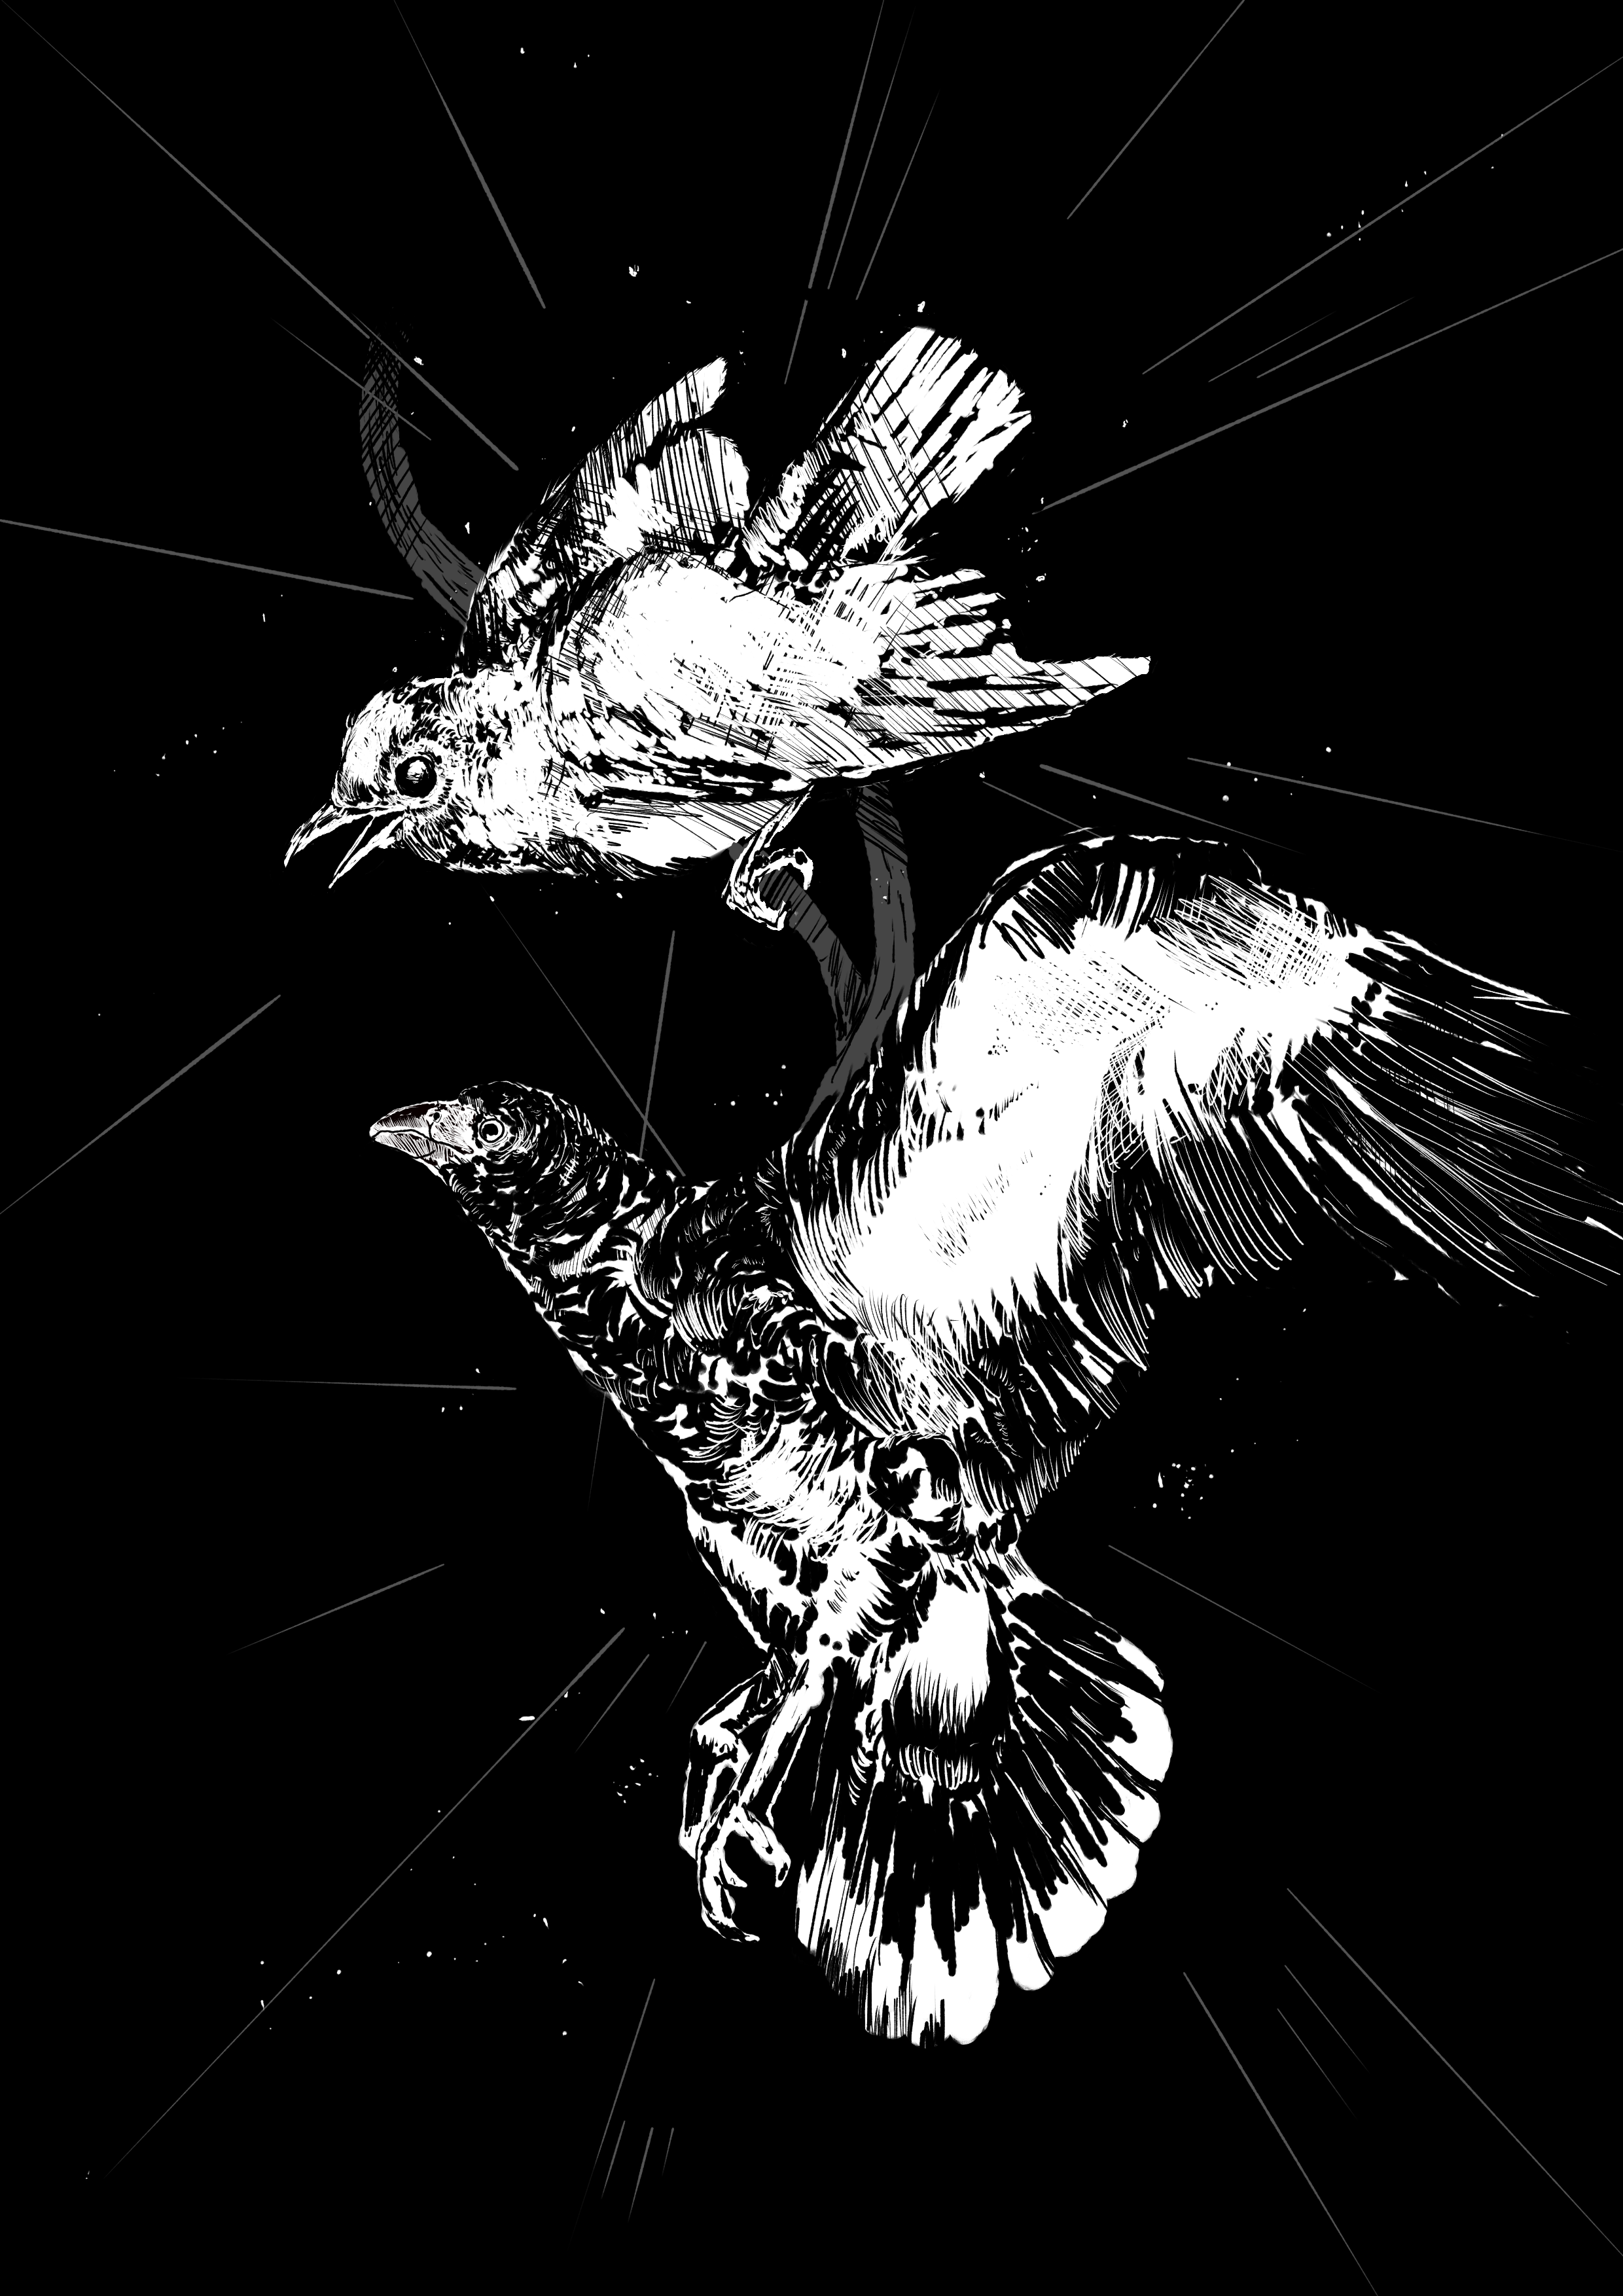
\includegraphics[width=0.6\paperwidth, scale=0.8]{Assets/alcaracrara.png}
    \endgroup
    \vspace*{\fill}
\end{center}        
\end{addmargin}
%*******************************************************
% Titlepage
%*******************************************************
\begin{titlepage}
    % if you want the titlepage to be centered, uncomment and fine-tune the line below (KOMA classes environment)
    \begin{addmargin}[-1cm]{-3cm}
    \begin{center}
        \large  

        \hfill

        \vfill

        \begingroup
            \color{mypurple}\spacedallcaps{\myTitle} \\ \bigskip
        \endgroup

        \spacedlowsmallcaps{\myName}

        \vfill

        
\includegraphics[width=6cm]{Assets/logo-ul.png} \\ \medskip

        \mySubtitle \\ \medskip   
        %\myDegree \\
        % \myDepartment \\                            
        \myFaculty \\
        \myUni \\ \bigskip

        \myTime\ -- \myVersion

        \vfill
        
        \end{center}


        \vspace{1em}
        {\large\textbf{Thesis Committee Composition:}}

        \begin{center}
        \vspace{1.5em}
        \begin{tabbing}
        \hspace{3cm} \= \hspace{5cm} \= \kill
        \textit{Chair :} \> \textit{To define} \\
        \\
        \textit{Reviewers :} \> XXX \textsc{XXX} \> University of XXX \\
        \> XXX \textsc{XXX} \> University of XXX \\
        \\
        \textit{Examiners :} \> XXX \textsc{XXX} \> University of XXXX \\
        \> XXX \textsc{XX} \> XXX \\
        \> XXX \textsc{XXX} \> XXX \\
        \\
        \textit{Supervisors :} \> Stephan \textsc{Merz} \> University of Lorraine (Primary Advisor) \\
        \> Gilles \textsc{Dowek} \> University of Paris-Saclay \\
        \end{tabbing}
        \end{center}
  \end{addmargin}
\end{titlepage}   
\thispagestyle{empty}

\hfill

\vfill

\noindent\myName: \textit{\myTitle,} \mySubtitle, %\myDegree, 
\textcopyright\ \myTime

\bigskip

\noindent\spacedlowsmallcaps{Supervisors}: \\
\mySupervisor \\
\myOtherSupervisor

\medskip

\noindent\spacedlowsmallcaps{Location}: \\
\myLocation

\medskip

\noindent\spacedlowsmallcaps{Time Frame}: \\
\myTime

\cleardoublepage%*******************************************************
% Dedication
%*******************************************************
\thispagestyle{empty}
%\phantomsection 
\refstepcounter{dummy}
\pdfbookmark[1]{Dedication}{Dedication}

\vspace*{3cm}

\begin{center}
    \emph{Ohana} means family. \\
    Family means nobody gets left behind, or forgotten. \\ \medskip
    --- Lilo \& Stitch    
\end{center}
%\cleardoublepage\include{FrontBackmatter/Foreword}
\cleardoublepage%*******************************************************
% Abstract
%*******************************************************
%\renewcommand{\abstractname}{Abstract}
\pdfbookmark[1]{Abstract}{Abstract}
\begingroup
\let\clearpage\relax
\let\cleardoublepage\relax
\let\cleardoublepage\relax

\chapter*{Abstract}
Powerful modern automated theorem provers (ATP) are increasingly used to establish the correctness of critical computer systems.
Among them, Satisfiability Modulo Theories (SMT) solvers play a central role thanks to their expressive power and efficiency in handling complex logical reasoning tasks.
However, their size and complexity make full formal verification of their implementations impractical, raising a fundamental question of trust:
\begin{center}
\emph{Can we trust the correctness of their results?}
\end{center}

A promising answer lies in \emph{proof logging}, where solvers produce proof traces that can be independently checked by simpler and verifiable proof checkers.
The Alethe format has recently emerged as a unified framework for representing such SMT proofs.
The Alethe format has been adopted by several SMT solvers for explaining why a set of constraints is unsatisfiable.
Yet, Alethe lacks a certified proof checker, limiting its adoption and trustworthiness.

In this thesis, we propose a reconstruction framework that translates Alethe proof traces into the Lambdapi proof assistant, an implementation of the $\lpm$-calculus modulo rewriting.
Lambdapi is a foundational proof assistant based on dependent type theory and rewriting rules, intended to serve as a pivot for exchanging proofs between interactive proof assistants.
We present a modular encoding of SMT logic and Alethe rules in Lambdapi, covering core theories such as propositional reasoning and linear arithmetic.

We detail the reconstruction process, including the elaboration of solver-specific simplifications, the reflective normalization of arithmetic expressions, and the handling of subproofs and quantified formulas.
Finally, we evaluate our implementation on benchmark examples and demonstrate that Alethe proofs generated by modern SMT solvers can be efficiently and reliably reconstructed in Lambdapi, paving the way toward portable and independently verifiable SMT proofs.

\endgroup			

\vfill
\cleardoublepage%*******************************************************
% Publications
%*******************************************************
\pdfbookmark[1]{Publications}{publications}
\chapter*{Publications}

% This might come in handy for PhD theses: some ideas and figures have appeared previously in the following publications:

\begin{refsection}[ownpubs]
    \small
    \nocite{*}
    \printbibliography[heading=none]
\end{refsection}
\cleardoublepage%*******************************************************
% Acknowledgments
%*******************************************************
\pdfbookmark[1]{Acknowledgments}{acknowledgments}

\begin{flushright}{\slshape    
    We have seen that computer programming is an art, \\ 
    because it applies accumulated knowledge to the world, \\ 
    because it requires skill and ingenuity, and especially \\
    because it produces objects of beauty.} \\ \medskip
    --- \defcitealias{knuth:1974}{Donald E. Knuth}\citetalias{knuth:1974} \citep{knuth:1974}
\end{flushright}



\bigskip

\begingroup
\let\clearpage\relax
\let\cleardoublepage\relax
\let\cleardoublepage\relax
\chapter*{Acknowledgments}
Put your acknowledgments here.

Many thanks to everybody who already sent me a postcard!

Regarding the typography and other help, many thanks go to Marco 
Kuhlmann, Philipp Lehman, Lothar Schlesier, Jim Young, Lorenzo 
Pantieri and Enrico Gregorio\footnote{Members of GuIT (Gruppo 
Italiano Utilizzatori di \TeX\ e \LaTeX )}, J\"org Sommer, 
Joachim K\"ostler, Daniel Gottschlag, Denis Aydin, Paride 
Legovini, Steffen Prochnow, Nicolas Repp, Hinrich Harms, 
 Roland Winkler, Jörg Weber, Henri Menke, Claus Lahiri, 
 Clemens Niederberger, Stefano Bragaglia, Jörn Hees, 
 and the whole \LaTeX-community for support, ideas and 
 some great software.

\bigskip

\noindent\emph{Regarding \mLyX}: The \mLyX\ port was intially done by 
\emph{Nicholas Mariette} in March 2009 and continued by 
\emph{Ivo Pletikosi\'c} in 2011. Thank you very much for your 
work and for the contributions to the original style.


\endgroup




\pagestyle{scrheadings}
\cleardoublepage%*******************************************************
% Table of Contents
%*******************************************************
%\phantomsection
\refstepcounter{dummy}
\pdfbookmark[1]{\contentsname}{tableofcontents}
\setcounter{tocdepth}{2} % <-- 2 includes up to subsections in the ToC
\setcounter{secnumdepth}{3} % <-- 3 numbers up to subsubsections
\manualmark
\markboth{\spacedlowsmallcaps{\contentsname}}{\spacedlowsmallcaps{\contentsname}}
\tableofcontents 
\automark[section]{chapter}
\renewcommand{\chaptermark}[1]{\markboth{\spacedlowsmallcaps{#1}}{\spacedlowsmallcaps{#1}}}
\renewcommand{\sectionmark}[1]{\markright{\thesection\enspace\spacedlowsmallcaps{#1}}}
%*******************************************************
% List of Figures and of the Tables
%*******************************************************
\clearpage



\begingroup 
    \let\clearpage\relax
    \let\cleardoublepage\relax
    \let\cleardoublepage\relax
    %*******************************************************
    % List of Figures
    %*******************************************************    
    %\phantomsection 
    \refstepcounter{dummy}
    %\addcontentsline{toc}{chapter}{\listfigurename}
    \pdfbookmark[1]{\listfigurename}{lof}
    \listoffigures

    \vspace{8ex}

    %*******************************************************
    % List of Tables
    %*******************************************************
    %\phantomsection 
    \refstepcounter{dummy}
    %\addcontentsline{toc}{chapter}{\listtablename}
    \pdfbookmark[1]{\listtablename}{lot}
    \listoftables
        
    \vspace{8ex}
%   \newpage
    
    %*******************************************************
    % List of Listings
    %*******************************************************     
    \renewcommand\lstlistlistingname{list of listings}

    
    % *******************************************************
    % ClassicThesis customization: List of Listings formatting
    % ------------------------------------------------------------
    % This block:
    %   • prefixes entries in \listoflistings by “Listing <n>”
    %   • removes the dotted leader between title and page number
    %   • keeps page numbers right-aligned
    % *******************************************************
    \makeatletter
    \@ifundefined{l@lstlisting}{}{%
    \let\l@lstlisting\l@listings
    }
    % Prefix before number
    \renewcommand{\cftlistingspresnum}{Listing~\scshape\MakeTextLowercase}

    % Remove dotted leaders and avoid large stretch
    \settowidth{\listingslabelwidth}{\cftlistingspresnum~999}
    \makeatother
    %*******************************************************
 
   \refstepcounter{dummy}
    %\addcontentsline{toc}{chapter}{\lstlistlistingname}
    \pdfbookmark[1]{\lstlistlistingname}{lol}
    \listoflistings

    \vspace{8ex}
       
    %*******************************************************
    % Acronyms
    %*******************************************************
    %\phantomsection 
    \refstepcounter{dummy}
    \pdfbookmark[1]{Acronyms}{acronyms}
    \markboth{\spacedlowsmallcaps{Acronyms}}{\spacedlowsmallcaps{Acronyms}}
    \chapter*{Acronyms}
    \begin{acronym}[ATPX]
        \acro{SMT}{Satisfiability Modulo Theories}
        \acro{ATP}{Automated Theorem Proving}
        \acro{AR}{automated Reasoning}
        \acro{SAT}{Boolean Satisfiability Problem}
        \acro{AC}{Associative Commutative}
    \end{acronym}                     
\endgroup




%*******************************************************
% Mainmatter
%*******************************************************
\cleardoublepage\pagenumbering{arabic}

\cleardoublepage

\part{Context}

%************************************************
\chapter{Introduction}\label{ch:introduction}
%************************************************

Satisfiability Modulo Theories (SMT) solvers \cite{cvc5,verit} are automated reasoning (AR) tools that have become essential in a wide range of formal reasoning tasks, including program verification and interactive theorem proving.
Their efficiency and expressive power enable them to handle complex logical proofs and verifications with speed.
At the same time, the growing reliance on SMT solvers raises a fundamental question of trust: \textit{can we be confident that the results produced by these highly complex SMT solvers are correct?}

Despite their central role, SMT solvers are large software systems with complex architectures \cite{cvc5}, often comprising hundreds of thousands of lines of code.
This complexity makes it extremely difficult to guarantee their correctness.
The annual SMT-COMP competition \cite{smtcomp2015–2018,SMT-COMP}, regularly uncovers cases where different solvers disagree on the satisfiability status of the same benchmark.
State-of-the-art SMT solvers have been found to have bugs \cite{bugsmt} due in part to error-prone optimizations, despite the best efforts of developers.
Such discrepancies highlight the practical risk of relying blindly on solver outputs in safety critical applications.

A natural response to this problem is to attempt the certification of the solver itself.
However, formally verifying such a large and complex codebase is highly impractical \cite[\S 2.2.1]{formal-method-book}.
Simplifying a solver’s design to ease certification would necessarily come at the expense of performance, which is a key factor in their adoption.
Moreover, certification tends to ``freeze'' the implementation: once a system is verified, the integration of new features, heuristics, or optimizations becomes prohibitively costly, since each change would require a new certification effort.
Consequently, directly certifying solvers in a late lifecycle of development might not scale with the pace of their development.

A first alternative is to develop a certified solver in a proof assistant environment such as the IsaSAT solver \cite{fleury:tel-02963301,fleury:hal-01904647} that is a fully verified SAT solver developed in Isabelle/HOL \cite{isabelle-hol-ref}.
This alternative offers strong guarantees about the correctness of the implementation itself, since the solver is extracted from a machine-checked formalization.
Moreover, it has been demonstrated to achieve competitive performance in SAT solving \cite{EDA-challenge}.
While IsaSAT has been extended to output DRAT proofs, these proofs are not yet checked within the verified framework, and therefore do not provide the same level of end-to-end certification as approaches that combine solver output with independently verified proof checking.
In this respect, IsaSAT advances the state of the art by providing a verified implementation of SAT solving.
However, it does not yet close the gap toward fully certifying solver results.
Moreover, the restriction to SAT limits its applicability in domains where SMT theories reasoning is required.


A second alternative line of research is the \emph{proof logging} \cite{proof-logging}, where the approach is to certify the \emph{results} rather than the solver implementation.
The proof logging is a technique for automatically reviewing the reasoning steps of a proof engine by a separate tool.
This is achieved by requiring the solver to produce a proof, or certificate, of its output.
An SMT proof formally records the logical reasoning that leads to a solution, enabling independent verification by a separate proof checker.
Essentially, the task of proof checking is conceptually simpler and typically much faster than solving itself.
Moreover, a well designed trace format allows traces to be generated and checked with low performance overhead.
This decouples the trust in solver results from the correctness of the solver’s implementation, thereby providing a more practical path toward trustworthy automated reasoning.
It is then the checker of the proof trace that becomes the critical link for establishing confidence in the correctness of a verdict, and establishing soundness of a proof checker is much easier than verifying an SMT solver.
An attractive way of building and verifying a trace checker is to have a proof assistant interpret a trace and produce a proof that is accepted by the kernel of the proof assistant.
This method is known as \emph{proof reconstruction} \cite{z3recon}.
For example, this approach has been adopted in several proof assistants that employ \emph{hammers} for discharging goals to automatic theorem provers (ATPs), including SMT solvers.
Examples include Sledgehammer \cite{Sledgehammer} for Isabelle/HOL and CoqHammer \cite{coqhammer1,coqhammer2} for Coq.
The hammer translates the conjecture and facts supplied by the user or harvested from the context to the input language of the back-end, invokes it, and, in the case of success, attempts to reconstruct the proof in the logic of the proof assistant, based on a trace of the proof found by the back-end.

Alethe is an established SMT proof format generated by the solvers veriT \cite{verit} and cvc5 \cite{cvc5}.
As the example \cref{lst:alethe-ex-intro} shows the format is close to SMT-LIB and allows both coarse and fine-grained steps, facilitating proof production.
However, it lacks a stand-alone checker, which harms its usability and hinders its adoption. 
Moreover, the coarse-grained steps can be too expensive to check and lead to verification failures.

\lstinputlisting[language=SMT]{Assets/example_uf.smt2}
\begin{center}
$\lightning$
\end{center}
\lstinputlisting[language=SMT,label={lst:alethe-ex-intro},caption={An SMT problem and its Alethe proof found by cvc5.}]{Assets/example_uf.proof}


\begin{figure}[b]
    \centering
    \begin{tikzpicture}
      \path (0,0) node (lp) {\textcolor{red}{Lambdapi}}
            (-4,1) node (coq) {Coq}
            (-3,2) node (lean) {Lean}
            (0,2) node [draw, dashed, purple] (smt) {\color{purple}\textbf{Alethe}}
            (4,2) node (isa) {Isabelle}
            (4,0) node (agda) {Agda}
            (-3,-2) node (k) {$\mathbb{K}$-framework}
            (0,-3) node (mat) {Matita}
            (2,-2) node (hol) {HOL}
            (-4,-1) node (pvs) {PVS}
            (4,-1) node (ze) {Zenon \& ArchSAT}
            ;
      \draw[->,red, thick] (smt) -- (lp) node[midway,sloped,above] {};
      \draw[->] (lean) -- (lp) node[midway,sloped,above] {\footnotesize{lean2dk}};
      \draw[->] (isa) -- (lp) node[midway,sloped,above] {\footnotesize{isabelle\_dk}};
      \draw[->] (agda) -- (lp) node[midway,sloped,above] {\footnotesize{agda2dk}};
      \draw[<->] (ze) -- (lp) node[midway,sloped,above] {};
      \draw[<->] (hol) -- (lp) node[midway,sloped,above] {\footnotesize{hol2dk}};
      \draw[<->] (mat) -- (lp) node[midway,sloped,above] {\footnotesize{Krajono}};
      \draw[->] (pvs) -- (lp);
      \draw[->] (k) -- (lp) node[midway,sloped,above] {\footnotesize{KaMeLo}};
      \draw[<->] (coq) -- (lp)  node[midway,sloped,above] {\footnotesize{vodk}};
    \end{tikzpicture}
    \caption{Lambdapi, an assembly language for proof systems.}
    \label{fig:interop-intro}
\end{figure}

This thesis addresses these challenges by introducing a translation framework from Alethe proofs to Lambdapi, a proof assistant for the $\lp$-calculus modulo rewriting ($\lpm$).
The $\lpm$-calculus combines dependent types, which enable precise encodings of object logics, with modulo theory which extends reasoning by allowing rewrite rules for defining theories and deductions.
In this way, the $\lpm$-calculus provides a meta-logic capable of expressing object logics, axioms, inference rules, and proofs of various theorem provers.
Lambdapi also supports exporting proofs to other systems (\cref{fig:interop-intro}), providing a bidirectional connection between different proof environments.
This has been one of the principal reasons for selecting Lambdapi, since it enables the conversion and sharing of Alethe proofs with other logical systems such as Rocq and Isabelle/HOL.

In this work, we identified common challenges and developed general encoding strategies.
Based on these strategies, we present a modular encoding in Lambdapi of selected Alethe inference rules.
We then empirically evaluate the effectiveness of this approach through the automated generation of proof certificates verifiable within the Lambdapi proof assistant.

\section{Thesis outline}
\label{sec:thesis-outline}

This chapter has introduced the challenges of ensuring trustworthiness in SMT solvers, highlighting the need for verifiable proofs to address the complexity and potential incorrectness of SMT solvers.
While SMT solvers are widely used in formal methods, their outputs are often taken for granted, despite the risks of errors in large, optimized codebases.
The goal of this thesis is to provide a robust framework for certifying SMT proofs by translating them into a dependently typed setting, making them both trustworthy and portable across different proof assistants.
The thesis is structured as follows:

\begin{itemize}
\item In \cref{ch:intro-lambdapi}, we introduce Lambdapi, the foundational framework for our work.
    We present the $\lambda\Pi$-calculus modulo rewriting, its typing system, and key features, including rewrite rules and inductive types.
    This chapter establishes the formal basis for encoding SMT proofs.
    It demonstrates why Lambdapi is uniquely suited for this task due to its interoperability with other proof assistants and its support for user-defined rewriting.

\item In \cref{ch:smt}, we provide background on Satisfiability Modulo Theories (SMT), covering the SMT-LIB standard, the semantics of first-order logic with theories, and the architecture of modern SMT solvers.
We discuss the role of proof production in ensuring solver correctness and motivate the need for a standardized, verifiable proof format like Alethe.

\item In \cref{ch:alethe}, we dive into the Alethe proof format, detailing its design, syntax, and logical rule system including resolution, quantifier instantiation, and theory specific rules (e.g., for linear arithmetic).
We explain how Alethe represents proofs as sequences of steps.
This chapter also highlights the challenges posed by coarse-grained proof steps and the lack of a standalone checker, which our work addresses.

\item In \cref{ch:elab}, we describe how preprocessing tools, such as Carcara \cite{carcara} and RARE \cite{rare}, refine and elaborate proofs before translation, eliminating redundant steps and preparing them for reconstruction in Lambdapi.

\item In \cref{ch:relatedworks}, we survey related work, comparing Alethe with other proof formats (e.g., Eunoia) and discussing existing approaches to integrating SMT solvers with proof assistants.
    We position our work within the broader landscape of proof certification for smt solver.

\item In \cref{ch:encoding}, we lay the groundwork for our encoding by defining how SMT logic can be represented in Lambdapi.
    We develop a prelude that captures SMT-LIB's sorts, terms, and formulas, and show how to encode theories like Linear Integer Arithmetic (LIA) and Linear Arithmetic (LA).
    This chapter bridges the gap between SMT's many-sorted first-order logic and Lambdapi's dependent types.

\item In \Cref{ch:reconstruction}, \ref{ch:reconstruction-ul} and \ref{ch:reconstruction-la}, we present the core of our reconstruction methodology.
    The \cref{ch:reconstruction-ul} focuses on reconstructing first-order proofs, including tautologies, resolution, and quantifier handling, while \cref{ch:reconstruction-la} extends this to linear arithmetic proofs.
    We introduce reflective techniques for normalizing arithmetic expressions and prove the correctness of our translations, ensuring that reconstructed proofs faithfully represent the original SMT reasoning.

\item In \cref{ch:soundness}, we formalize the correctness of our translation, proving that the encoding preserves semantic entailment.
    This chapter provides the theoretical guarantees that underpin our approach.

\item In \cref{ch:evaluation}, we shift to practical evaluation, presenting benchmarks and case studies that demonstrate the efficiency and scalability of our method.
    We show how our toolchain can validate proofs from real-world applications, including TLAPS proofs \cite{tla-proofs}, and discuss optimizations for parallel checking.

\item Finally, in Chapter~\cref{ch:conclusion}, we conclude by summarizing our contributions and discussing limitations and future directions.
    We highlight the potential for extending our work to additional theories (e.g., bit-vectors) and integrating with more proof assistants, ultimately aiming to establish Alethe as a standard for proof exchange in formal methods.
\end{itemize}


%*****************************************
\chapter{Related Works}\label{ch:relatedworks}
%*****************************************

\section{The proof assistant TLAPS}

\subsection{The language}

\tlaplus is a specification language based on the Temporal Logic of Actions and Zermelo–Fraenkel set theory with the Axiom of Choice (ZFC) \cite{tlabook,tla-ref}.
It is particularly used for specifying concurrent and distributed systems.
The \tlaplus Proof System (TLAPS) extends the language with a formal proof syntax and a tactical proof language \cite{tla-proofs}.

TLAPS includes a \emph{Proof Manager} that decomposes proofs into individual proof obligations, which are then dispatched to various backend provers.
These currently include Isabelle/\tlaplus \cite{isabelle-hol-ref}, Zenon \cite{zenonmodulo},
the SMT solvers cvc5 \cite{cvc5}, veriT \cite{verit} and Z3 \cite{z3}, and finally the LS4 prover for temporal logic.
Each obligation is translated into the logic supported by the corresponding backend.
For SMT solvers \cite{new-encoding-tlaps}, the supported logics include \textbf{UF}, \textbf{LIA}, and \textbf{NIA}.
At present, TLAPS does not verify the correctness of solver outputs, except in the case of Zenon, whose proofs can be independently validated by Isabelle,
and in the case of Isabelle/\tlaplus backend.

As the \cref{fig:interop-tla} suggests, the previous work discussed in \cref{ch:reconstruction} can be leveraged to verify \tlaplus proofs from the SMT solver backend.
The proposed approach involves extracting the output generated by the SMT backend, retrieving the corresponding proof from cvc5 or veriT, and reconstructing it within Lambdapi to establish its validity.


\subsection{Validating TLAPS proof}
\label{sec:validating-tlaps-proof}

% -------------- MODULE Cantor1 -----------------
% THEOREM cantor ==
%   \A S :
%     \A f \in [S -> SUBSET S] :
%       \E A \in SUBSET S :
%         \A x \in S :
%           f [x] # A
% PROOF
%   <1>1. TAKE S
%   <1>2. TAKE f \in [S -> SUBSET S]
%   <1>3. DEFINE T == { z \in S : z \notin f[z] }
%   <1>4. WITNESS T \in SUBSET S
%   <1>5. TAKE x \in S
%   <1>6. QED BY x \in T \/ x \notin T
\begin{figure}[tb]
\centering
\begin{nomodule}
\topbar{Cantor}
\[\begin{noj}
  \THEOREM\ cantor\ \deq \\
  \A S : \\
  \quad \A f \in [S \implies \SUBSET\ S] : \\
  \quad\quad \exists A \in \SUBSET\ S : \\
  \quad\quad\quad \forall x \in S : \\
  \quad\quad\quad\quad f \sq{x}{} \mathbin{\#} A \\
  \ps{1}{1.}\ \TAKE\ S \\
  \ps{1}{2.}\ \TAKE\ f \in [S \implies \SUBSET\ S]\\
  \ps{1}{3.}\ \DEFINE\ T\ \deq\ \{ z \in S : z \notin f[z] \}\\
  \ps{1}{4.}\ \WITNESS\ T\ \in \SUBSET\ S \\
  \ps{1}{5.}\ \TAKE\ x \in S \\
  \ps{1}{6.}\ \QED\ \BY\ x \in T \lor x \notin T
\end{noj}\]
\bottombar
\end{nomodule}
\caption{Cantor theorem in \tlaplus}
\label{fig:cantor-tlaps}
\end{figure}

\tlaplus proofs are hierarchically structured and are generally written topdown.
The assertion that the cantor theorem stating that no function ($f$) from a set ($S$) to its power set (\SUBSET\ $S$) can be surjective is formalized in \tlaplus as the theorem in \cref{fig:cantor-tlaps}.
Each proof in the hierarchy ends with a \QED\ step that asserts the proof's goal.
Proofs are incrementally decomposed into simpler subproofs across multiple levels. Each proof consists of labeled steps $\ps{i}{k.}$, that reflect their depth in the proof tree, where level $n$ indicates the nesting depth.
Steps may introduce assumptions, intermediate claims, or invoke previously proven results, using TLAPS tactics such as \ASSUME/\PROVE\, \TAKE\ or \WITNESS.
The proof is completed when the root goal is reduced to a collection of leaf obligations marked as \QED\ and discharged by backend provers.
Besides, TLAPS does not yet handle temporal reasoning.

For each step $\ps{i}{k.}$ in \tlaplus proof, there is a proof obligation that is to be proved.
The obligation contains a context of known facts, definitions, declarations, and a goal.
Obligations are sent to a suitable backend select by the PM (Zenon, Isabelle/TLA, SMT solvers) that tries to prove it.
In the case of \cref{fig:cantor-tlaps}, we will have 6 proof obligations $(\ps{1}{1.} - \ps{1}{6.})$ that will be discharged to the backend.
For example, the proof obligation relative to the final step $\ps{1}{6.}$ is given as follows:

% ===============================================


% ;;	ASSUME NEW CONSTANT CONSTANT_S_,
% ;;	       NEW CONSTANT CONSTANT_f_ \in [CONSTANT_S_ -> SUBSET CONSTANT_S_],
% ;;	       NEW CONSTANT CONSTANT_x_ \in CONSTANT_S_,
% ;;	       CONSTANT_x_
% ;;	       \in {CONSTANT_z_ \in CONSTANT_S_ :
% ;;	              CONSTANT_z_ \notin CONSTANT_f_[CONSTANT_z_]}
% ;;	       \/ CONSTANT_x_
% ;;	          \notin {CONSTANT_z_ \in CONSTANT_S_ :
% ;;	                    CONSTANT_z_ \notin CONSTANT_f_[CONSTANT_z_]} 
% ;;	PROVE  CONSTANT_f_[CONSTANT_x_]
% ;;	       # {CONSTANT_z_ \in CONSTANT_S_ :
% ;;	            CONSTANT_z_ \notin CONSTANT_f_[CONSTANT_z_]}
\begin{figure}[tb]
\centering
\[\begin{noj}
  \quad\begin{noj2}
    \ASSUME & \NEW\ \CONSTANT\ S, \\
            & \NEW\ \CONSTANT\ f  \in [ S \implies \SUBSET\ S ], \\
            & \NEW\ \CONSTANT\ X  \in S, \\
            & \quad X \in T \lor \quad X \notin T \\
    \PROVE  & f[X] \neq T
  \end{noj2}
\end{noj}\]
\caption{Proof obligation of step  $\ps{1}{6.}$}
\label{fig:cantor-po}
\end{figure}

It assumes an arbitrary set $S$, a function $f \in [S \implies \SUBSET\ S]$, and an arbitrary element $X \in S$.
The goal is to prove that $f[X] \neq \{ z \in S \mid z \notin f[z] \}$.
This corresponds to the diagonalization step: given the definition $T \deq \{ z \in S \mid z \notin f[z] \}$ from $\ps{1}{3.}$, we aim to show that $T$ is not in the image of $f$.
To this end, we must show that for any $X \in S$, $f[X] \neq T$.
The assumption $X \in T \lor X \notin T$ provides a complete case split, and in either case, the assumption $f[X] = T$ leads to a contradiction, which suffices to discharge the proof obligation.

There would be 4 proofs obligations that will be cover by the SMT solvers, and 2 by Zenon for the most simple one. 
The SMT backend of \tlaplus generated the corresponding SMT input problem presented in \cref{lst:cantor-smt}.
We use the \textit{Cantor} example to illustrate the general approach taken to encode set-theoretic reasoning, as all proof obligations produced by the backend follow a similar structure.
Full details of the SMT encoding for \tlaplus are provided in \cite{new-encoding-tlaps}.
Since \tlaplus is based on ZFC that does not include \emph{sort}, the backend introduces a universal uninterpreted sort \tt{Idv} (line 2) to represent the domain of all values.
Within this setting, the function symbol \tt{FunApp} (line 6) encodes function application (i.e. $f[x]$), while \tt{Mem} (line 7) denotes set membership ($\in$).
The declared constant symbols \tt{S} and \tt{f} correspond to the set $S$ and function $f$ in the original proof.
The auxiliary function \tt{SetSt\_flatnd\_1} defines the diagonal set $T = \{ z \in S \mid z \notin f[z] \}$ by comprehension; this is specified by a universally quantified axiom stating that an element $X$ belongs to \tt{SetSt\_flatnd\_1 A} if and only if $X \in A$ and $X \notin f[X]$.
This axiom captures the definition of $T$ in a first-order setting.
The disjunctive assertion \tt{(or (Mem x ...) (not (Mem x ...)))} encodes a \emph{classical} reasoning by cases over whether $x$ belongs to $T$, reflecting how the proof splits based on $x \in T$ or $x \notin T$ in the original \tlaplus argument. 
Finally, the goal is asserted as the negation of the equation \tt{(FunApp f x) = (SetSt\_flatnd\_1 S)}, encoded via a triggerable equality predicate \tt{TrigEq\_Idv}.
Triggers play a crucial role in optimizing the encoding, as discussed in \cite[\S3]{new-encoding-tlaps}.
This encoding faithfully mirrors the structure of the original \tlaplus proof obligation \cref{fig:cantor-po}.

\smallskip

\begin{lstlisting}[language=SMT, caption={Proof obligation of step $\ps{1}{6.}$ in Cantor theorem},label={lst:cantor-smt}]
;; Sorts
(declare-sort Idv 0)

;; Hypotheses

(declare-fun FunApp (Idv Idv) Idv)
(declare-fun Mem (Idv Idv) Bool)
(declare-fun TrigEq_Idv (Idv Idv) Bool)
...
(declare-fun S () Idv)
(declare-fun f () Idv)
(declare-fun SetSt_flatnd_1 (Idv) Idv)

;; Axiom: SetStDef SetSt_flatnd_1
(assert
  (!
    (forall ((a Idv) (x Idv))
      (!
        (= (Mem x (SetSt_flatnd_1 a))
          (and (Mem x a)
            (not
              (Mem x
                (FunApp CONSTANT_f_ x)))))
        :pattern ((Mem x (SetSt_flatnd_1 a)))
        :pattern ((Mem x a)
                   (SetSt_flatnd_1 a))))
    :named |SetStDef SetSt_flatnd_1|))

(assert (forall ((A Idv) (X Idv))
        ( = 
            (Mem X (SetSt_flatnd_1 A))
            (and (Mem X A) (not (Mem X (FunApp f X))))
        )
    )
)

;; Goal
(assert (! (not (not (TrigEq_Idv (FunApp f x_) (SetSt_flatnd_1 S)))) :named |Goal|))
\end{lstlisting}

\smallskip

%*****************************************
\chapter{Lambdapi}\label{ch:intro-lambdapi}
%*****************************************

\section{The \texorpdfstring{\lp}-Calculus modulo}

The \lp-calculus modulo rewriting (\lpm)  extends the Edinburgh Logical Framework (LF) \cite{lf} by allowing user-defined rewrite rules at both the term and type levels.
In this framework, all terms and types are identified modulo the congruence relation generated by standard $\beta$-reduction together with the specified rewrite rules.
{\lpm} is implemented in the Lambdapi proof language \cite{lambdapi}. Lambdapi, a successor of the Dedukti proof language \cite{Dedukti-ref, Dedukti-ref2}, is an implementation of {\lpm}; it differs primarily by offering an integrated proof tactic language.
However, it can still import and export Dedukti theories to maintain compatibility. Lambdapi, similarly to Dedukti, is designed to facilitate the exchange of proofs between systems.
Lambdapi/Dedukti was used to translate \cite{thire:tel-03224039} the Matita arithmetic library to several systems, including Coq and PVS, export \cite{blanqui:hal-04613926} the HOL Light standard library to Coq,
and verifying Event-B proof \cite{eventb2lp}.

% \section{An assembly for proof assistant}

\begin{figure}[t]
    \centering
    \begin{tikzpicture}
      \path (0,0) node (lp) {\begin{tabular}{c}
        \textcolor{red}{Lambdapi} \\
        \hline
        \textcolor{red}{Dedukti}
      \end{tabular}}
            (-4,1) node (coq) {Coq}
            (-3,2) node (lean) {Lean}
            % (0,2) node [draw, dashed, purple] (smt) {\color{purple}\textbf{SMT}}
            (4,2) node (isa) {Isabelle}
            (4,0) node (agda) {Agda}
            (-3,-2) node (k) {$\mathbb{K}$-framework}
            (0,-3) node (mat) {Matita}
            (2,-2) node (hol) {HOL}
            (-4,-1) node (pvs) {PVS}
            (4,-1) node (ze) {Zenon \& ArchSAT}
            ;
      % \draw[->,red, thick] (smt) -- (lp) node[midway,sloped,above]
      % {\footnotesize{Carcara}};
      \draw[->] (lean) -- (lp) node[midway,sloped,above] {\footnotesize{lean2dk}};
      \draw[->] (isa) -- (lp) node[midway,sloped,above] {\footnotesize{isabelle\_dk}};
      \draw[->] (agda) -- (lp) node[midway,sloped,above] {\footnotesize{agda2dk}};
      \draw[<->] (ze) -- (lp) node[midway,sloped,above] {};
      \draw[<->] (hol) -- (lp) node[midway,sloped,above] {\footnotesize{hol2dk}};
      \draw[<->] (mat) -- (lp) node[midway,sloped,above] {\footnotesize{Krajono}};
      \draw[->] (pvs) -- (lp);
      \draw[->] (k) -- (lp) node[midway,sloped,above] {\footnotesize{KaMeLo}};
      \draw[<->] (coq) -- (lp)  node[midway,sloped,above] {\footnotesize{vodk}};
    \end{tikzpicture}
    \caption{Lambdapi, an assembly language for proof systems.}
    \label{fig:interop}
\end{figure}

\section{Signature rules}

We start by defining the basic elements of the \lpm{} calculus and giving their syntax.
The terms of the \lp-Calculus Modulo are the same as in \lp-Calculus (LF).
The Terms of \lpm{} are divided into three levels: Objects (denoted by $M$ and $N$), Types (denoted by $A$ and $B$), and Kinds (denoted by $K$).
The syntax of \lpm{} is given by the following grammar:


\begin{flalign*}
&\text{Objects}  & M, N  &::= c \pipe x \pipe \lambda\,x : A, M \mathrel{|} M~N &\\
&\text{Types}   & A,B &::= a \pipe \Pi\,x:A, B \pipe A~M &\\
&\text{Kinds} & K & ::= \type \pipe \Pi\,x:A, K &\\
&\text{Terms} & t,u & ::= M \pipe A \pipe K \pipe \kind  &
\end{flalign*}

Where $c$ is a constant and $x$ is a variable  (ranging over disjoint sets).
Dependent products  $\Pi\,x : A.\,B$ (respectively $\Pi\,x : A.\,K$) are simply written $A \rightarrow B$ when $x$ does not occur in $B$ (respectively $K$), $\lambda\,x : A.\,M$ is an abstraction, and  $M~N$ (respectively $A~M$) is an application.

\begin{definition}[Substitutions]
A substitution $\sigma$ is a function written \([ x_1 \leftarrow N_1, \dots, x_n \leftarrow N_n]\), from the set of variables to the set of terms with a finite domain.
We write $t\sigma$ the term $t$ where the variables are replaced by their image by $\sigma$.
\end{definition}

Contexts $\Gamma$ is a finite sequence used to specify the type of the free variables.
Signatures (denoted $\Sigma$) serve as the \emph{global context} and are used to declare the constants and rewrite rules considered by the users.

\begin{flalign*}
&\text{Contexts}  & \Gamma  &::= \langle\rangle \pipe \Gamma,x: A &\\
&\text{Signature} & \Sigma &::= \langle\rangle \pipe \Sigma, c: A \pipe \Sigma, a: K \pipe \Sigma, M \re N \pipe \Sigma,A \re B &
\end{flalign*}

A \emph{signature} \index{$\Sigma$} is a finite sequence of \emph{assumptions} $c : A$ (respectively $c:K$), indicating that constant $c$ is of type $C$ (respectively kind $K$), \emph{definitions} $c := A : M$, indicating that $c$ has the value $M$ and type $A$.
We write $\langle\rangle$ when contexts or signatures are empty. Rewrite rules are pairs $M \re N$ (respectively $A \re B$), where the head symbol of $M$ (respectively $A$) is a constant
and where free variables of $N$ (respectively $B$) occur in M (respectively $A$). The rewrite rules must preserve typing, i.e., whenever $\Gamma \vdash_\Sigma t\sigma: A$ with any substitution $\sigma$, and $t \longrightarrow_{\beta\Sigma} v$ then $\Gamma \vdash_\Sigma v\sigma: A$.


\section{Rewriting}

In the \lpm-Calculus we distinguish two kinds of rewriting.

\subsection{\texorpdfstring{$\beta$}{}-reduction}

The first kind of rewriting is $\beta$-reduction, which is defined as usual.

\begin{definition}[$\beta$-reduction] The $\beta$-reduction relation $\longrightarrow_\beta$ is the smallest relation on terms containing
\( (\lambda x:A, u)v \longrightarrow_\beta u[x \leftarrow v] \) for any $A$, $u$ and $v$ and closed by subterm reduction.
\end{definition}

\begin{notation}
We write $\longrightarrow^*_\beta$ for the reflexive and transitive closure of $\longrightarrow_\beta$ and $\equiv_\beta$ for the congruence generated by $\longrightarrow_\beta$.
\end{notation}

\subsection{\texorpdfstring{$\Sigma$}{}-reduction}

The second kind of rewriting is $\Sigma$-reduction, the relation generated by the rewrite rules of a global context $\Sigma$.

\begin{definition}[$\Sigma$-reduction]
Let $\Sigma$ be a global context. The  $\Sigma$-reduction relation $\longrightarrow_\Sigma$ is the smallest relation on terms containing $u \longrightarrow_\Sigma v$
for each rule $u \re v \in \Sigma$ and closed by substitution and subterm reduction.
\end{definition}

\begin{notation}
We write:

\begin{itemize}
\item $\longrightarrow^*_{\Sigma}$ the reflexive and transitive closure of $\longrightarrow_\Sigma$;
\item $\equiv_\Sigma$ the congruence generated by $\longrightarrow_{\Sigma}$;
\item $\longrightarrow_{\beta\Sigma}$ for $\longrightarrow_{\beta} \cup \longrightarrow_{\Sigma}$;
\item $\longrightarrow^*_{\beta\Sigma}$ the reflexive and transitive closure of $\longrightarrow_{\beta\Sigma}$;
\item $\equivL$ for the equivalence relation generated by $\longrightarrow_{\beta\Sigma}$.
\end{itemize}
\end{notation}

Lambdapi implements untyped rewriting because it will be inefficient to check the well-typedness of the substitution at each reduction step.

\begin{definition}[Linearity]
We also define the properties:
\begin{itemize}
\item A term is linear if no variable occurs twice in it;
\item A rewrite rule $M \re N$ is left-linear if $M$ is linear.
\end{itemize}
\end{definition}

\begin{example}[Non-linear rule]
The rule $\kw{C}~x~x~y\re u$ is non-(left-)linear because the variable $x$ occurs twice on the left of the arrow.
\end{example}

\section{Typing system}
\label{sect:lambdapi}

We now give the typing rules of the \lpm{}-Calculus in \cref{fig:lp-typing-rules}.
A Lambdapi typing judgment $\Gamma \vdash_\Sigma t : A$ asserts that term $t$ has type $A$ in the context $\Gamma$ and the signature $\Sigma$.


\begin{definition}[Well-Typed Term]
We say that a term $t$ has a type $A$ in global context $\Sigma$ and local context $\Gamma$ if the judgment $\Sigma,\Gamma \vdash t: A$ is
derivable by the inference rules of \cref{fig:lp-typing-rules}. We say that a term is well-typed if such an $A$ exists.
\end{definition}

\begin{definition}[Well-Formed Local Context]
A local context $\Gamma$ is well-formed with respect to a global context $\Sigma$ if the judgment $\Sigma \vdash \Gamma$ is derivable by the inference rules of \cref{fig:lp-typing-rules}.
\end{definition}


\begin{figure}
  \[
    \begin{prooftree}
      \infer0[(Empty)]{ \vdash_\Sigma \langle\,\rangle  }
    \end{prooftree}
    \qquad
    \begin{prooftree}
      \hypo{ \vdash_\Sigma \Gamma }
      \hypo{ \Gamma \vdash_\Sigma A : s }
      \infer2[(Decl) $x \notin \Gamma$]{ \vdash_\Sigma \Gamma, x : A  }
    \end{prooftree}
  \]
  \medskip
  \begin{center}
    \begin{prooftree}
    \hypo{ \vdash_\Sigma \Gamma }
    \hypo{\Gamma \vdash_\Sigma A : s}
    \infer2[(Const)]{ \Gamma \vdash_\Sigma c : A }
    \end{prooftree}
  \end{center}
  \medskip
  \[
    \begin{prooftree}
      \hypo{ \vdash_\Sigma \Gamma }
      \infer1[(Sort)]{ \Gamma \vdash_\Sigma \type : \kind }
    \end{prooftree}
    \qquad
    \begin{prooftree}
      \hypo{ \vdash_\Sigma \Gamma }
      \infer1[(Var) $x : A \in \Sigma$]{ \Gamma \vdash_\Sigma x : A }
    \end{prooftree}
  \]
  \medskip
  \begin{center}
    \begin{prooftree}
    \hypo{\Gamma, \vdash_\Sigma A : \type }
    \hypo{\Gamma, x: A \vdash_\Sigma B: s}
    \hypo{\Gamma, x : A \vdash_\Sigma t: B}
    \infer3[(Abs)]{ \Gamma \vdash_\Sigma \lambda x: A, t : \Pi x : A, B }
    \end{prooftree}
  \end{center}

  \begin{center}
    \begin{prooftree}
      \hypo{ \Gamma \vdash_\Sigma A : \type }
      \hypo{ \Gamma, x : A \vdash_\Sigma B : s }
      \infer2[(Prod)]{ \Gamma \vdash_\Sigma \Pi x : A, B : s }
    \end{prooftree}
    \quad
  \end{center}

  \medskip

  \begin{center}
    \begin{prooftree}
      \hypo{ \Gamma \vdash t : \Pi x : A, B }
      \hypo{ \Gamma \vdash  u : A }
      \infer2[(App)]{ \Gamma \vdash_\Sigma t~u : B[u \leftarrow x] }
    \end{prooftree}
  \end{center}

  \medskip

  \begin{center}
  \begin{prooftree}
  \hypo{\Gamma, \vdash_\Sigma B: u}
  \hypo{\Gamma \vdash_\Sigma t: A}
  \hypo{A \textcolor{red}{\equiv_{\beta\Sigma}} B}
  \infer3[(Conv)]{ \Gamma \vdash_\Sigma t: B }
  \end{prooftree}
  \end{center}
  \caption{Typing rules of \lpm}
  \label{fig:lp-typing-rules}
  \end{figure}

\begin{remark}
The typing rules shown in \cref{fig:lp-typing-rules} are similar to those of  \lp{}-Calculus \cite[\S 2]{lf}, except for the additional rule (Conv) that identifies types modulo $\equivL$ instead of just modulo $\equiv_\beta$.
\end{remark}

Besides the new conversion relation, the main difference between the \lp-Calculus and the \lpm-Calculus is the presence of the rewrite rules
in global contexts. We need to take this into account when typing global contexts. A key feature of any type system is the preservation of typing by reduction: the
subject reduction property.

\begin{definition}[Subject Reduction]
Let $\longrightarrow_r$ be a binary relation on terms.
We say that a global context $\Sigma$ satisfies the \emph{subject reduction} property for $\longrightarrow_r$ if the following holds:
for any well-formed local context $\Gamma$ with $\Sigma$, for any terms $t_1$ and $t_2$ such that $t_1 \longrightarrow_r t_2$, and for any term $T$,
if $\Sigma, \Gamma \vdash t_1 : T$ then $\Sigma, \Gamma \vdash t_2 : T$.
\end{definition}

In the \lpm calculus, we can not allow adding arbitrary rewrite rules in the context if
we want to preserve properties such as subject reduction for relation $\longrightarrow_{\beta\Sigma}$.
Lambdapi requires user rules in $\longrightarrow_{\beta\Sigma}$ for the encoded theories to be \emph{confluent} (\cref{def:confluence-rew}),
even if it does not automatically check that this property holds.

\begin{definition}[Confluent $\longrightarrow_{\beta\Sigma}$]\label{def:confluence-rew}
The relation $\longrightarrow_{\beta\Sigma}$ must be confluent, i.e., whenever $t \longrightarrow_{\beta\Sigma}^* v_1$ and $t \longrightarrow_{\beta\Sigma}^* v_2$, there exists a term $w$ such that $v_1 \longrightarrow_{\beta\Sigma}^* w$ and $v_2 \longrightarrow_{\beta\Sigma}^* w$.

\begin{center}
\begin{tikzpicture}
\node (a) at (0,2) {$t$};
\node (b) at (-2,0) {$v_1$};
\node (c) at (2,0) {$v_2$};
\node (d) at (0,-2) {$w$};

\draw[->] (a) -- (b) node[midway, above left] {$*$};
\draw[->] (a) -- (c) node[midway, above right] {$*$};
\draw[->, dashed] (b) -- (d) node[midway, below left] {$*$};
\draw[->, dashed] (c) -- (d) node[midway, below right] {$*$};

\node at (0,-3) {\textit{Confluence Property}};
\end{tikzpicture}
\end{center}
\end{definition}

In other words, confluence is a property of rewriting systems, describing that if terms in such a system can be rewritten in more than one way, to yield the same result.

\begin{remark}
External tools, such as CSI \cite{CSI}, can be used to verify the confluence of a set of rewriting rules with a Signature.
Lambdapi can export its rules and the signature $\Sigma$ in a format accepted by CSI.
\end{remark}

One approach to prove the confluence property that we will now describe is to check that the critical pairs (\cref{def:critical-pair}) of the rewrite rules in $\Sigma$ are joinable.

\begin{definition}[Position and Subterm]
Let $t$ be a term. We denotes $Post(t)$ the set of position in $t$ that is a sequences of integers and the subterm $t_{| p}$ of $t$
at position $p \in Post(t)$ are defined inductively as follows:
\begin{itemize}
  \item if $t$ is a variable, then $Post(t) = \{ \epsilon \}$ and $t_{| \epsilon} = t$;
  \item if $t = f~t_1 \dots t_n$, then \( Post(t) = \{ \epsilon \} \cup \{1.q \pipe q \in Post(t_1)\} \cup \dots \cup \{n.q \pipe q \in Post(n_1)\} \),
    \( t_{| \epsilon} = t \text{ and } t_{| i.q} = t_{i|q} \).

\end{itemize}
\end{definition}

\begin{definition}[Critical pair]\label{def:critical-pair}
Let $l_i \re r_i$ (for $i = 1, 2$) be two rewrite rules. Suppose that they do not share any variable (variables can be renamed if needed).
If there exists $p \in Post(l_1)$ such that $l_{1 | p}$ is not a variable and $\sigma$ a unifier of $l_{1 | p}, l_2$ then
we have the following reduction $l_1 \sigma \re (l_1\sigma)[l_2\sigma]_p$. We say that the pair $((l_1\sigma)[l_2\sigma]_p, r_1\sigma)$ is a
critical pair and that the two rewrite rules overlap.
\begin{center}
\begin{tikzpicture}
% Top term showing the overlap
\node (top) at (0,3) {$l_1\sigma$};

% The two reductions from the overlapping term
\node (left) at (-3,1) {$(l_1\sigma)[r_2\sigma]_p$};
\node (right) at (3,1) {$r_1\sigma$};

% Arrows showing the reductions
\draw[->] (top) -- (left) node[midway, above left] {$l_2 \to r_2$ at $p$};
\draw[->] (top) -- (right) node[midway, above right] {$l_1 \to r_1$};

\node (bot) at (0,-1) {?};

% Dashed arrows showing potential confluence
\draw[->, dashed] (left) -- (bot);
\draw[->, dashed] (right) -- (bot);

% \node at (0,-2.3) {\textit{Must be joinable for confluence}};
\end{tikzpicture}
\end{center}
\end{definition}

\begin{theorem}[Critical Pair Theorem]\label{thm:cp}
The set of rewrite rules $R$ over the signature $\Sigma$ (and its set of variables $\cal{V}$) is locally confluent if and only if its critical pairs are joinable.
\end{theorem}


\begin{lemma}[Newman’s Lemma]\label{lem:newman}
If the set of rewriting of a signature $\Sigma$ is \emph{terminating} (i.e., there is no infinite sequence
$x_0 \re x_1 \re x_2 \re \cdots$) and \emph{locally confluent} (i.e., for all $s,u,v \in \Sigma$, if $s \re u$ and $s \re v$ then there exists
$c \in \Sigma$ such that $u \re^{*} c$ and $v \re^{*} c$), then it is confluent (i.e., for all $s,u,v \in \Sigma$, if $s \re^{*} u$ and
$s \re^{*} v$ then there exists $w \in \Sigma$ such that $u \re^{*} w$ and $v \re^{*} w$).
\end{lemma}

\begin{remark}
Similar to Confluence, Lambdapi does not verify that a set of rules terminates.
However, external tools such as Approve \cite{aprove} can be used to check the termination of a set of rewriting rules with a Signature.
Lambdapi can export its definitions and Signature into a format accepted by the tool Approve.
\end{remark}

Combining \cref{thm:cp} with Newman's (\cref{lem:newman}) we get the following result:

\begin{corollary}
The set of rewrite rules $R$ over the signature $\Sigma$ is confluent if and only if its critical pairs are joinable.
\end{corollary}

A complete proof of subjection reduction for $\longrightarrow_\beta$ and $\longrightarrow_\Sigma$ can be found in \cite[\S 2.6.4]{Dedukti-ref2}.

\section{Prelude}
\label{sec:prelude-lp}

The Lambdapi standard library includes the following definitions, which we will reuse and contribute to enrich.

\begin{definition}[Prelude Encoding]
\label{def:defuniv}
The signature $\Sigma$ of our encoding contains the following definitions and rewrite rules that we use to encode Alethe proofs:
\begin{align*}
&\set\index{\set}: \type & &\prop\index{\prop}: \type \\
&\index{\el{}} \el{}: \set \rightarrow \type  & &\index{\prf}\prf{} : \prop \rightarrow \type \\
&\mathop{\leadsto}\index{$\leadsto$}: \set \rightarrow \set \rightarrow \set \quad \text{(infix)} & &o: \set \\
&\el\,(x \leadsto y) \hookrightarrow \el\,x \rightarrow \el\,y & &\el\,o\index{o}  \hookrightarrow \prop
\end{align*}
\end{definition}

The notions of term, proposition, and proof are not primitive in \lpm.
We first define a notion analogous to the predicate logic notion of term, to express the objects the theory speaks about, such as the natural numbers.
The constants \set{} and \prop{} in \cref{def:defuniv} are type universes ``à la Tarski'' \cite[\S Universes]{intuitype} in \lpm.
The type \set{} represents the universe of \textit{small types}, i.e.\ a subclass of types for which we can define equality.
Since elements of type \set{} are not types themselves,
we also introduce a function $\el: \set \rightarrow \type$ that embeds the terms of type \set{} into terms of type \type.

Jus as \lpm{} does not contain a primitive notion for expressing the objects of the theory, it does not contain a primitive notion of proposition.
The constant \prop{} represents the universe of propositions. Predicate symbols are represented as constants of type $\set{} \ra \dots \ra \prop$ .
Similar to \set{}, elements of type \prop{} are not types themselves; they are mapped to types by the function $\prf{}: \prop \rightarrow \type$.
Drawing an analogy with the Curry-de-Brujin-Howard isomorphism \cite{curryhoward}, this function embeds propositions into types by mapping each proposition $A$ to the type $\prf\,A$, which represents its proofs.
However, the analogy is only partial in two important ways. First, the propositions themselves are not the types of their proofs: if $t$ is a proof of $A$, then it does not have the type $A$,
but the type $\prf\,A$. Second, the embedding is not surjective—meaning not all types correspond to proofs. For instance, neither \set{} nor \prop{} is itself a type of proof.

Consequently, a \emph{step} in an Alethe proof trace is represented as an inhabitant of type $\prf{}\,p$, for a suitable proposition $p$.

\begin{example}[Multiplication group]\label{ex:group}
The encoding of the multiplication group with a multiplication symbol $\times$, an inverse operation $inv$ and a neutral element $1$.
\[
\begin{array}{lll}
\iota : \type & \times : \iota \to \iota \to \iota & \text{inv} : \iota \to \iota \\
1 : \iota & x \times 1 \re x & x \times (\text{inv } x) \re 1 \\
\text{inv } (\text{inv } x) \re x & 1 \times x \re x & (\text{inv } x) \times x \re 1 \\
\text{inv } 1 \re 1 & (x \times y) \times z \re x \times (y \times z) & \\
\end{array}
\]
\end{example}

\begin{lstlisting}[language=Lambdapi,caption={Concetre syntax of \cref{ex:group}}, label={lst:concrete-syntax}]
symbol ι : TYPE;
symbol × : ι → ι → ι;
symbol 1 : ι;
symbol inv : ι → ι;

rule $x × 1 ↪ $x;
rule 1 × $x ↪ $x;
rule ($x × $y) × $z ↪ $x × ($y × $z);
rule $x × (inv $x) ↪ 1;
rule (inv $x) × $x ↪ 1;
rule inv 1 ↪ 1;
rule inv (inv $x) ↪ $x;
\end{lstlisting}

The \cref{lst:concrete-syntax} above shows the concrete syntax for the group specification. In Lambdapi's concrete syntax, constants are declared using the \lpinline{symbol} keyword,
while variables in rewrite rules are prefixed with \kw{\$} to distinguish them from constants during pattern matching.


\section{Constructive connectives, quantifiers}
\label{ssec:encoding-prop}

In our framework, we adopt the standard set of logical operators and axioms from intuitionistic logic.

\begin{definition}[Constructive connectives, quantifiers]
\begin{align}
& \top : \prop \\
& \bot : \prop \\
& \land : \prop \ra \prop \ra \prop \qquad \text{(written infix)} \\
& \lor : \prop \ra \prop \ra \prop \qquad \text{(written infix)} \\
& \Rightarrow : \prop \ra \prop \ra \prop \qquad \text{(written infix)} \\
&  \prf\,(a \Rightarrow\,b) \re \prf\, a \ra \prf\,\,b \label{eq:imp}\\
& \neg a \is a \Rightarrow \bot \\
% & \mathop{\mathrm{xor}}~a~b \is (\neg a \land b) \lor (a \land \neg b) \\
& \forall : \Pi {[a: \set]}, (\el\, a \ra \prop) \ra \prop \label{eq:forall}\\
& \prf{}(\forall\,p) \re \Pi\, x, \prf{(p~x)}\\
& \exists : \Pi\, {[a: \set]}, (\el\, a \ra \prop) \ra \prop \\
& {=} : \Pi [a : \set], \el\, a \ra \el\, a \ra \prop \qquad \text{(written infix)}
\end{align}
\end{definition}

According to the Curry-de Bruijn-Howard correspondence, a proof of $A \Rightarrow B$ should have the type $\prf\,(A \Rightarrow B)$.
However, such a proof actually has type $\prf\,A \ra \prf\,B$. This means that the types $\prf\,(A \Rightarrow B)$ and $\prf\,A \ra \prf\,B$ must be identified.
To achieve this, we introduce the rewriting rule \cref{eq:imp}, allowing $\prf\,(A \Rightarrow B)$ to be rewritten as $\prf\,A \ra \prf\,B$.

We cannot assign the type $\Pi : \type, (X \ra \prop) \ra \prop$ to the universal quantifier, because in \lpm{} there is no mechanism for quantifying over variables of type \type.
Instead, we assign the type $\Pi\,x:\set{},(\el\,x \ra \prop) \ra \prop$ to the generic universal quantifier $(\forall)$ \cref{eq:forall}.
Furthermore, the previously defined term $o: Set$, together with the rewrite rule $\el\,o\index{o}  \hookrightarrow \prop$
, enables quantification over propositions, rendering the universal quantifier impredicative.

\begin{example}[quantification over $\prop$ with $o$]
The eliminator for the bottom ($\bot$) can be formalized as:
\[ \bot_e : \prf\,(\bot \Rightarrow \forall (p: \el\,o), p) \]
\end{example}

Equality (=) over small types is parameterized over types $\el\,a$ for the type parameter $a : \set{}$.


\begin{example}[Product type]\label{def-product}
The product type, which pairs together values from two types, is constructed as follows:
\begin{align*}
&\textbf{Non dependent product type:} \\
&\quad \times : \text{Set} \to \text{Set} \to \text{Set} \quad \textit{(written infix)} \\
&\textbf{Pairing symbol:} \\
&(\mathbin{‚}) [a~b] : \el a \ra \el b \ra \el (a \times b)\\[1em]
&\textbf{Projections (written postfix):}  \\
&\quad {}_1 : \el\, (a \times b) \ra \el\, a \quad \text{with rewrite rule } (x \mathbin{‚} \_)_1 \re x \\
&\quad {}_2 : \el\, (a \times b) \ra \el\, b \quad \text{with rewrite rule } (\_ \mathbin{‚} y)_2 \re y
\end{align*}
\end{example}


\subsection{Inductive data structure}

To illustrate how inductive types are expressed in Lambdapi, we present below some data structures.
While this example is primarily intended to demonstrate the syntax and capabilities of the system, the same structure will later be employed in our encoding in \cref{ch:encoding}.
Lambdapi extends the \lpm-Calculus Modulo by providing partial support for inductive types.
An inductive type is declared by specifying its name, followed by a list of constructors $C_i$, each describing one possible way of building an element of the type.
The general form is:

\begin{align*}
&(a_1 : A_1 \dots a_1 : A_n)~T : I_1 \ra \dots I_n \ra \type\\
&|~C_1 : \dots : T \dots\\
&|~C_2 : \dots : T \dots\\
&\vdots
\end{align*}

The (possibly empty) set $(a_1 : A_1 \dots a_n : A_n)$ represents the parameters, while the (possibly empty) set $I_1, \dots, I_k$ represents the indices.
This support is described as partial because Lambdapi currently does not enforce the positivity constraint on inductive definitions \cite[\S 2.2]{inductive-type}.
From any inductive type declaration, Lambdapi automatically derives the corresponding induction principle along with its associated inference rules.
A current limitation exist forcing inductive type to be of type $\type$, so for example it is not possible to create inductive predicate ($\prop$).

The pairing constructor is denoted by $(‚)$ (a comma-like symbol), which takes two terms $x : \el\,a$ and $y : \el\, b$ and produces a term $x \mathbin{‚} y : \el (a \times b)$.
Two projection symbols ${\_}_1$ and ${\_}_2$ extract the first and second components of a pair, respectively.


\begin{definition}[Natural]\label{def-nat}
The Peano numbers are defined as:
\begin{align*}
&\N: \type \\
&|~0 : \N \\
&|~+\!\!1: \N \ra \N \quad \text{(written postfix)} \\[1em]
& \kw{nat}~: \set \\
&  \el~\kw{nat} \re \N
\end{align*}
\end{definition}

We make use of Lambdapi's \lstinline[language=Lambdapi,basicstyle=\ttfamily\footnotesize]|builtin| mechanism to enable decimal notation for numeric values, allowing us to write, e.g., $2$ instead of $((0 +\!\!1) +\!\!1)$.

\begin{definition}[Boolean]\label{def-bool}
The booleans are defined as:
\begin{align*}
&\B: \type \\
&| \true : \B \\
&| \false : \B \\[1em]
& \kw{bool}~: \set \\
&  \el~\kw{bool} \re \B
\end{align*}
\end{definition}

\begin{definition}[List]\label{def:list}
The structure of a list is specified through the following inductive type definition:
\begin{align*}
&[a: \set]~ \bb{L}: \type \\
&|~\Box : \bb{L}~a \\
&|~\mathrel{::}~: \el  a \ra \bb{L}~a \ra \bb{L}~a \quad \text{(written infix)} \\[1em]
& \kw{list}~: \set \ra \set \\
&  \el~\kw{list}~a \re \bb{L}~a
\end{align*}
where the constructor $\Box$ represents empty list and $\mathrel{::}$ represents the cons operation that prepends an element to a list.
For example, the list containing elements $x$, $y$, and $z$ (in that order) is written as $x \mathrel{::} y \mathrel{::} z \mathrel{::} \Box$.
\end{definition}


\begin{definition}[Dependent pair]\label{dep-pair-def}
The type $\int$ parameterized by a predicate $p$ on a type $\el\,a$, represents a dependent pair consisting of an element $x : \el\,a$ and a proof that $p~x$ holds.

\begin{align*}
&\int : \forall a : \set{}, (\el{}~a \ra \prop): \type \\
&|~exist : \Pi (a : \set{}), \prf (p~x) \ra \int~p \\
&\\
& int~[a: \set{}]: (\el{}~a \ra \prop) \ra \set{} \\
& \el{}~int~p \re \int~p \\
&\\
& \textcolor{red}{s_1}~[a: \set{}] [p:(\el{}~a \ra \prop)] (e: \int~a~p): \el{}~a \\
& (exist~x~\_)~\textcolor{red}{s_1} \re x\\
& s_2~[a: \set{}] [p:(\el{}~a \ra \prop)] (e: \int~a~p): \prf{}(p~(e~\textcolor{red}{s_1})) \\
& (exist~x~p)~s_2 \re p\\
\end{align*}
The projections from this dependent pair are defined through the symbols $s_1$ and $s_2$, corresponding respectively to the first and second components of the pair.
The rewrite rule for $s_1$ extracts the value $x$ from a term of the form $\kw{exist}~x~\_$, while the rule for $s_2$ retrieves the proof that $(p~x)$ holds.
\end{definition}

\begin{definition}[Dependent vector]\label{def:dependent-vector}
since both the size of the collection and the type of its elements influence how the predicate is computed.
Let \( a : \set \), we define the constant \( \mathop{\mathrm{Vec}}~a~n \) inductively for \( n : \N \) as:
\begin{align*}
&[a: \set] \mathop{\mathrm{Vec}}: \N \ra \type \\
&|~\Box_\bb{V} : \mathop{\mathrm{Vec}}\,a\, 0 \\
&|~\mathbin{::}_\bb{V}\,[n:\N]: \el\,a \ra \mathop{\mathrm{Vec}}\,a\,n \ra  \mathop{\mathrm{Vec}}\,a\,(n +1) \quad (\text{infix})\\
&\mathop{\mathrm{vector}}: \set \ra \N \ra \set \\
&\el~(\mathop{\mathrm{vector}}~a~(n: \N)) \re \mathop{\mathrm{Vec}}~a~n \\[1em]
& \kw{distinct}~[a: Set] [n: \N] : \kw{Vec}~a~n \ra \prop
\end{align*}
\end{definition}

\section{Modifier on symbols}

Lambdapi modifiers are keywords that precede a constant declaration to provide the system with additional information on its properties and behavior.
We will present the modifiers \lpinline{sequential} and \lpinline{associative commutative} that will be use in the contributions of this thesis.

\subsection{Sequential}

The modifier \lpinline{sequential} alters the pattern matching algorithm.
By default, the order of rule declarations is not taken into account.
This modifier tells Lambdapi to apply rules defining a sequential symbol in the order they have been declared.
However, this rule can break important properties such as confluence or \emph{stable by substitution}.

\begin{lemma}[Stability by substitution]\label{lem:stability}
Suppose we have a typing judgment
\[
  \Gamma, x : A \;\vdash\; t : B
\]
and also a derivation
\[
  \Gamma \;\vdash\; u : A ,
\]
then replacing $x$ by $u$ in $t$ preserves typing:
\[
  \Gamma \;\vdash\; t[x := u] : B[x := u] .
\]
\end{lemma}

\begin{example}
Consider the constant $\kw{eq}: \prop \ra \prop \ra \B$ defined \lpinline{sequential} and the following non linear set of rewrites rules:
\[
    \kw{eq}~x~x \re \true\\
    \kw{eq}~x~y \re \false
\]
Then it is not stable by substitution given the following substitution $\vdash\kw{eq}[x := y]$ which breaks \cref{lem:stability}.
\end{example}

\subsection{Associative commutative}

To handle associative and commutative symbols, Lambdapi provides the modifiers \lpinline{associative commutative},
ensuring that terms are systematically placed into a canonical form given a builtin ordering relation, following the technique described in \cite{ACorigin} and \cite[\S 5]{univAC}.

\begin{definition}[builtin ordering relation]\label{def:builtin-order-relation}
Let $T$ be a type with constructors $\epsilon : T$, $\mathtt{C_1} : A \to T$, $\mathtt{C_2} : A \to B \to T$, and $\mathtt{C_n} : \mathcal{T}_1 \to \cdots \to \mathcal{T}_n \to T$ for some arbitrary types $A, B, \mathcal{T}_1, \ldots, \mathcal{T}_n$ representing constructors of different finite arities.

The $\leq$ builtin total order on $T$-terms is defined as follows. Terms are ordered such that
\[
  \epsilon < \mathtt{C_1}(a) \leq \mathtt{C_1}(a') < \mathtt{C_2}(c, b) < \mathtt{C_n}(t_1, \ldots, t_n)
\]
for any terms $a \leq a'$ of appropriate types, any $c : A$, and any $b : B$.

\begin{itemize}
\item For $\mathtt{C_1}$ constructor terms, $\mathtt{C_1}(a_1) \leq \mathtt{C_1}(a_2)$ if and only if $a_1 \leq a_2$.

  \item For $\mathtt{C_2}$ constructor terms, $\mathtt{C_2}(c_1, b_1) \leq \mathtt{C_2}(c_2, b_2)$ if and only if either $c_1 < c_2$, or $c_1 = c_2$ and $b_1 \leq b_2$.

  \item For $\mathtt{C_n}$ constructor terms, $\mathtt{C_n}(t_1^{1}, \ldots, t_n^{1}) \leq \mathtt{C_n}(t_1^{2}, \ldots, t_n^{2})$ if and only if there exists some $k \in \{1, \ldots, n\}$ such that $t_i^{1} = t_i^{2}$ for all $i < k$ and $t_k^{1} < t_k^{2}$, or $t_i^{1} = t_i^{2}$ for all $i \in \{1, \ldots, n\}$.
\end{itemize}
\end{definition}

Now, consider a binary constructor $\oplus: T \to T \to T$ declared \lpinline{associative commutative}.
The transformation to canonical form implemented in Lambdapi ensures that $\oplus$ expressions such as:
\[ (C_2~c_1~x_1) \oplus (C_1~k_1) \oplus (C_2~c_2~x_2) \oplus \dots \oplus (C_1~k_2) \oplus \dots \oplus (C_2~c_n~x_n) \]
will be normalized following the builtin relation of \cref{def:builtin-order-relation}.

\begin{definition}
Let $\twoheadrightarrow^{AC}$ be the relation mapping every term $t$ to its unique AC-canonical form denoted $[t]$.
\end{definition}

\begin{definition}[AC equivalence]
Two terms $t$ and $u$ are AC-equivalent (written $t \simeq_{AC} u$) if and only if their AC-canonical forms are equal: $[t] = [u]$.
\end{definition}

\begin{example}
Consider the inductive type $\mathbb{M}$ below with 3 constructors of three different arities from $0$ to $2$, and the natural order on $\mathbb{N}$ terms:
\begin{align*}
&\bb{M}: \type \\
&|~\epsilon : \bb{M} \\
&|~P_1: \N \ra \bb{M} \\
&|~P_2 : \N \ra \N \ra \bb{M} \\
&|~ \oplus : \bb{M} \to \bb{M} \to \bb{M} \quad \text{(written infix)}
\end{align*}
We define $\oplus$ as \lpinline{associative commutative}. Therefore, the term
\[
  P_2(1,2) \oplus P_1(1) \oplus P_2(1,1) \oplus P_1(2) \oplus \epsilon
\]
is normalized to:
\[
  \epsilon \oplus P_1(1) \oplus P_1(2) \oplus P_2(1,1) \oplus P_2(1,2)
\]
\end{example}

\begin{remark}
The properties of \emph{local confluence} and \emph{termination} need to take AC-canonicalization into account to prove that they still hold.
\end{remark}

%*****************************************
\chapter{Alethe: A New Standard for Proof Trace Representation}\label{ch:alethe}
%*****************************************

\section{The Alethe Proof Format}

Alethe \cite{alethe,alethe2} is a modern proof format for SMT, designed to facilitate integration with proof assistants.
It has been co-developed with proof checkers in Isabelle/HOL \cite{aletheInIsa} and currently supports proofs in the theories of uninterpreted functions (\textbf{UF}), linear arithmetic (\textbf{LA}), and linear integer arithmetic (\textbf{LIA}), while support for bit-vectors (\textbf{BV}) is under active development.
As a result, for SMT fragments covered by Alethe, solver results can be verified inside proof assistants to prove correctness of the solver.

The format is intended as a flexible and uniform representation of \emph{unsatisfiability} proofs produced by SMT solvers as described in \cref{sec:smt-proof}.
Its design combines a natural-deduction style structure with a set of rules operating on first-order clauses.
The language of Alethe is based on SMT-LIB \cite{smtlib}, and therefore inherits its many-sorted first-order logic as foundation.
With the exception of clauses for propositional reasoning, there is no dedicated syntax for any theory.

Beyond serving as an interchange format, Alethe aims to keep proofs accessible to both humans and automated tools.
Proofs are intended to be readable by humans, easily checked, and readily consumable by other systems such as interactive theorem provers or stand-alone proof checkers \cite{carcara}.
The format is already adopted in practice, being supported by the SMT solvers veriT \cite{verit} and cvc5 \cite{cvc5}, and ongoing development for the Constrained Horn Clauses solver Golem \cite{golem}.

\section{The Alethe Language}

The Alethe proof trace format \cite{alethespec} for SMT solvers comprises two parts: the trace language based on SMT-LIB and a collection of proof rules. Traces witness proofs of unsatisfiability of a set of constraints.
They are sequences $a_1 \dots a_m~t_1 \dots t_n$ where
the $a_i$ corresponds to the constraints of the original SMT problem being refuted, each $t_i$ is a clause inferred from previous elements of the sequence, and $t_n$ is $\bot$ (the empty clause).
In the following, we designate the SMT-LIB problem as the \emph{input problem}.

\begin{lstlisting}[language=SMT]
(set-logic UF)
(declare-sort U 0)
(declare-fun a () U)
(declare-fun b () U)
(declare-fun p (U) Bool)
(assert (p a))
(assert (= a b))
(assert (not (p b)))
(check-sat)
(get-proof)
\end{lstlisting}

\begin{center}
$\lightning$
\end{center}

\begin{lstlisting}[language=SMT,caption={Running example: an SMT problem and its Alethe proof found by cvc5.},label={lst:smtexampleinput-fol}]
(assume a0 (p a))
(assume a1 (= a b))
(assume a2 (not (p b)))
(step t1 (cl (not (= (p a) (p b))) (not (p a)) (p b)) :rule equiv_pos2)
(step t2 (cl (= (p a) (p b))) :rule cong :premises (a1))
(step t3 (cl (p b)) :rule resolution :premises (t1 t2 a0))
(step t4 (cl) :rule resolution :premises (a2 t3))
\end{lstlisting}


We will use the input problem shown in the top part of \cref{lst:smtexampleinput-fol} with its Alethe proof (found by cvc5) in the bottom part as a running example (for \textbf{UF} logic) to provide an overview of Alethe concepts and to illustrate our embedding in Lambdapi.
The \emph{input problem} is given as a script consisting of commands that interact with the SMT solver.
For example, in \cref{lst:smtexampleinput-fol}, \smtinline{assert} introduces an assertion, \smtinline{check-sat} triggers the solving process, and \smtinline{get-proof} requests the solver to output a proof.
In the following, we introduce the concepts needed to understand the proof produced by cvc5 in \cref{lst:smtexampleinput-fol}.

\subsection{Many-Sorted First-Order Logic}

An Alethe proof trace inherits the declarations of its input problem. All symbols (sorts, functions, assertions, etc.) declared or defined in the input problem remain declared or defined, respectively.
Furthermore, the syntax for terms, sorts, and annotations uses the syntactic rules (\cref{def:smt-grammar}) and the signature context (\cref{def:smt-signature}) defined in \cref{ch:smt}.
The set of sorts present in a proof depends on the chosen SMT-LIB logic or theory, in addition to any sorts introduced by the user.
However, the sort \smtinline{Bool} is always included.

Alethe extends SMT-LIB with Hilbert's \smtinline{choice} operator.
A term of the form \smtinline{(choice x (P x))} denotes a witness $\nu$ such that $P(\nu)$ holds if such a witness exists; if not, the term denotes an arbitrary value.
We will use the notation $\epsilon x, P~x$ to denotes \smtinline{(choice x (P x))}.
To ensure coherence, Alethe enforces functionality of the choice operator with respect to logical equivalence: for any formulas $P$ and $Q$ with free variable $x$, if $\forall x.\,P \simeq Q$, then it must also hold that $\epsilon\, x.\,P \simeq \epsilon\, x.\,Q$.

\subsection{Steps}

An Alethe proof is represented as an indexed sequence of steps.
In order to reflect the concrete syntax of Alethe proofs, we denote proof steps in the abstract notation by the following form:

\renewcommand{\eqnhighlightshade}{35}

\begin{equation}
\label{eq:step}
\tag{\textcolor{purple}{1}}
\eqnmarkbox[midpurple]{node2}{i}. \quad \eqnmarkbox[RoyalBlue]{node1}{\Gamma} ~\triangleright~ \eqnmarkbox[Emerald]{node3}{l_1 \dots l_n} \quad (\eqnmarkbox[rxpurple2]{node4}{\mathcal{R}}~\eqnmarkbox[darkpurple]{node5}{p_1 \dots p_m})~\eqnmarkbox[rxpink]{node6}{[a_1 \dots a_r]}
\annotate[yshift=-0.5em]{below, left}{node2}{index}
\annotate[yshift=-0.5em]{below, right}{node1}{context}
\annotate[yshift=0.5em]{above, left}{node3}{clause}
\annotate[yshift=-0.5em]{below, right}{node4}{rule}
\annotate[yshift=-0.5em]{below, right}{node5}{premises}
\annotate[yshift=-0.5em]{below, right}{node6}{arguments}
\end{equation}

A step \cref{eq:step} consists of an index \colorbox{midpurple!30}{$i$} $\in \mathbb{I}$ where $\mathbb{I}$ is a countable infinite set of indices (e.g. \kw{a0}, \kw{t1}), and a clause of formulae \colorbox{Emerald!30}{$l_1, \dots, l_n$} representing an $n$-ary disjunction.
Steps that are not assumptions are justified by a proof rule \colorbox{rxpurple2!30}{$\mathcal{R}$} that depends on a possibly empty set of premises $\{\colorbox{darkpurple!30}{$p_1 \dots  p_m$}\} \subseteq \mathbb{I}$ that only references earlier steps such that the proof forms
a directed acyclic graph. A rule might also depend on a list of arguments \colorbox{rxpink!30}{$[a_1 \dots a_r]$} where each argument $a_i$ is either a term or a pair $(x_i, t_i)$ where $x_i$ is a variable and $t_i$ is a term. The interpretation of the arguments is rule specific.
The context \colorbox{RoyalBlue!30}{$\Gamma$} of a step is a list $c_1 \dots c_l $ where each element $c_j$ is either a variable or a variable-term tuple denoted $x_j \mapsto t_j$.
Therefore, steps with a non-empty context contain variables $x_j$ that appear in \colorbox{Emerald!30}{$l_i$} and will be substituted by $t_j$.
Proof rules \colorbox{rxpurple2!30}{$\mathcal{R}$} include theory lemmas and \texttt{resolution}, which corresponds to hyper-resolution on ground first-order clauses.

We now have the key components to explain the guiding proof in the bottom part of \cref{lst:smtexampleinput-fol} that consists of seven steps. The proof starts with three \texttt{assume} steps \texttt{a0}, \texttt{a1}, \texttt{a2} that restate the assertions from the input problem.
In the concrete syntax, assume steps have a dedicated command \smtinline{assume} to clearly distinguish them from normal steps that use the \smtinline{step} command.
Step \texttt{t1} introduces a tautology of the form $\neg (\varphi_1 \approx \varphi_2) \lor \neg \varphi_1 \lor \varphi_2$, justified by the rule \colorbox{rxpurple2!30}{\texttt{equiv\_pos2}}. Steps \texttt{t2}, \texttt{t3}, \texttt{t4} use earlier premises that correspond to previous steps.
Step \texttt{t2} proves $p(a) \approx p(b)$ by congruence (rule \colorbox{rxpurple2!30}{\texttt{cong}}) from the assumption \texttt{a1}.
Step \texttt{t3} applies the \colorbox{rxpurple2!30}{\texttt{resolution}} rule of propositional logic to the premises \texttt{t1, t2, a0} to derive $p(b)$. Finally, the step \texttt{t4} concludes the proof by generating the empty clause $\bot$, concretely denoted as \kw{(cl)} in \cref{lst:smtexampleinput-fol}. %(line 8)
Notice that the contexts \colorbox{RoyalBlue!30}{$\Gamma$} of all steps are empty in this proof.

\subsection{Subproofs and Lemmas}
\label{ssec:subproof-desc}

Alethe uses subproofs to prove lemmas and to create and manipulate the context. To prove lemmas, a subproof can introduce
local assumptions. The \kw{subproof} use at step 2 in \cref{ex:subproof} discharges the local assumptions.
As the example shows, the abstract notation denotes subproofs by a frame around the steps in the subproof.
A subproof step cannot use a premise from a subproof nested within the current subproof.
Subproofs are also used to manipulate the context \colorbox{RoyalBlue!30}{$\Gamma$}.

\begin{example}\label{ex:subproof}
This example shows a refutation of the formula $(2 + 2 ) \simeq 5$. The proof uses a subproof to prove the lemma $((2 + 2 ) \simeq 5) \implies 4 \simeq 5$.
Step 2 can be viewed as a lemma, and the steps $2.0 - 2.2$ are the intermediate steps to prove it.
\[
\begin{array}{r c l l}
1. & \triangleright & (2 + 2) \approx 5 & \text{assume} \\
\multicolumn{4}{l}{%
\begin{array}{r |r c l l}
& 2.0 & \triangleright & (2 + 2) \approx 5 & \text{assume} \\
& 2.1 & \triangleright & (2 + 2) \approx 4 & \text{sum\_simplify} \\
& 2.2 & \triangleright & 4 \approx 5 & \text{(trans 2, 3)} \\
\cline{2-5}
\end{array}
} \\
2. & \triangleright & \neg((2 + 2) \approx 5), 4 \approx 5 & \text{subproof} \\
3. & \triangleright & (4 \approx 5) \approx \bot & \text{eq\_simplify} \\
4. & \triangleright & \neg((4 \approx 5) \approx \bot), \neg(4 \approx 5), \bot & \text{equiv\_pos2} \\
5. & \triangleright & \bot & \text{(resolution 1, 2, 3, 4)}
\end{array}
\]
\end{example}

\subsubsection{Contexts}

Alethe contexts are a general mechanism to write substitutions and to change them by attaching new elements.
We recall that a context is a (possibly empty) list $c_1, \dots, c_n$, where each element $c_i$ is either:
\begin{enumerate}
  \item a variable $x_i$, called a \emph{fixing} of $x_i$, or
  \item a pair $x_i \mapsto t_i$, representing a substitution of $x_i$ by the term $t_i$.
\end{enumerate}

Every non-empty $\Gamma$ induces a substitution $\mathop{subst}(\Gamma)$.
The induced substitution is always \emph{capture-avoiding}, i.e., it avoids binding free variables.
We use the notation $\bar{c}$ for $c_1, \dots, c_{n-1}$.

\smallskip

If $\Gamma$ ends with a fixing, the variable shadows any earlier substitution for it:
\[
\mathop{subst}([\bar{c}, x_n]) \text{ is } \mathop{subst}([\bar{c}]),\text{ but } x_n \text{ maps to } x_n.
\]

If $\Gamma$ ends with a mapping, the substitution is extended accordingly:
\[
\mathop{subst}([\bar{c}, x_n \mapsto t_n]) = \mathop{subst}([\bar{c}]) \circ \{x_n \mapsto t_n\},
\]
where $\circ$ denotes substitution composition.
The application of a context $\Gamma$ to a term $t$ is written $\mathop{subst}(\Gamma)(t)$.

\begin{example}
\begin{align*}
& \mathop{subst}([ x \mapsto 1, x \mapsto (g~x) ])(x)  = g(1) \\
& \mathop{subst}([ x \mapsto 1, x, x \mapsto (g~x)])(x) = g(x)
\end{align*}
\end{example}

Contexts are used to express proofs about the preprocessing of terms. The
conclusions of proof rules that use contexts always have the form

\begin{tabular}{l c r r}
i. & $\Gamma \quad \triangleright$ & $t \approx u$ & \kw{rule}... \\
\end{tabular}


where the term $t$ is the original term, and $u$ is the term after preprocessing. Tautologies with contexts correspond to judgments
$\models_\cal{T} \mathop{subst}(\Gamma)(t) \approx u$. Formally, the context is translated to $\lambda$-abstractions and applications \cite[\S 3.1]{alethespec}.

\begin{example}\label{ex:subproof-ctx}
Consider a subproof with the context $\Gamma = [y, x \mapsto y]$, used to rename a bound variable:
\[
\begin{array}{r c l l}
1. & \triangleright & \forall x, (P~x) & \kw{assume} \\
2. & \triangleright & \neg (\forall y, (P~y)) & \kw{assume} \\
\multicolumn{4}{l}{%
\begin{array}{r |r c l l}
& 3.0 & y, x \mapsto y~\triangleright & x \simeq y & \kw{refl} \\
& 3.1 & y, x \mapsto y~\triangleright & (P~x) \simeq (P~y) & \kw{cong}~3.0 \\
\cline{2-5}
\end{array}
} \\
3. & \triangleright & \forall x, (P~x) \simeq \forall y, (P~y) & \kw{bind} \\
4. & \triangleright & \neg(\forall x, (P~x) \simeq \forall y, (P~y)), & \\
  &  & \neg  (\forall x, P~x),  (\forall y, P~y) & \kw{equiv\_pos2} \\

5. & \triangleright & \bot & \kw{(resolution~1,2,3,4)}
\end{array}
\]
\end{example}

\begin{remark}
This kind of subproof in \cref{ex:subproof-ctx} is needed in Alethe to justify variable renaming under binders.
It is not relevant in Lambdapi, since Lambdapi relies on $\alpha$-equivalence when comparing terms with binders,
and therefore treats $\Pi\,x.\,P(x)$ and $\Pi\,y.\,P(y)$ as definitionally equal without requiring an explicit proof step.
\end{remark}

\section{The concrete syntax of Alethe}

We recall that the concrete ASCII representation of the Alethe proofs is based on the SMT-LIB standard.
\cref{fig:syntax-alethe-example} shows an example proof as printed by cvc5. The proof is truncated with for readability.
The format follows the SMT-LIB standard when possible.
Alethe mirrors this structure. Therefore, beside the SMT-LIB logic and term language, it also uses commands to structure the proof.
An Alethe proof is a list of commands.

\begin{figure}
\begin{lstlisting}[language=SMT]
(assume a0 (not (! (p a) :named @p_1)))
(assume a1 (forall ((x1 U)) (or (not (= x1 a)) (p x1))))
(assume a2 (forall ((x1 U) (x2 U) (x3 U))
  (or (not (= x2 (f x3))) (or (not (= x3 a)) (q x1 x2 x3)))))
(step t0 (cl 
  (not (! (= (forall ((x1 U)) (or (not (= x1 a)) (p x1))) @p_1) :named @p_2))
  (not (forall ((x1 U)) (or (not (= x1 a)) (p x1)))) @p_1)
  :rule equiv_pos2)
(anchor :step t1 :args ((x1 U) (:= (x1 U) x1)))
(step t1.t0 (cl (= (= x1 a) (= a x1))) :rule rare_rewrite :args ("eq-symm" x1 a))
(step t1.t1 (cl (= (not (= x1 a)) (not (= a x1)))) :rule cong :premises (t1.t0))
(step t1.t2 (cl (= (! (p x1) :named @p_5) @p_5)) :rule refl)
(step t1.t3 (cl (= 
  (or (not (= x1 a)) @p_5)
  (or (not (= a x1)) @p_5)))
  :rule cong :premises (t1.t1 t1.t2))
(step t1 (cl (=
  (forall ((x1 U)) (or (not (= x1 a)) (p x1)))
  (forall ((x1 U)) (or (not (= a x1)) (p x1))))) :rule bind)
(step t2 (cl (= 
  (forall ((x1 U)) (or (not (= a x1)) (p x1)))
  (! (or (! (not (= a a)) :named @p_3) @p_1) :named @p_4)))
  :rule hole)
(step t3 (cl (= (= a a) true)) :rule rare_rewrite :args ("eq-refl" a))
...
(step t14 (cl) :rule resolution :premises (t13 a0) :args (@p_1 true))
\end{lstlisting}
\caption{Example proof output.}
\label{fig:syntax-alethe-example}
\end{figure}


The symbolic names introduced by the \smtinline{:named} annotation also stay valid and can be used in the script. For the purpose of
the proof rules, terms are treated as if proxy names introduced by :named annotations have been expanded and annotations have been removed.
For example, the term \smtinline{or (! (P a) :named foo) foo} and \smtinline{or (P a) (P a)} are considered to be syntactically equal.


\begin{figure}[]
\footnotesize
  \[
      \begin{array}{r c l}
     \grNT{proof}           &\grRule & \grNT{proof\_command}^{*} \\
     \grNT{proof\_command}  &\grRule & \textAlethe{(assume}\; \grNT{symbol}\; \grNT{proof\_term}\,\textAlethe{)} \\
                            &\grOr   & \textAlethe{(step}\; \grNT{symbol}\; \grNT{clause}
                                            \; \textAlethe{:rule}\; \grNT{symbol} \\
                            &        & \quad \grNT{premises\_annotation}^{?} \\
                            &        & \quad \grNT{context\_annotation}^{?}\;\grNT{attribute}^{*}\,\textAlethe{)} \\
                            & \grOr  & \textAlethe{(anchor :step}\; \grNT{symbol}\;
                                                \\
                            &        & \quad \grNT{args\_annotation}^{?}\;\grNT{attribute}^{*}\,\textAlethe{)} \\
                            & \grOr  & \textAlethe{(define-fun}\; \grNT{function\_def}\,\textAlethe{)} \\
     \grNT{clause}          &\grRule & \textAlethe{(cl}\; \grNT{proof\_term}^{*}\,\textAlethe{)} \\
     \grNT{proof\_term}     &\grRule & \grNT{term}\text{ extended with } \\
                            &        & (\textcolor{blue}{\texttt{choice }}(\, \grNT{sorted\_var}\,\textAlethe{)}\; \grNT{proof\_term}\,\textAlethe{)}  \\
     \grNT{premises\_annotation} &\grRule & \textAlethe{:premises (}\; \grNT{symbol}^{+}\textAlethe{)} \\
     \grNT{args\_annotation}     &\grRule & \textAlethe{:args}\,\textAlethe{(}\,\grNT{step\_arg}^{+}\,\textAlethe{)}  \\
     \grNT{step\_arg}            &\grRule & \grNT{symbol} \grOr
                                              \textAlethe{(}\; \grNT{symbol}\; \grNT{proof\_term}\,\textAlethe{)} \\
     \grNT{context\_annotation}  &\grRule & \textAlethe{:args}\,\textAlethe{(}\,\grNT{context\_assignment}^{+}\,\textAlethe{)}  \\
     \grNT{context\_assignment}  &\grRule & \textAlethe{(}    \,\grNT{sorted\_var}\,\textAlethe{)}  \\
                                 & \grOr  & \textAlethe{(:=}\, \grNT{symbol}\;\grNT{proof\_term}\,\textAlethe{)} \\
      \end{array}
      \]
      \caption{The proof grammar.}
      \label{fig:proof-grammar}
\end{figure}

The \cref{fig:proof-grammar} shows the grammar of the proof text. It is based on the SMT-LIB
grammar, as defined in the SMT-LIB standard \cite[Appendix B]{smtlib} The non-terminals  $\grNT{attribute}$, $\grNT{function\_def}$
$\grNT{sorted\_var}$, $\grNT{symbol}$ and $\grNT{term} $ are as defined in the standard.
The non-terminal $\grNT{proof\_term}$ corresponds to the $\grNT{term}$ non-terminal of SMT-LIB, but is extended with the additional
production for the \smtinline{choice} (i.e. $\epsilon$) binder.

Alethe proofs are a list of commands. Both commands assume and step require an index as the first argument to later refer back to it.
This index is an arbitrary SMT-LIB symbol. It must be unique for each assume and step command.
To simplify proof checking, the \smtinline{assume} command must use the name assigned to the asserted formula if there is any.
For example, if the input problem contains \smtinline{(assert (! (not A) :named Goal))}, then the proof must refer to this assertion as
\smtinline{(assume Goal (not a))}.

The second argument in \smtinline{step} is always a clause. To express disjunctions in SMT-LIB the \smtinline{or} operator is used.
This operator, however, needs at least two arguments and cannot represent unary or empty clauses.
To circumvent this, Alethe introduces a new \smtinline{cl} operator. It corresponds to the standard or function extended to one argument, where it is equal to the identity, and zero
arguments, where it is equal to \smtinline{false}.

\paragraph{Subproofs}
The abstract notation denotes subproofs in \cref{ssec:subproof-desc} by marking them with a vertical line.
To map this notation to a list of commands, Alethe uses the \smtinline{anchor} command.
This command indicates the start of a subproof. A subproof is concluded by a matching \smtinline{step} command.
This step must use a \emph{concluding rule} (such as \kw{subproof}, \kw{bind}, and so forth).
The \smtinline{:step} annotation of the \smtinline{anchor} command is used to indicate the step command that will end the subproof.
The clause of this step command is the conclusion of the subproof.
If the subproof uses a context, the \smtinline{:args} annotation of the anchor command indicates the arguments added to the context for this subproof.
The annotation provides the sort of fixed variables.

In the \cref{fig:syntax-alethe-example}, a subproof starts at the \smtinline{anchor} command at line 6.
It ends with the \kw{bind} steps that finish the proof of proving equality between the two term \smtinline{(forall ((x1 U)) (or (not (= x1 a)) (p x1)))} and \smtinline{(forall ((x1 U)) (or (not (= a x1)) (p x1)))}.
The context for the subproof \kw{t1} contains a \emph{fixing} argument \smtinline{((x1 U) (:= (x1 U) x1))}.

\paragraph{Sharing and Skolem Terms}

Usually, SMT solvers store terms internally in an efficient manner.
A term data structure with perfect sharing ensures that every term is stored in memory precisely once.
When printing the proof, this compact storage is unfolded. This leads to a blowup of the proof size.
Alethe can optionally use sharing to print common subterms only once.
This is realized using the standard naming mechanism of SMT-LIB. A term $t$
is annotated with a name $n$ by writing \smtinline{(! t :named n )} where $n$ is a symbol.
After a term is annotated with a name, the name can be used in place of the term.
This is a purely syntactical replacement.
Alethe continues to use the names already used in the input problem.
Hence, terms that already have a name in the input problem can be replaced by that name and new
names introduced in the proof must not use names already used in the input problem.

To simplify reconstruction, Alethe can optionally define Skolem constants as functions. In this case, the proof contains a list of
\smtinline{define-fun} commands that define shorthand $0$-ary functions for the \smtinline{(choice ...)} terms
needed. Without this option, no \smtinline{define-fun} commands are issued, and the constants are expanded.

\section{Overview of Alethe Rules}

Together with the language, the Alethe format also includes a set of proof rules.
The Alethe proof format \cite[\S 5]{alethespec} gives the complete list of all proof rules.
Historically, the proof rules correspond to the rules that the solver veriT can emit.
Alethe provide different types of proof rules that we will describe:

\paragraph{Tautologous Rules and Simple Deduction.}
These rules introduce tautologies. One example is the \kw{equiv\_pos2} rule used in \cref{lst:smtexampleinput-fol} that introduces the tautology clause:
\[
  \neg (\varphi_1 \approx \varphi_2), \neg \varphi_1, \varphi_2 \text{ equivalent to } \varphi_1 \approx \varphi_2 \implies  \varphi_1 \implies \varphi_2
\]
%
Other rules derive their conclusion from a single premise such as \kw{cong} (congruence).
%
Those rules are primarily used to simplify Boolean connectives during preprocessing.
For example, the \kw{implies} rule eliminates an implication: From $\varphi_1 \to \varphi_2$, it deduces $\neg \varphi_1, \varphi_2$.

\paragraph{Simplification rules.} These rules represent typical operator level simplifications.
For example, the rule \tt{or\_simplify} below simplifies \kw{or} expression:

\begin{equation}
i. \quad \Gamma~\triangleright \quad l_1 \lor \dots \lor l_n ~ \approx \psi \quad \tt{or\_simplify}
\end{equation}
where $\psi$ is the transformed term. The possible transformations are:
\begin{enumerate}
\item[(1)] $\bot \lor \dots \lor \bot \Rightarrow \bot$
\item[(2)] $l_1 \lor \dots \lor l_n \Rightarrow l_1' \lor \dots \lor l_m'$ where the right-hand side has some $\bot$ literals removed.
\item[(3)]  $l_1 \lor \dots \lor l_n \Rightarrow l_1' \lor \dots \lor l_m'$ where the right-hand side has some repeated literals removed.
\item[(4)] $l_1 \lor \dots \lor \top \lor \dots \lor l_n \Rightarrow \top$
\item[(5)] $l_1 \lor \dots \lor l_i \lor \dots \lor l_j \lor \dots \lor  l_n \Rightarrow \top$ where $l_i = \neg^{2p} x$, $l_j = \neg^{2q+1} x$.
\end{enumerate}

\paragraph{Resolution.}
{\cdclt}-based SMT solvers, and especially their SAT solvers, are fundamentally based on resolution of clauses.
Hence, Alethe also has dedicated resolution proof rule:

\medskip

\begin{tabular}{l c r}
$i_1.~\triangleright$  & \qquad $l_1^1,\, \dots,\, l_{k^1}^1$ \qquad & (\dots)  \\
$i_n.~\triangleright$  & \qquad $l_1^n,\, \dots,\, l_{k^n}^n$ \qquad & (\dots) \\
  & \vdots  &  \\
$j.~~\triangleright$  & \qquad $l_{s_1}^{r_1},\, \dots,\, l_{s_m}^{r_m}$ \qquad & $(\kw{resolution}~i_1 \dots i_n)[]$
\end{tabular}

\medskip

where $l_{s_1}^{r_1},\, \dots,\, l_{s_m}^{r_m}$ are from $l^i_j$ and are the result of a chain of binary predicate resolution steps on the clauses of $i_1$ to $i_n$.
A binary predicate resolution can be formally defined as:

\begin{equation*}\label{eq:bin-resolution}
\begin{prooftree}
  \hypo{ l^1_1, \dots, l^1_n, p }
  \hypo{ l^2_1, \dots, l^2_n, \neg p }
  \infer2[(Resolution)]{  l_{1}^{1}, \dots, l^1_n, l^2_1, \dots  l_{n}^2 }
\end{prooftree}
\end{equation*}

It is possible that $m = 0$, i.e. that the result is the empty clause. When performing resolution steps, the rule implicitly merges repeated negations
at the start of the formulas $l^i_j$. For example, the formulas $\neg \neg \neg P$ and $\neg P$ can serve as pivots during resolution.
The first formula is interpreted as $\neg P$ and the second as just $P$ for the purpose of performing resolution steps.

SMT solvers do not enforce a strict clausal normal form, ordinary disjunction is also used.
Therefore Alethe keep clauses and disjunctions distinct to simplifies rule checking.
For example, in the case of resolution there is a clear distinction between unit clauses where the sole literal starts with a disjunction and non-unit clauses.
The syntax for clauses uses the \smtinline{cl} operator, while disjunctions use the standard \smtinline{or} operator.
The \kw{or} \emph{rule} is responsible for converting disjunctions into clauses.

Alethe proofs use a generalized propositional resolution rule with the name \kw{resolution} or \kw{th\_resolution}.
Both names denote the same rule.
The difference only serves to distinguish whether the rule was introduced by the SAT solver or by a theory solver.
The resolution step is purely propositional; there is no notion of a unifier.
The resolution rules also implicitly simplifies repeated negations at the head of literals.

\paragraph{Quantifier Instantiation.}
To express quantifier instantiation, the rule \kw{forall\_inst} is used.
It produces a formula of the form $(\neg \forall \bar x_n.\,\varphi) \lor \varphi[\bar t_n]$, where $\varphi$ is a term containing the free variables $\bar x_n$, and for each $i$ the ground term $t_i$ is a new term with the same sort as $x_i$.

\medskip

\begin{tabular}{c}
\ruleAlethe{i}{(\neg \forall \bar{x},\, \varphi) \lor \varphi[\bar{t}]}{forall\_inst}
\end{tabular}

\medskip

The argument of a \kw{forall\_inst} step, for a quantification of the form $\forall x_1,\dots,x_n. \varphi$,  is the list $t_1,\dots, t_n$, where $t_i$ denotes the substitute of variable $x_i$.
While this information can be recovered from the term, providing it explicitly helps reconstruction because the implicit reordering of equalities obscures which terms have been used as instances.

Skolemization is handled by two rules.
The rule \tt{sko\_ex} is used to express the Skolemization of an existentially quantified variable. 
The conclusion of a step that applies this rule is an equality. 
On the left-hand side of the equality stands a formula whose outermost symbol is an existential quantifier over some variable $x$. 
On the right-hand side, the variable $x$ is replaced by the corresponding Skolem term. 
To justify this replacement, the \tt{sko\_ex} rule requires one premise. 
The premise is evaluated under a context that maps the existentially quantified variable to the Skolem term that witnesses its existence:

\smallskip

\begin{tabular}{l l r}
$i. \Gamma, x_1 \mapsto \epsilon_1, \dots, x_n \mapsto \epsilon_n$ & $\triangleright \varphi \approx \psi$ & $\qquad   (...)$ \\
$j. \Gamma$  & $\triangleright \exists x_1 \dots x_n, \varphi \approx \psi$ \qquad & (\tt{sko\_ex}) \\
\end{tabular}

where $\epsilon_i$ stands for $\epsilon\,x_i, (\exists x_{i+1}, \dots , x_n, \varphi)$.

\smallskip

Analogously, the rule \tt{sko\_forall} is used to express the Skolemization for universal quantification. 
The structure of the rule is the same as that of \tt{sko\_ex}: the conclusion is again an equality, with the left-hand side being a formula starting with a universal quantifier over some variable $x$. 
In the formula on the right-hand side, the variable $x$ is replaced by the appropriate Skolem choice term, which is typically constructed from the negation of the body of the universal quantification. 
As in the case of \tt{sko\_ex}, the \tt{sko\_forall} rule employs a single premise. 
The premise is evaluated under a context that maps the universally quantified variable to its associated Skolem choice term:

\begin{tabular}{l l r}
$i. \Gamma, x_i \mapsto (\neg \epsilon\,x_i, \neg \phi)$ & $\triangleright \varphi \approx \psi$ & $\qquad   (...)$ \\
$j. \Gamma$  & $\triangleright \forall x_1 \dots x_n, \varphi \approx \psi$ \qquad & (\tt{sko\_forall}) \\
\end{tabular}

with $i \in 1 \dots n$

\smallskip

\begin{example}
Here the term $\neg p (\epsilon \, x, \neg p(x))$ is skolemized. The \tt{refl} rule expresses a simple tautology on the equality (reflexivity in this case), cong is functional congruence,
and \tt{sko\_forall} works like \tt{sko\_ex}, except that the choice term is $\epsilon \, x,\neg\varphi$.

\begin{tabular}{l r}
$1. x \mapsto (\epsilon x,\,\neg(p~x))\ \triangleright x \approx \epsilon x.\,\neg(p~x)$ & \kw{refl} \\
$2. x \mapsto (\epsilon x,\,\neg(p~x))\ \triangleright (p~x) \approx p(\epsilon x.\,\neg(p~x))$ & \kw{cong}~1 \\
$3. \triangleright (\forall x,\ (p~x)) \approx p(\epsilon x.\,\neg(p~x))$ & \kw{sko\_forall}~2 \\
$4. \triangleright \neg(\forall x,\ (p~x)) \approx \neg\!\big(p(\epsilon x.\,\neg(p~x))\big)$ & \kw{cong}~3 \\
\end{tabular}
\end{example}

\paragraph{Linear arithmetic.}

\begin{table}
  \centering
  \begin{tabular}{ll}
  Rule & Description \\ \hline
  la\_generic & Tautologous linear inequalities \\
  lia\_generic & Tautologous linear integer inequalities \\
  la\_disequality & $t_1 \approx t_2 \lor \neg (t_1 \geq t_2) \lor \neg (t_2 \geq t_1)$ \\
  la\_totality & $t_1 \geq t_2 \lor t_2 \geq t_1$ \\
  % la\_mult\_pos & $t_1 > 0 \land (t_2 \bowtie t_3) \rightarrow t_1 * t_2 \bowtie t_1 * t_3$ \\
  % la\_mult\_neg & $t_1 < 0 \land (t_2 \bowtie t_3) \rightarrow t_1 * t_2 \bowtie_{inv} t_1 * t_3$ \\
  la\_rw\_eq & $(t \approx u) \approx (t \geq u \land u \geq t)$ \\
  comp\_simplify & Simplification of arithmetic comparisons \\
  % (define-rule arith-int-eq-elim ((t Int) (s Int)) (= t s) (and (>= t s) (<= t s)))
  arith-int-eq-elim & $(t \approx s) \rightarrow t \geq s \land t \leq s $\\
  % (define-rule arith-refl-geq ((t ?)) (>= t t) true)
  arith-refl-geq & $t \geq t \rightarrow \top$ \\
  % (define-rule arith-refl-lt ((t ?)) (< t t) false)
  arith-refl-lt & $t < t \rightarrow \bot$ \\
  % (define-rule arith-refl-leq ((t ?)) (<= t t) true)
  arith-refl-leq & $t \leq t \rightarrow \top$ \\
  % (define-rule arith-elim-leq ((t ?) (s ?)) (<= t s) (>= s t))
  arith-elim-leq & $t \leq s \rightarrow s \geq t$ \\
  % (define-rule arith-elim-gt ((t ?) (s ?)) (> t s) (not (<= t s)))
  arith-elim-gt & $t > s \rightarrow \neg (t \leq s)$ \\
  % (define-rule arith-leq-norm ((t Int) (s Int)) (<= t s) (not (>= t (+ s 1))))
  arith-leq-norm & $t \leq s \rightarrow \neg (t \geq s + 1)$ \\
  % (define-rule arith-geq-norm1 ((t ?) (s ?)) (>= t s) (>= (- t s) 0))
  arith-geq-norm1 & $t \geq s \rightarrow (t - s) \geq 0$ \\
  % (define-rule arith-geq-norm2 ((t ?) (s ?)) (>= t s) (<= (- t) (- s)))
  arith-geq-norm2 & $t \geq s \rightarrow - t \leq - s$ \\
  % (define-rule arith-geq-tighten ((t Int) (s Int)) (not (>= t s)) (>= s (+ t 1)))
  arith-geq-tighten & $\neg (t \geq s) \rightarrow s \geq t + 1$ with $t$ and $s$ of sort \smtinline{Int}  \\
  arith-poly-norm & polynomial normalization \\
  evaluate & evaluate constant terms
  \end{tabular}
  \caption{Examples of linear arithmetic rules in Alethe.}
  \label{table:linear-arith-rules}
\end{table}

Proofs for linear arithmetic use several straightforward rules listed in \cref{table:linear-arith-rules}.
For example, the rule \tt{la\_totality} asserts a totality of the ordering $\leq$.
and the main rules \tt{la\_generic} and \tt{lia\_generic}, which describe an algorithm.
A step of the rule \tt{la\_generic} represents a tautological clause of linear inequalities, and can be verified by demonstrating that the conjunction of the negated inequalities is unsatisfiable.
While the \tt{la\_generic rule} is primarily intended for \textbf{LRA} logic, it is also applied in \textbf{LIA} proofs when all variables in the (in)equalities are of integer sort.
The \cref{lst:smtexampleproof} shows an example of a linear arithmetic proof in Alethe.

\lstinputlisting[language=SMT,caption={Example of a Linear Arithmetic Input Problem},label={lst:input-smtexampleproof}]{Assets/example_lia.smt2}

\lstinputlisting[language=SMT,caption={Alethe Proof of \cref{lst:input-smtexampleproof} found by cvc5},label={lst:smtexampleproof}]{Assets/example_lia.proof}

The proof begins with \tt{assume} steps \tt{a0}, \tt{a1}, \tt{a2} that restate the assertions from the \emph{input problem}. % (\cref{lst:smtexampleproof}).
Step \tt{t1} transforms the disjunction \texttt{a0} into a clause by using the Alethe rule \tt{or}.
Steps \tt{t2} and \tt{t5} are tautologies introduced by the main rule \tt{la\_generic}
in Linear Real Arithmetic (LRA) logic and also used in LIA logic, where \colorbox{Emerald!30}{$l_1, l_2,\dots, l_n$} represent linear inequalities.
The \lstinline[language=SMT,basicstyle=\ttfamily\footnotesize]{Real} terms in LRA and LIA logic are constructed over the \lstinline[language=SMT,basicstyle=\ttfamily\footnotesize]{Real} and \lstinline[language=SMT,basicstyle=\ttfamily\footnotesize]{Int} signatures from SMT-LIB with free variables, but containing only linear atoms; that is
atoms of the form \lstinline[language=SMT,basicstyle=\ttfamily\footnotesize]{d}, \lstinline[language=SMT,basicstyle=\ttfamily\footnotesize]{(* d x)}, or \lstinline[language=SMT,basicstyle=\ttfamily\footnotesize]{(* x d)}  where \lstinline[language=SMT,basicstyle=\ttfamily\footnotesize]{x} is a free variable and  \lstinline[language=SMT,basicstyle=\ttfamily\footnotesize]{d} is an integer or rational constant.
A linear inequality is an expression of the form:

\begin{equation}
\sum_{i=0}^{n}c_i\times{}t_i + d_1\bowtie \sum_{i=n+1}^{m} c_i\times{}t_i + d_2
\label{eqn:inequality}
\end{equation}
%
where $\mathop{\bowtie} \mathrel{\in} \mathop{\{=, <, >, \leq, \geq\}}$, $m\geq n$, $c_i, d_1, d_2$ are constants either \lstinline[language=SMT,basicstyle=\ttfamily\footnotesize]{Int} or \lstinline[language=SMT,basicstyle=\ttfamily\footnotesize]{Real},
and where $c_i$ and $t_i$ have the same sort for all $i$.
Checking the clause validity of \tt{t2} and \tt{t5} in \cref{lst:smtexampleproof}, amounts to checking the unsatisfiability of the system of linear equations e.g. $3 < x$ and $x = 2$ in \tt{t2}.
Coefficients for each inequality are passed as arguments e.g. $(\frac{1}{1},\frac{1}{1})$ in \tt{t2}.
Steps \tt{t3} and \tt{t4} apply the \colorbox{rxpurple2!30}{\texttt{resolution}} rule to the premises \tt{a1}, \tt{t2} (respectively \tt{t1} and \tt{t3}).
Finally, the step \texttt{t6} concludes the proof by generating the empty clause $\bot$, denoted as \kw{(cl)} in \cref{lst:smtexampleproof}.
Notice that the contexts \colorbox{RoyalBlue!30}{$\Gamma$} of each step are all empty in this proof.

\begin{algorithm}[!t]%[la\_generic]
\caption{la\_generic rule}\label{alg:la-generic-description}
Let $\varphi_1,\dots, \varphi_n$ be rational numbers linear inequalities, but different from $s_1 \approx s_2$, and $a_1, \dots, a_n$ rational numbers. Then a \tt{la\_generic} step has the general form
%
\[
\begin{matrix*}[c]
  i. & \ctxsep \quad & \varphi_1 , \dots , \varphi_n & \quad \tt{la\_generic}  & [a_1, \dots, a_n] \\
\end{matrix*}
\]

The constants $a_i$ are of sort \tt{Real}. To check the unsatisfiability of the negation of $\varphi_1, \dots, \varphi_n$ one performs the following steps for each literal.

First, If all variables of $\varphi_1 \dots \varphi_n$ are integer-sorted and the coefficients $a_1 \dots a_n$ are in $\mathbb{Q}$,
then $a_i \coloneq a_i \times \mathit{lcd}(a_1 \dots a_n)$ where $\mathit{lcd}$ is the least common denominator of $[a_1 \dots a_n]$.

For each $i$, let $\varphi := \varphi_i$, $a := a_i$ and
we write $s1 \bowtie s2$ to denote the left and right-hand sides of an inequality of the form \eqref{eqn:inequality}.


\begin{enumerate}
    \item If $\varphi =  \neg (s_1 < s_2)$  or $s_1 \geq s_2$, then let $\varphi := \neg(- s_1 \geq - s_2)$.
    If $\varphi =  \neg (s_1 \leq s_2)$ or $s_1 > s_2$, then let $\varphi := \neg(- s_1 > - s_2)$.
    If $\varphi = s_1 < s_2$, then let $\varphi := \neg(s_1 \geq s_2$).
    If $\varphi = s_1 \leq s_2$, then let $\varphi := \neg(s_1 > s_2$).
    Otherwise, leave $\varphi$ unchanged.
    This step normalizes the literal by negating it if necessary.
    The goal is to produce a canonical form that uses only the operators $>$, $\geq$, and $=$.\\
    % Note that equalities are assumed to already be in negated form.


    \item Replace $\varphi = \neg (\sum_{i=0}^{n}c_i\times{}t_i + d_1 \bowtie \sum_{i=n+1}^{m} c_i\times{}t_i + d_2)$ by $\neg (\left(\sum_{i=0}^{n}c_i\times{}t_i\right) - \left(\sum_{i=n+1}^{m} c_i\times{}t_i\right)
    \bowtie d_2 - d_1)$.

    \item \label{la_generic:str}Now $\varphi$ has the form $\neg (s_1 \bowtie d)$. If all
    variables in $s_1$ are integer-sorted then replace $\neg (s_1 \bowtie d)$ by $\neg (s_1 \bowtie \lceil d \rceil)$,
    otherwise by $\neg (s_1 \bowtie \lfloor d\rfloor + 1)$.

    \item If $\bowtie$ is $=$, then replace $\varphi$ by
    $\neg (\sum_{i=0}^{m}a\times{}c_i\times{}t_i = a\times{}d)$, otherwise replace it by
    $\neg (\sum_{i=0}^{m}|a|\times{}c_i\times{}t_i \bowtie |a|\times{}d)$.

    \item Finally, the sum of the resulting literals is trivially contradictory,
    \[
        \sum_{k=1}^{n}\sum_{i=1}^{m}c_i^k*t_i^k \bowtie \sum_{k=1}^{n}d^k
    \]
  where $c_i^k$ and $t_i^k$ are the constant and term from the literal $\varphi_k$, and $d^k$ is the constant $d$ of $\varphi_k$.
  The operator $\bowtie$ is $=$ if all operators are $=$, $>$ if at least one is $>$, and $\geq$ otherwise.
  Finally, the sum on the left-hand side is $0$ and the right-hand side is $>0$ (or $\geq 0$ if $\bowtie$ is $>$).
\end{enumerate}
\end{algorithm}

The \tt{la\_generic} rule can be verified by showing that the negated inequalities are jointly unsatisfiable.
After applying strengthening rules, the resulting conjunction is unsatisfiable,
even when \lstinline[language=SMT,basicstyle=\ttfamily\footnotesize\upshape]{Int} variables are treated as \lstinline[language=SMT,basicstyle=\ttfamily\footnotesize\upshape]{Real} variables.
Although the rule may introduce rational coefficients, they often reduce to integers—as shown in \cref{lst:smtexampleproof}, where the coefficients are $(\frac{1}{1}, \frac{1}{1})$.
Cases where coefficients cannot be reduced to integers are rare in practice, however, we reduce them to integers by \emph{clearing denominators} using their least common denominator.


The above algorithm is adapted from the Alethe specification \cite{alethespec}, except that we clarified step 1: the subsequent steps in the original algorithm are designed for $>$ and $\geq$ and do not clearly address how to handle $<$ and $\leq$.
Additionally, we added step 4 in order to ensure that our construction is independent of $\mathbb{Q}$.

\begin{example}
Consider the $\tt{la\_generic}$ step in the logic \tt{QF\_UFLIA} with the uninterpreted function symbol \lstinline[language=SMT,basicstyle=\ttfamily\upshape]|(f Int)|:
\begin{lstlisting}[language=SMT,label={lst:lageneric-example}]
(step t11 (cl (not (<= f 0)) (<= (+ 1 (* 4 f)) 1))
  :rule la_generic :args (1/1 1/4))
\end{lstlisting}
%
The algorithm then performs the following steps:

\smallskip

First, we Replace $a = [\frac{1}{1}, \frac{1}{4}]$ by $a = [4, 1]$  due to clearing denominators. We then obtain
\begin{align}
&\neg (- f > 0),~ \neg(4f > 0) \label{eq:step2}\tag{Steps 1 and 2}\\
&\neg (- f > 0),~ \neg(4f \geq 1) \label{eq:step3}\tag{Step 3}\\
&\neg (|4| * - f > |4| * 0 ), ~ \neg(|1| * 4f \geq |1| * 1) \label{eq:step5}\tag{Step 4} \\
&-4f + 4f \geq 1 \label{eq:step6}\tag{Step 5}
\end{align}
Which sums to the contradiction  $0 \geq 1$.
\label{ex:la_generic_example_red}
\end{example}

\paragraph{Special rules.}

\begin{equation}\label{eq:hole}
\begin{tabular}{l c r}
$i.\quad \triangleright$ & $\varphi$ & $(\kw{hole}~p_1, \dots p_n) [a_1, \dots a_m]$
\end{tabular}
\end{equation}

where $\varphi$ is any well-formed formula.

This rule serves as a placeholder for incomplete proof steps not yet covered by the defined rules.
A proof checker must reject any proof containing this rule, even if it can be verified.
Checkers may, however, assign a special status to otherwise valid proofs containing it.
Other tools may choose whether to accept or reject such proofs.

% \begin{remark}
% The operator \lstinline[language=SMT,basicstyle=\ttfamily\footnotesize]{to_real} is used in the \tt{LIA} theory to embed integers into the reals.
% As a result, a proof for a problem formulated in \tt{LIA} may involve reasoning over real numbers.
% Since our approach does not support the \lstinline[language=SMT,basicstyle=\ttfamily\footnotesize\upshape]{Real} theory, we do not attempt to reconstruct such proofs and instead let the translation process fail in this case.
% \end{remark}

\section{Checking Alethe Proofs}
\label{sec:checking-alethe-proofs}

\subsection{Abstract procedure}

We present an abstract procedure to verify whether an Alethe proof is \emph{well-formed} and \emph{valid}.
An Alethe proof is well-formed if and only if its anchors and steps are properly balanced.
To check this property, we iteratively replace innermost subproofs by holes until no subproofs remain.
If the resulting reduced proof is free of anchors and of steps that require a concluding rule, then the proof is well-formed.


Beyond well-formedness, a proof must also be valid.
By validity we mean that every inference step in the proof respects the conditions prescribed by its corresponding rule under the appropriate logical context.
To check if a proof is valid we have to check if all steps of a subproof adhere to the conditions of their rules before replacing the subproof by a hole.
If all subproofs are valid and all steps in the reduced proof adhere to the conditions of their rule, then the entire proof is valid.
Consequently, a proof is valid if and only if all of its subproofs are valid and all of its top-level steps are valid.

Formally, an Alethe proof $P$ is represented as a sequence $[C_1, \ldots, C_n]$ of steps and anchors.
Since each step employs a unique index, we assume that step $C_i$ in $P$ uses
$i$ as its index. The logical context changes only at anchors and subproof-concluding
steps. Therefore, the step elements $C_1, \ldots, C_n$ are not directly associated
with a context. Instead, the context can be computed from the preceding anchors,
as anchors serve exclusively to extend the context.


\begin{definition}[First-Innermost Subproof]\label{def:first-innermost}
Let $P$ be the proof $[C_1, \ldots, C_n]$ and let $1 \leq \mathit{start} < \mathit{end} \leq n$ be two indices such
that:
\begin{itemize}
\item $C_{\mathit{start}}$ is an anchor,
\item $C_{\mathit{end}}$ is a step that uses a concluding rule,
\item no $C_k$ with $k < \mathit{start}$ uses a concluding rule, and
\item no $C_k$ with $\mathit{start} < k < \mathit{end}$ is an anchor or a step that uses a concluding rule.
\end{itemize}
Then $[C_{\mathit{start}}, \ldots, C_{\mathit{end}}]$ is called the \emph{first-innermost subproof} of $P$.
We denotes as $P_{last}$ the final proof in the sequence obtained by iteratively eliminating first-innermost subproofs.
\end{definition}

\begin{definition}[Eliminate subproof]
Let $P = [C_1, \ldots, C_n]$ be a proof. 
A \emph{first-innermost subproof} of $P$ is $[C_{\mathit{start}}, \ldots, C_{\mathit{end}}]$ that contains no proper subproofs.
If $P$ contains no first-innermost subproof, then eliminating subproofs leaves $P$ unchanged. 
Otherwise, we eliminate the first-innermost subproof by replacing it with a single step $C'$  that uses the \kw{hole} rule and has the index, conclusion, and premises of $C_{\mathit{end}}$. 
By repeatedly eliminating the first-innermost subproof of $P$, we obtain a finite sequence of proofs:

\begin{equation*}
[P_0, P_1, P_2, \ldots, P_{\mathit{last}}]  
\end{equation*}

where $P_0 = P$, each $P_{i+1}$ is obtained from $P_i$ by eliminating its 
first-innermost subproof, and $P_{\mathit{last}}$ contains no subproofs. 
Since $P$ is finite, this process always terminates after finitely many steps, 
and $P_{\mathit{last}}$ is uniquely determined.
\end{definition}

\begin{definition}[Well-Formed Proof]\label{def:well-formed-alethe}
An Alethe proof $P$ is well-formed if every step uses a unique index and $P_{last}$ contains no anchor or
or step that uses a concluding rule (\tt{subproof}, \tt{bind}, etc.).
\end{definition}

\begin{definition}[Valid Alethe Proof]\label{def:valid-alethe-proof}
A proof $P$ is a \emph{valid Alethe proof} if and only if:
\begin{itemize}
\item $P$ is well-formed,
\item $P$ does not contain any step that uses the hole rule,
\item $P_{\mathit{last}}$ contains a step that has the empty clause as its conclusion,
\item the first-innermost subproof of every $P_i$ with $i < \mathit{last}$ is valid,
\item all steps $C_i$ in $P_{\mathit{last}}$ only use premises $C_j$ in $P_{\mathit{last}}$ with $1 \leq j < i$, and
\item all steps $C_i$ in $P_{\mathit{last}}$ adhere to the conditions of their rule under the empty context.
\end{itemize}
\end{definition}

The condition that $P$ contains no holes ensures that the original proof is
complete and holes are only introduced by eliminating valid subproofs.

It is sometimes useful to speak about the steps that are not within a subproof.
We call such a step an \emph{outermost step}. In a well-formed proof, these are precisely the steps of $P_{\mathit{last}}$.

\begin{theorem}[Soundness of Concrete Alethe Proofs]
If there is a valid proof $P = [C_1, \dots , C_n]$ that has the formulas $\varphi_1, \dots, \varphi_n$ as the conclusions of the outermost assume steps, then
\[
  \varphi_1, \dots, \varphi_n \models \bot
\]
Here, $\models$ represents semantic consequence in the many-sorted first order logic of SMT-LIB with the theories of uninterpreted functions and linear arithmetic extended to clauses.
\end{theorem}

\subsection{Challenges in Proof Verification}
\label{ssec:challenge-recon}

While the abstract procedure described above provides a clear framework for validating Alethe proofs,
practical verification presents significant challenges due to the implicit nature of certain proof steps.
The coarse-grained representation used by Alethe contrasts sharply with the fine-grained proofs required
by proof assistants such as Lambdapi, creating a substantial gap that must be bridged during verification.

The primary difficulty stems from the fact that Alethe treats several fundamental logical operations
implicitly, requiring proof checkers to reconstruct missing intermediate steps. This implicit treatment
manifests in multiple ways, making direct verification challenging without additional proof reconstruction.

The following aspects are treated implicitly by Alethe:

\begin{itemize}
  \item Symmetry of equalities that are not top-most equalities in steps with non-empty context;
  \item The order of literals in the clauses;
  \item The trace of rewrites in simplification steps is not provided by Alethe. 
  \item The unfolding of names introduced by \tt{(! t :named n)};
  \item The unfolding of function symbols introduced by \tt{define-fun}.
\end{itemize}

Moreover, in simplification rules, the order of the rewrites matters since some rules are not confluent.
Additionally, some rules such as \kw{la\_generic}, correspond to algorithmic procedures (\cref{alg:la-generic-description}) rather than to logical deductions.

These implicit operations necessitate sophisticated proof reconstruction algorithms that can infer
and generate the missing intermediate steps, effectively transforming coarse-grained Alethe proofs
into the fine-grained format required by formal verification systems.


\part{The Showcase}

%*****************************************
\chapter{Reconstructing SMT Proofs}\label{ch:reconstruction}
%*****************************************

\section{Encoding the logic of SMT in Lambdapi}
\label{sect:recon}

We now describe our embedding of the logic of SMT and Alethe in Lambdapi.
Our work applies to input problems expressed in the logics \texttt{UF}, \texttt{LIA} and \texttt{QF} or their sub-logics.


\subsection{A Prelude Encoding for Alethe}
\label{sect:embedding}

\begin{definition}[Prelude Encoding]
\label{def:defuniv}
The signature $\Sigma$ of our encoding contains the following definitions and rewrite rules that we use to encode Alethe proofs:
\begin{align*}
&\set\index{\set}: \type & &\prop\index{\prop}: \type \\
&\index{\el{}} \el{}: \set \rightarrow \type  & &\index{\prf}\prf{} : \prop \rightarrow \type \\
&\mathop{\leadsto}\index{$\leadsto$}: \set \rightarrow \set \rightarrow \set \quad \text{(infix)} & &o: \set \\
&\el\,(x \leadsto y) \hookrightarrow \el\,x \rightarrow \el\,y & &\el\,o\index{o}  \hookrightarrow \prop
\end{align*}
\end{definition}

The notions of term, proposition, and proof are not primitive in \lpm.
We first define a notion analogousto the Predicate logic notion of term, to express the objects the theory speaks about, such as the natural number.
The constants \set{} and \prop{} (lines 1 and 6) are type universes ``à la Tarski'' \cite[\S Universes]{intuitype} in \lpm.
The type \set{} represents the universe of \textit{small types}, i.e.\ a subclass of types for which we can define equality.
SMT sorts are represented in \lpm{} as elements of type \set{}. Since elements of type \set{} are not types themselves, 
we also introduce a decoding function $\el: \set \rightarrow \type$ that  embed the terms of type \set{} into terms of type \type.
Therefore, our function \el{} interprets SMT sorts as \type.
Thus, we represent the terms of sort \lstinline[language=SMT,basicstyle=\ttfamily\normalsize]|Bool| of SMT by elements of type $\el{}\,o$.
The constructor $\leadsto$ (written infix) is used to encode SMT functions and predicates.

Jus as like \lpm{} does not contain a primitive notion for expressing the objects of the theory, it does not contain a primitive notion of proposition.
The constant \prop{} represents the universe of propositions. Predicates symbols are represented as constants of type $\set{} \ra \dots \ra \prop$ .
Similar to \set{}, elements of type \prop{} are not types themselves; they are mapped to types by the decoding function $\prf{}: \prop \rightarrow \type$.
Drawing an analogy with the Curry-de-Brujin-Howard isomorphism \cite{curryhoward}, this function embeds propositions into types by mapping each proposition $A$ to the type $\prf{}~A$, which represents its proofs.
However, the analogy is only partial in two important ways. First, the propositions themselves are not the types of their proofs: if $t$ is a proof of $A$, then it does not have the type $A$,
but the type $\prf{}A$.Second, the embedding is not surjective—meaning not all types correspond to proofs. For instance, neither \set{} nor \prop{} are themselves types of proofs. 

Consequently, a \emph{step} in an Alethe proof trace is represented as an inhabitant of type $\prf{}\,p$.

\subsection{Constructive connectives, quantifiers and classical facts}

Given that SMT solvers operate under classical logic, we employ the constructive connectives and quantifiers,
while explicitly introducing the classical principles of the Law of the Excluded Middle and propositional extensionality.
%
\begin{align}
& \top : \prop \\
& \bot : \prop \\
& \land : \prop \ra \prop \ra \prop \qquad \text{(written infix)} \\
& \lor : \prop \ra \prop \ra \prop \qquad \text{(written infix)} \\
& \Rightarrow : \prop \ra \prop \ra \prop \qquad \text{(written infix)} \\
&  \prf (a \Rightarrow\,b) \re \prf a \ra \prf b \label{eq:imp}\\
& \neg a \is a \Rightarrow \bot \\
& \forall : \Pi {[a: \set]}, (\el\, a \ra \prop) \ra \prop \label{eq:forall}\\
& \prf{}(\forall\,p) \re \Pi x, \prf{p~x}\\
& \exists : \Pi {[a: \set]}, (\el\, a \ra \prop) \ra \prop \\
& {=} : \Pi [a : \set], \el\, a \ra \el\, a \ra \prop \qquad \text{(written infix)} \\
& \epsilon: \Pi {[a: \set]}, (\el\,a \ra \prop) \ra \el\,a \\
& \epsilon_i: \Pi {[a: \set]}, \Pi (x : \el\,a), \Pi (P : \el\,a \ra \prop) \\
& \quad \ra \prf P\,x \ra \prf P\,(\epsilon\,P) \\
& \epsilon_{d}: \Pi {[a: \set]}, \Pi (P\,Q : \el\,a \ra \prop) \\
& \quad \ra \Pi x : \el\,a, \prf (P\,x = Q\,x) \ra (\epsilon \, P = \epsilon \, Q)
\end{align}

Accordingto the Curry-de Bruijn-Howard correspondence, a proof of $A \Rightarrow B$ should have the type $\prf (A \Rightarrow B)$.
However, such a proof actually has type $\prf\,A \ra \prf\,B$. This means that the types $\prf (A \Rightarrow B)$ and $\prf\,A \ra \prf\,B$ must be identified.
To achieve this, we introduce the rewriting rule \cref{eq:imp}, allowing $\prf (A \Rightarrow B)$ to be rewritten as $\prf\,A \ra \prf\,B$.

We cannot assign the type $\Pi : \type, (X \ra \prop) \ra \prop$ to the universal quantifier, because in \lpm{} there is no mechanism to
for quantifying over variables of type \type. Instead, we assign the type $\Pi\,x:\set{},(\el\,x \ra \prop) \ra \prop$ to the generic universal quantifier $(\forall)$ \cref{eq:forall}.
Thus, we will be able to quantify over SMT sorts that will be encoded as inhabit of type \set. Furthermore, the previously defined term $o: Set$, together with the rewrite rule $\el\,o\index{o}  \hookrightarrow \prop$
, enables quantification over propositions, rendering the universal quantifier impredicative.

Equality (=) over small types is parameterized over types
$\el\,a$ for the type parameter $[a : \set{}]$ (the square brackets indicate that this parameter need not be given explicitly).
We also define the choice operator $\epsilon$ (\cite[\S 2.1]{alethespec}) as illustrated above.
The intended interpretation for the $\epsilon$ operator is that $(\epsilon\,x,\, P~x)$ denotes some $x$ satisfying the predicate $P$, if there is one.
The characteristic proof rules for the $\epsilon$ operator are represented by
the constants $\epsilon_i$ for proving a predicate $P\,(\epsilon\,P)$ by exhibiting a witness $x$ such that $P\,x$ is provable,
and $\epsilon_d$ that asserts that the epsilon operator assigns the same witness to equivalent predicates $P$ and $Q$.
SMT logic enjoys the property of propositional completeness (also referred to as \emph{propositional degeneracy}) asserting that:
 \[
  \forall p,(p = \top) \lor (p = \bot) 
\]
Moreover, propositionally equivalent formulas are equal. We thus introduce the axioms
%
\begin{align*}
\texttt{em}:\ & \Pi [p: \prop], \prf (p \lor \neg p) \\
\texttt{prop\_ext}:\ & \Pi [p\,q: \prop], \prf (p \Leftrightarrow q ) \rightarrow \prf (p = q)
\end{align*}

\subsection{Representing Linear Arithmetic}

\begin{figure}
\centering
\begin{align*}\label{eq:eq1}
&\N: \type & &\bb{P}: \type & &\Z: \type \\
&|~0: \N  & &|~\tt{H} : \bb{P} & &|~\ZO: \Z \\
&|~\tt{+1}:\N \ra \N & &|~\tt{O}: \bb{P} \ra \bb{P} & &|~\ZPos: \bb{P} \ra \Z \\
& & &|~\tt{I}: \bb{P} \ra \bb{P} & &|~\ZNeg: \bb{P} \ra \Z \\
&\tt{nat}: \set & &\tt{pos}: \set & &\tt{int}: \set \\
&\el~\tt{nat} \re \N & &\el~\tt{pos} \re \bb{P} & &\el~\tt{int} \re \Z 
\end{align*}
\caption{Inductive type definitions for binary positive number, natural and integers}
\label{fig:sorts-constructors}
\end{figure}



\begin{figure}
\begin{framed}
{\footnotesize
\centering
% --- Integer Addition ---
\begin{align*}
&+: \bb{Z} \ra \bb{Z} \ra \bb{Z} \\
& \ZO + y \re y \\
& x + \ZO \re x \\
& (\tt{Zpos x}) + (\tt{Zpos y}) \re (\ZPos~(\tt{add}~x~y))  \\
& (\tt{Zpos x}) + (\tt{Zneg y}) \re (\tt{sub}~x~y)  \\
& (\tt{Zneg x}) + (\tt{Zpos y}) \re (\tt{sub}~y~x)  \\
& (\tt{Zneg x}) + (\tt{Zneg y}) \re \ZNeg~(\tt{add}~x~y)
\end{align*}
\noindent

% --- Positive Binary Arithmetic ---
\[
\begin{array}[t]{ll}
\begin{aligned}
&\tt{add} : \bb{P} \ra \bb{P} \ra \bb{P} \\
& \tt{add}~(\tt{I}~x)~(\tt{I}~q) \re \tt{O}~(\tt{addc}~x~q) \\
& \tt{add}~(\tt{I}~x)~(\tt{O}~q) \re \tt{I}~(\tt{add}~x~q) \\
& \tt{add}~(\tt{O}~x)~(\tt{I}~q) \re \tt{I}~(\tt{add}~x~q) \\
& \tt{add}~(\tt{O}~x)~(\tt{O}~q) \re \tt{O}~(\tt{add}~x~q) \\
& \tt{add}~x~\tt{H} \re \tt{succ}~x \\
& \tt{add}~\tt{H}~y \re \tt{succ}~y \\
\end{aligned}
&
\begin{aligned}
&\tt{mul} : \bb{P} \ra \bb{P} \ra \bb{P} \\
& \tt{mul}~\tt{H}~y \re y \\
& \tt{mul}~y~\tt{H} \re y \\
& \tt{mul}~(\tt{O}~x)~y \re \tt{O}~(\tt{mul}~x~y) \\
& \tt{mul}~(\tt{I}~x)~y \re \\
& \quad \tt{add}~y~(\tt{O}~(\tt{mul}~x~y)) \\
\end{aligned}
\end{array}
\]
\noindent

\begin{align*}
&\tt{addc} : \bb{P} \ra \bb{P} \ra \bb{P} \\
& \tt{addc}~(\tt{I}~x)~(\tt{I}~q) \re \tt{I}~(\tt{addc}~x~q) \\
& \tt{addc}~(\tt{I}~x)~(\tt{O}~q) \re \tt{O}~(\tt{addc}~x~q) \\
& \tt{addc}~(\tt{O}~x)~(\tt{I}~q) \re \tt{O}~(\tt{addc}~x~q) \\
& \tt{addc}~(\tt{O}~x)~(\tt{O}~q) \re \tt{I}~(\tt{add}~x~q) \\
& \tt{addc}~x~\tt{H} \re \tt{add}~x~(\tt{O}~\tt{H}) \\
& \tt{addc}~\tt{H}~y \re \tt{add}~(\tt{O}~\tt{H})~y \\
\end{align*}
\noindent

% --- Multiplication ---
\begin{align*}
&\tt{*} : \bb{Z} \ra \bb{Z} \ra \bb{Z} \\
& \ZO *~\_ \re \ZO \\
& \_ *~\ZO \re \ZO \\
& \ZPos x *~\ZPos y \re \ZPos (\tt{mul}~x~y) \\
& \ZPos x *~\ZNeg    y \re \ZNeg    (\tt{mul}~x~y) \\
& \ZNeg    x *~\ZPos y \re \ZNeg    (\tt{mul}~x~y) \\
& \ZNeg    x *~\ZNeg    y \re \ZPos (\tt{mul}~x~y) \\
\end{align*}
}%
\caption{Arithmetic operations over binary positive numbers $\bb{P}$ and integers $\Z$}
\label{fig:arith-ops}
\end{framed}
\end{figure}

The definition we use of natural numbers and integers in Lambdapi in \cref{fig:sorts-constructors} follows a common encoding found in many other theories, including the one adopted in the Rocq standard library \cite{Rocq-refman}.
Natural numbers are defined inductively with the two constructors $0$ and the the successor function $+1$ written postfix.
The type $\bb{P}$  is an inductive type representing strictly positive integers in binary form.
Starting from 1 (represented by the constructor \tt{H}), one can add a new least significant digit via the constructor \tt{O} (digit 0) or the constructor \tt{I} (digit 1).
For example, we represent 5 (101b) as $\tt{I} (\tt{O} (\tt{H}))$. The type $\Z$ represents integers in binary form.
An integer is either zero (with constructor $\ZO$) or a strictly positive number $\ZPos$ (coded as a $\bb{P}$) or a strictly negative number $\ZNeg$.
We make use of Lambdapi's \lstinline[language=Lambdapi,basicstyle=\ttfamily\normalsize]|builtin| mechanism to enable decimal notation for numeric values, for instance, writing $2$ for $\ZPos (\mathop{\tt{O}} \tt{H})$.
to convert natural representations of values into elements of $\Z$.
To enable quantification over elements of these types, we introduce constants such as $\tt{int}:\set$ that represent codes for these types along with a rule for rewriting codes to their corresponding types, for example $\el~\tt{int} \re \Z$.
Arithmetic operations over these types are defined in \cref{fig:arith-ops}. This includes addition over $\Z$, denoted $(+)$, and over $\bb{P}$, denoted \texttt{add}.
These operations are implemented using rewrite rules, which necessitates proofs of both confluence and termination.
We use this encoding of integer operations for extending the embedding of Alethe proofs in Lambdapi described in \cite{ColtellacciMD24}.
In particular, the SMT sort $\textbf{Int}$ is mapped to $\el~\texttt{int}$, and the arithmetic operations of SMT to their counterparts in the Lambdapi encoding.


\begin{figure}
\begin{framed}
{\footnotesize
\centering
% --- Comparison and Integer comparison ---
\[
\begin{array}[t]{l@{\hspace{4em}}l}
\begin{aligned}
&\tt{Comp}: \type{} \\
&|~\tt{Eq}: \tt{Comp} \\
&|~\tt{Lt}: \tt{Comp} \\
&|~\tt{Gt}: \tt{Comp} \\
&\tt{comp}: \set \\
&\el{}~\tt{comp} \re \tt{Comp}
\end{aligned}
&
\begin{aligned}
&\doteq : \Z \ra \Z \ra \tt{Comp} \\
& \ZO \doteq \ZO \re \tt{Eq} \\
& \ZO \doteq \ZPos~\_ \re \tt{Lt} \\
& \ZO \doteq \ZNeg~\_ \re \tt{Gt} \\
& \ZPos~\_ \doteq \ZO \re \tt{Gt} \\
& \ZPos~p \doteq \ZPos~q \re \tt{cmp}~p~q \\
& \ZPos~\_ \doteq \ZNeg~\_ \re \tt{Gt} \\
& \ZNeg~\_ \doteq \ZO \re \tt{Lt} \\
& \ZNeg~\_ \doteq \ZPos~\_ \re \tt{Lt} \\
& \ZNeg~p \doteq \ZNeg~q \re \tt{cmp}~q~p
\end{aligned}
\\[3em]
\begin{aligned}
  &\tt{isGt} : \tt{Comp} \ra \B \\
  &\tt{isGt}~\tt{Eq} \re \tt{false} \\
  &\tt{isGt}~\tt{Lt} \re \tt{false} \\
  &\tt{isGt}~\tt{Gt} \re \tt{true}
\end{aligned}
&
\begin{aligned}
  &\tt{istrue} : \B \ra \prop \\
  &\tt{istrue}~\tt{true} \re \top \\
  &\tt{istrue}~\tt{false} \re \bot\\
  &\\
\end{aligned}
\end{array}
\]

\vspace{3em}

\[
\begin{array}{l@{\hspace{4em}}l}
\begin{aligned}
  &\tt{isEq} : \tt{Comp} \ra \B \\
  &\tt{isEq}~\tt{Eq} \re \tt{true} \\
  &\tt{isEq}~\tt{Lt} \re \tt{false} \\
  &\tt{isEq}~\tt{Gt} \re \tt{false}
\end{aligned}
&
\begin{aligned}
  &\tt{isLt} : \tt{Comp} \ra \B \\
  &\tt{isLt}~\tt{Eq} \re \tt{false} \\
  &\tt{isLt}~\tt{Lt} \re \tt{true} \\
  &\tt{isLt}~\tt{Gt} \re \tt{false}
\end{aligned}
\\[3em]
\begin{aligned}
  &\tt{isGt} : \tt{Comp} \ra \B \\
  &\tt{isGt}~\tt{Eq} \re \tt{false} \\
  &\tt{isGt}~\tt{Lt} \re \tt{false} \\
  &\tt{isGt}~\tt{Gt} \re \tt{true}
\end{aligned}
&
\begin{aligned}
  &\tt{istrue} : \B \ra \prop \\
  &\tt{istrue}~\tt{true} \re \top \\
  &\tt{istrue}~\tt{false} \re \bot\\
  &\\
\end{aligned}
\end{array}
\]
% --- Inequalities relations ---
\noindent
\begin{align*}
&\leq: \Z \ra \Z \ra \prop  \coloneq \lambda x,\lambda y, \neg (\tt{istrue}(\tt{isGt}(x \doteq y))) \\
&<: \Z \ra \Z \ra \prop  \coloneq \lambda x,\lambda y, (\tt{istrue}(\tt{isLt}(x \doteq y))) \\
&\geq: \Z \ra \Z \ra \prop \coloneq \lambda x,\lambda y, \neg (x < y) \\
&>: \Z \ra \Z \ra \prop  \coloneq \lambda x,\lambda y, \neg (x \leq y)
\end{align*}
}%
\end{framed}
\caption{Definitions for inequalities over $\Z$.}
\label{fig:arith-inequalities-def}
\end{figure}

In \cref{fig:arith-inequalities-def}, we also introduce inductive types \tt{Comp} and $\B$ representing comparison operators and Booleans.
We will refer to the rewrites rules of \cref{fig:arith-ops} and \cref{fig:arith-inequalities-def} as $\ra_\Z$ and $\ra_\bb{P}$ in the following sections.
The function $\doteq : \Z \to \Z \to \texttt{Comp}$ compares two integers, relying on the auxiliary function $\texttt{cmp} : \bb{P} \to \bb{P} \to \texttt{Comp}$ to perform comparisons between strictly positive binary numbers.
Based on this comparison mechanism, we define inequality operators over $\Z$ as binary predicates, by reducing them to the decidable comparison $\doteq$. They reduce to $\top$, $\bot$ (or negated) by applying rules of $\ra_\Z$ and $\ra_\bb{P}$.
For example, $1 < 2 \hookrightarrow \tt{istrue}(\tt{isLt}(1 \doteq 2)) \hookrightarrow \tt{istrue}(\tt{isLt}(\tt{Lt})) \hookrightarrow \tt{istrue}(\tt{true}) \hookrightarrow \top$, with $1 = \mathop{\ZPos} \tt{H}$ and $2 = \mathop{\ZPos} (\mathop{\tt{O}} \tt{H})$.

\begin{lemma}[Confluence of $\ra_\bb{Z}$ and $\ra_\bb{P}$]
\begin{proof}
CSI \cite{CSI} automatically proves the confluence of $\ra_\bb{Z}$ and $\ra_\bb{P}$ by giving the polynomial interpretation:
\begin{align*}
[\tt{succ}(x)] = 4*x & &[\tt{add}(x, y)] = 4 * x + 4 * y + 2  & &[ {\tt{H}} ] = 4 \\
\end{align*}
\end{proof}
\label{lemma:confluenceZP}
\end{lemma}


\subsection{Encoding rational number (WIP)}

\begin{figure}
\begin{align*}
& \Q: \type \\
& |~\tt{\#}: \Z \ra \bb{P} \ra \Q{} \quad \text{(written infix)}\\
&\\
& rational: \set \\
& \el{}\,\tt{rational} \re \Q
\end{align*}

\noindent

\begin{align*}
&\tt{Qnum}(n \,\#\, d) \ra n \\
&\tt{Qden}(n \,\#\, d) \ra d \\
&\tt{QDen}(q : \Q) \coloneq \ZPos(\tt{Qden}(q)) \\
&(n_1 \,\#\, d_1) \doteq_\Q (n_2 \,\#\, d_2) \ra (n_1 * d_2)~\doteq~(n_2 * d_1) \quad \text{(infix)} \\
&(n_1 \,\#\, d_1) =_\Q (n_2 \,\#\, d_2) \ra (n_1 * d_2) = (n_2 * d_1) \quad \text{(infix)} \\
&(n_1 \,\#\, d_1) \le_\Q (n_2 \,\#\, d_2) \ra (n_1 * d_2) \le (n_2 * d_1) \quad \text{(infix)} \\
&(n_1 \,\#\, d_1) <_\Q (n_2 \,\#\, d_2) \ra (n_1 * d_2) < (n_2 * d_1) \quad \text{(infix)} \\
&(n_1 \,\#\, d_1) \ge_\Q (n_2 \,\#\, d_2) \ra (n_1 * d_2) \ge (n_2 * d_1) \quad \text{(infix)} \\
&(n_1 \,\#\, d_1)  >_\Q (n_2 \,\#\, d_2) \ra (n_1 * d_2) > (n_2 * d_1) \quad \text{(infix)} \\
\\
&(n_1 \,\#\, d_1)~q+~(n_2 \,\#\, d_2) \ra \\
& \quad (n_1 * d_2 + n_2 * d_1) \,\#\, \text{mul}(d_1, d_2) \quad \text{(infix)}. \\
\end{align*}
\caption{Encoding rational}
\label{fig:rational-sort}
\end{figure}

SMT solver define the sort \smtinline{Real}, but in practice the reconstruction of Alethe proof with the logic \textbf{\tt{LA}}
only require the rational number (\Q) for most of the case. We then only define the rational number \cref{fig:rational-sort} and we will translate SMT
term of sort \smtinline{Real} as lambdapi term of sort {\Q}. We follows the encoding of rational from Rocq \cite{Rocq-refman} that are constructed with a numerator of type {\Z} and a denominator of type {\PP} to prevent
to have zero as a denominator even if SMT-LIB allows in its format the denominator to be null. The immediate problem with this representation is the lack of canonicity.
In particular, from the Lambdapi point of view, $1 \# 2 \neq 2 \# 4$. We implemented a normalisation functions for rational numbers based on the a generalized GCD.
The function \tt{Zggcd} takes two integer $a$ and $b$ returns a triple $(g, (u, v))$ where $g = \tt{gcd}(a, b)$, and the integers $u$ and $v$ satisfy the \emph{Bézout identity}: $g = u \times a + v \times b$.
The complete auxiliary function (e.g. $\tt{ggcd}_\PP$) can be found in \cref{app:complete-gcd}. The function $|\_|$ compute the absolute value.

\begin{align*}
&\tt{Zggcd}~\ZO~b \ra (|b|,~(\ZO,~\tt{sgn}~b)) \\
&\tt{Zggcd}~a~\ZO \ra (|a|,~(\tt{sgn}~a,~\ZO)) \\
&\tt{Zggcd}~(\ZPos~a)~(\ZPos~b) \ra \tt{let } (g,(u,v)) \coloneqq \tt{ggcd}_\PP~a~b~ \\
&\quad \tt{ in} (\ZPos(g),~(\ZPos(u),~\ZPos(v))) \\
&\tt{Zggcd}~(\ZPos~a)~(\ZNeg~b) \ra \tt{let } (g,(u,v)) \coloneqq \tt{ggcd}_\PP~a~b~ \\
&\quad \tt{ in} (\ZPos(g),~(\ZPos(u),~\ZNeg(v)) \\
&\tt{Zggcd}~(\ZNeg~a)~(\ZPos~b) \ra \tt{let } g,(u,v)) \coloneqq \tt{ggcd}_\PP~a~b~ \\
&\quad \tt{ in} (\ZPos(g),~(\ZNeg(u),~\ZPos(v))) \\
&\tt{Zggcd}~(\ZNeg~a)~(\ZNeg~b) \ra \tt{let } g,(u,v)) \coloneqq \tt{ggcd}_\PP~a~b~\\
&\quad \tt{ in} (\ZPos(g),~(\ZNeg(u),~\ZNeg(v))).
\end{align*}

with:

\[
\operatorname{sgn}(z: \Z) = 
\left\{
\begin{array}{ll}
\phantom{-}1 & \text{if } z > 0, \\
\phantom{-}0 & \text{if } z = 0, \\
-1 & \text{if } z < 0.
\end{array}
\right.
\]

\begin{lemma}[Correctness of \texttt{Zggcd}]
Let $a, b \in \Z$ be arbitrary integers. If 
\[
\texttt{Zggcd}(a, b) = (g, (a', b')),
\]
then the following equalities hold:
\[
a = g \cdot a' \quad \text{and} \quad b = g \cdot b'.
\]
\begin{proof}
TODO
\end{proof}
\end{lemma}

We can define the function  $\operatorname{Qred} :\Q \ra \Q$ reduces a rational number to a canonical form by dividing both the numerator and the denominator by their greatest common divisor.
This canonical representative is unique for each rational equivalence class.

\[
\operatorname{Qred}(q : \Q) \coloneqq 
\begin{aligned}[t]
  &\text{let } q_1 \coloneqq \operatorname{Qnum}(q), \\
  &\text{let } q_2 \coloneqq \operatorname{Qden}(q), \\
  &\text{let } (\_,(u,v)) \coloneqq \left( \operatorname{Zggcd}(q_1, \ZPos(q_2)) \right) \text{ in} \\
  &\quad u \,\#\, \operatorname{to\_pos}(v).
\end{aligned}
\]

with:

\[
\operatorname{to\_pos}(z) = 
\left\{
\begin{array}{ll}
p & \text{if } z = \operatorname{Zpos}~p, \\
\texttt{H} & \text{if } z = \operatorname{Zneg}~\_, \\
\texttt{H} & \text{if } z = \Z0.
\end{array}
\right.
\]

We now establish two fundamental properties of $\operatorname{Qred}$: \emph{correctness}, which ensures that reduction preserves the value of a rational number,
and \emph{completeness}, which guarantees that equivalent rational numbers are reduced to the same canonical form.

\begin{lemma}[Correctness of Qred]
For any unreduced rational number $q: \Q$, we have $\operatorname{Qred}(q) =_{\Q} q$.
\begin{proof}
TODO
\end{proof}
\end{lemma}

\begin{lemma}[Completeness of Qred]
For any unreduced rational numbers $p\,q: \Q$, if $p =_\Q q$ then $\operatorname{Qred}(p) = \operatorname{Qred}(q)$. 
\begin{proof}
TODO
\end{proof}
\end{lemma}

Therefore, we define auxiliary operations, shown in \cref{fig:rational-sort}, whose results are reduced to canonical form using $\operatorname{Qred}$.

\begin{align*}
& p~+^r_\Q~q \is \operatorname{Qred}(p~+_\Q~q) \quad \text{(written infix)}, \\
& p~q-^r_\Q~q \is \operatorname{Qred}(p~-_\Q~q) \quad \text{(written infix)}, \\
& p~*_\Q~q \is \operatorname{Qred}(p~*_\Q~q) \quad \text{(written infix)}.
\end{align*}


\subsection{Encoding bitvector (WIP)}


\begin{figure}
%************ Dependent pair **********************
% [a: Set] (p: τ a → Prop) inductive Σ : TYPE ≔
%     exist (x: τ a) : π (p x) → Σ p;
% symbol Sigma [a: Set]: (τ a → Prop) → Set;
% rule τ (Sigma $p)  ↪ Σ $p;
%*************************************************
\begin{align*}
&\Sigma : \forall a : \set{}, (\el{}~a \ra \prop): \type \\
&| exist : \Pi (a : \set{}), \prf (p~x) \ra \Sigma~p \\
&\\
& Sigma~[a: \set{}]: (\el{}~a \ra \prop) \ra \set{} \\
& \el{}~Sigma~p \re \Sigma~p \\
&\\
& \pi_1~[a: \set{}] [p:(\el{}~a \ra \prop)] (e: \Sigma~a~p): \el{}~a \\
& (exist~x~\_)~\pi_1 \re x\\
& \pi_2~[a: \set{}] [p:(\el{}~a \ra \prop)] (e: \Sigma~a~p): \prf{}(p~(e~\pi_1)) \\
& (exist~x~p)~\pi_2 \re p\\
\end{align*}

%************ bitvector ***************************
% injective symbol Fin (n: ℕ) ≔ Σ (λ x, istrue (x < n));
% injective symbol FinMk (n: ℕ) (m: ℕ) (isLT : π (m < n)): Fin n
%  ≔ @exist nat (λ x, istrue (x < n)) m isLT;
% symbol fin: ℕ →  Set;
% rule τ (fin $n) ↪ Fin $n;

% injective symbol BitVec n ≔ Fin (2 ^ n);
% symbol mkBv n v p : BitVec n  ≔ FinMk (2 ^ n) v p;
%*************************************************
\begin{align*}
& Fin~(n: \N) \coloneq \Sigma~(\lambda\,x, istrue(x < n)) \\
& FinMk~(n: \N) (m: \N) (islt: \prf (m < n)) : Fin~n \\
&\quad\is exist~(\lambda\,x, istrue(x <n))~m~islt\\
&\\
& \hat{}: \N \ra \N \ra \N \qquad \text{(written infix)}\\
& 0 ~\hat{}~ 1 \re 1 \N\\
& n ~\hat{}~ (m + 1) \re n * (n ~\hat{}~ m)\\
&\\
&BitVec~n \is Fin~(2~\hat{}~n) \\ 
& mkBv: \Pi(n: \N)(p: \prf~(istrue(n < 2~\hat{}~n))): BitVec~n\\
&\quad\is FinMk~(2~\hat{}~n)~n~p \\
\end{align*}
\caption{Encoding bitvector}
\label{fig:bitvector-def}
\end{figure}

We interpret a bitvector $\operatorname{BitVec}(w: \N)$ from the SMT logic \textbf{BV} as a number less than $2^w$  because we use $\operatorname{Fin}$ as the internal representation of a bitvector as depicted in .
In particular, a $\operatorname{Fin} n$ is a natural number $i$ with the constraint that $i < n$. It is the canonical type with $n$ elements. In the \cref{fig:bitvector-def}, we provide the definitions of $\operatorname{Fin}$
which is a dependent pair type i.e. Sigma type ($\Sigma$), the definition of $\operatorname{Fin} n$ and $\operatorname{Bitvector} n$.
We choose the $\operatorname{Fin}$ representation over others for its relative efficiency.
If support for special-casing natural numbers is added to the kernel and compiler - such that they are overridden by efficient implementations using arbitrary-precision arithmetic libraries (e.g., GMP\footnote{\url{https://gmplib.org/}})
then bitvectors would similarly benefit from a compact and efficient representation.
Alternative representations are also possible. One option is a vector of Booleans, that is, a list of type 
or a dependent pair $\operatorname{BitVec}(w: \N): \Sigma (List Bool) (\lambda\,(l: \mathop{List Bool}), \mathop{length} l = w)$, or alternatively $\operatorname{BitVec}(w: \N): \Sigma (\mathop{BinNat}) (\lambda\,(n:\mathop{BinNat}), \mathop{size} n = w)$
where $\mathop{BinNat}$  is an inductive type representing binary natural numbers greater than zero, constructed on top of $\N$.

\subsection{Functions used in the translation}

We now describe how we encode input problems expressed in a given
SMT-LIB signature \cite[\S 5.2.1]{smtlib}. In order to avoid a notational clash with the Lambdapi signature $\Sigma$, we denote the set of SMT-LIB sorts as $\Theta^\mathcal{S}$, the set of function symbols $\Theta^\cal{F}$, and the set of variables $\Theta^\cal{X}$.
Alethe does not support the sorts \texttt{Array} and \texttt{String}. Our translation is based on the following functions:
\begin{itemize}
\item $\cal{D}$ translates declarations of sorts and functions in $\Theta^\cal{S}$ and $\Theta^\mathcal{F}$ into constants,
\item $\cal{S}$ maps sorts to $\Sigma$ types,
\item $\cal{E}$ translates SMT expression to $\lpm$ terms,
\item $\cal{C}$ translates a list of commands  $c_1 \dots c_n$ of the form\\
  $i.~\Gamma \triangleright~\varphi~(\mathcal{R}~P)[A]$ to typing judgments $\Gamma \vdash_\Sigma i : N$ with $N$ the corresponding type of the clause $\varphi$.
\end{itemize}

\smallskip

\begin{definition}[Function $\mathcal{D}$ translating SMT sort and function symbol declarations]
For each sort symbol $s$ with arity $n$ in $\Theta^\cal{S}$ we create a constant $s: \set \ra \dots \ra \set$.
For each function symbol $f~\sigma^+$ in $\Theta^\cal{F}$ we create a constant $f: \cal{S}(\sigma^+)$.
\end{definition}

\smallskip

In other words, all SMT sorts used in the Alethe proof trace will be defined as constants that inhabit the type \set{} in the signature context $\Sigma$.
For every function declared in the SMT prelude, we define a constant whose arity follows the sort declared in the SMT prelude. The translation of sorts is formally defined as follows.

\smallskip

\begin{definition}[Function $\mathcal{S}$ translating sorts of expression] 
  The definition of $\mathcal{S}$(s) is as follows.
  \begin{itemize}
    \item Case $s = \textbf{Bool}$, then $\Sort{s} = \el\,o$,
    \item Case $s = \textbf{Int}$, then $\Sort{s} = \el~\texttt{int}$,
    \item Case $s = \sigma_1\,\sigma_2 \dots \sigma_n$ then $\Sort{s} = \el{} (\mathcal{S}(\sigma_1) \leadsto \dots \leadsto \mathcal{S}(\sigma_n))$,
    \item otherwise $\Sort{s} = \el\, \mathcal{D}(s)$.
    % where the symbol $s$ on the right-hand side denotes the Lambdapi sort introduced for the SMT sort $s$.
  \end{itemize}
\end{definition}

\smallskip

\begin{example}{Translation of the prelude in \cref{lst:smtexampleinput}.}
\begin{lstlisting}[language=Lambdapi]
symbol U : Set;
symbol a : El U;
symbol b : El U;
symbol p : El (U ⤳ o);
\end{lstlisting}
\end{example}

\smallskip

\begin{definition}[Function $\mathcal{E}$ translating SMT expressions]
The definition of $\E{e}$ is as follows.
\begin{itemize}
\setlength{\parskip}{0pt}
\item Case e $= (p~t_1~t_2\dots~t_n)$ and $p$ a logical operator, then $\E{e} = \E{t_1}~p^c~\dots~p^c~\E{t_n}$.
\item Case e $= (g~t_1\dots~t_n)$ with $g \in \Theta^\cal{F}$, then $\E{e} = (\mathcal{D}(g)~\E{t_1}~\dots~\E{t_n})$.
\item Case e $= (\approx~t_1~t_2)$ then $\E{e} = (\E{t_1} = \E{t_2})$.
\item Case e $= (Q~x_1 : \sigma_1  \dots x_n : \sigma_n ~t)$ where $Q\in \{\kw{forall}, \kw{exists}\}$, then $\E{e} = Q^c x_1: \cal{S}(\sigma_1), \dots, Q^c x_n: \cal{S}(\sigma_n), \E{t}$. 
\item Case e $= (\kw{choice}~x : \sigma ~t)$ then $\E{e} = \epsilon~x: \cal{S}(\sigma),\, \E{t}$.
\item Case $e = (x: \sigma )$ with $x \in \Theta^\mathcal{X}$ a sorted variable, then $\E{e} = x: \cal{S}(\sigma)$.
\item Case $e = (\kw{ite}~c~t~e)$, then $\E{e} = \kw{ite}~\E{c}~\E{t}~\E{e}$.
\item Case $e = (\kw{xor}~a~b)$, then $\E{e} = \kw{xor}~\E{a}~\E{b}$.
\item Case $e = (\kw{distinct}~t_1 \dots t_n)$, then $\E{e} = \kw{distinct}~(\E{t_1} \colon\colon ...\, \colon\colon ~\E{b} \colon\colon \square)$.
\end{itemize}
\end{definition}

The last three cases in the above definition refer to operators \kw{ite}, \kw{xor} and \kw{distinct} that we defined in the Lambdapi prelude and that represent the homonyomous SMT operators.
The operator \kw{distinct} takes inputs of type $\kw{Vec}: \set \ra \N \ra \type$, that is, lists of size $n$. It has two constructors $\square : \kw{Vec}~a~0$ that represents the empty vector and $(\colon\colon): \Pi a : \set, \Pi\,n : \N, \el\, a \ra \kw{Vec}~a~n \ra \kw{Vec}~a~(n+1)$ that adds an element to the beginning of a vector.
We chose this data type because the \kw{distinct\_elim} rule in Alethe \cite[(Rule 93)]{alethespec} behaves differently depending on the size and the sort of terms.

\subsection{Encoding clauses}

Alethe distinguishes between clauses that appear in steps, such as \colorbox{green!30}{(cl~$l_1 \dots l_n$)} in \cref{eq:step}, and ordinary disjunction \cite[\S 4]{alethespec}. The syntax for clauses uses the \textcolor{purple}{\texttt{cl}} operator, while disjunction is represented as the standard SMT-LIB \textcolor{purple}{\texttt{or}}.
Alethe provides the \kw{or} rule for converting disjunctions into clauses:
\[
\begin{matrix*}[l]
  i. & \triangleright & \varphi_1 \lor \dots \lor \varphi_n  & (\dots) \\
  j. & \triangleright & (\texttt{\textcolor{purple}{cl}}~\varphi_1 \dots \varphi_n)  & (\kw{or}~i)[] \\
\end{matrix*}
\]

In particular, note that the ``literals'' appearing in clauses may actually be arbitrary formulas in Alethe. We define the type $\kw{Clause}$ that encodes an Alethe clause as a list of propositions. The constructor $\veedot$ prepends an element to a list, and $\nil$ is the empty list.
The append operator $\pp$ concatenates two lists. Logically, clauses are interpreted as disjunctions via the function $\cal{F}$ defined by rewriting rules. For convenience, we also introduce the predicate $\pic$ asserting that a clause is provable.

\begin{figure}
  \begin{align*}
  &\texttt{Clause}: \type & &\cal{F}: \texttt{Clause} \ra \prop \\
  &\nil: \texttt{Clause} & & \cal{F}~\nil \re \bot \\
  &\veedot: \prop \ra \texttt{Clause}  \ra \texttt{Clause} & & \cal{F}~x \veedot y \re x \lor^c (\cal{F}~y) \\
  & \pp: \texttt{Clause} \ra \texttt{Clause} \ra  \texttt{Clause} & &\pid (c : \texttt{Clause}) \coloneqq \pic (\cal{F}~c)  \\
  & \nil \mathop{\pp} x \re x & & \\
  & (x \veedot y) \mathop{\pp} z \re x \veedot (y \mathop{\pp} z) & &
  \end{align*}
  \caption{The \texttt{Clause} type and operations on clauses.}
\end{figure}

We can now prove the equivalence between clause and disjunction.

\smallskip

\begin{lemma}[Clause elimination]\label{lemma:clause-elim}
For any $p : \prop$ and $q,r : \texttt{Clause}$, If $\pid (p \veedot q)$ and $(\pid (p \veedot \nil) \ra  \pid r)$ and $(\pid q \ra  \pid r)$
then $\pid r$.
\end{lemma}
\begin{proof}
Since the hypothesis $\pid (p \veedot q)$ is equivalent to $\pic (p \lor^c \cal{F}\,q)$, we apply the classic disjunction elimination rule.
Then we can conclude $\pic p \ra \pic (\cal{F}\,r)$ wih the hypothesis $\pid (p \veedot \nil) \ra  \pid r$, and we can conclude $\pic (\cal{F}\,q) \ra \pic (\cal{F}\,r)$
with the hypothesis $\pid q \ra  \pid r$.
\end{proof}

\smallskip

\begin{lemma}[Concatenation is disjunction]\label{lemma:clause-equiv-disj}
For any two clauses $a\,b$, the equivalence $\pic (\cal{F}(a~\pp~b)) \Leftrightarrow^c \pic (\cal{F}\,a \lor^c \cal{F}\,b)$ holds.
\end{lemma}
\begin{proof} By induction on $a$.
  \begin{itemize}
  \item For the base case $a = \nil$ we must show that $\pic\, (\cal{F} (\nil\, \pp \, b)) \Leftrightarrow^c \pic\, (\cal{F}\,\nil \lor^c \cal{F}\,b) $. The implication ``$\Rightarrow$'' is trivial because $\nil\,\pp\,b$ rewrites to $b$. The implication ``$\Leftarrow$'' is proved using the standard elimination rule $\lor^c_e$ for disjunction, which requires proving $\pic\,(\cal{F}\,\nil) \ra^c \pic\,(\cal{F}\,(\nil\,\pp\,b))$ as well as $\pic\,(\cal{F}\,b) \ra^c \pic\,(\cal{F}\,(\nil\,\pp\,b))$. Both proofs are immediate since $\cal{F}\,\nil$ rewrites to $\bot$ and $\nil\,\pp\,b$ rewrites to $b$.
  \item For the case $a = h \veedot tl$ we may use the induction hypothesis $\pic\,(\cal{F}\, (tl\, \pp\, b)) \Leftrightarrow^c \pic\,(\cal{F}\,tl \lor^c \cal{F}\, b)$. The conclusion is then easy to prove based on the rewriting rules for the operators $\cal{F}$ and $\pp$, together with associativity of $\lor^c$.
  \end{itemize}
\end{proof}

\section{Translating Alethe steps}
\label{sect:translate-step}

We will now present how we translate steps in an Alethe trace. An Alethe proof trace is a list $c_1 \dots c_m$ of steps where every step may only refer to previous steps in its justification.
We define the function $\cal{C}$ that translates an Alethe step of the form $i.~\Gamma~\triangleright~l_1 \dots l_n\,(R\,P)[A]$ into a constant $i: \pid (\E{l_1}\cons\dots\cons\E{l_n}\cons \nil) \coloneq M$ where $M$ is a proof term of appropriate type.
The function $\cal{C}$ is defined by cases on the rule $R$. In the case of an \texttt{assume} command, we do not provide a proof term $M$ so $i$ is considered as an axiom. Because a step can only refer to previous steps, each step $i$ can be translated separately. Its proof term may refer to constants representing steps that precede $i$ in the trace and that must therefore have been introduced when Lambdapi checks the definition of constant~$i$.
In the following sections, we present how different categories of rules are translated by $\cal{C}$. We will sometimes omit writing $\pid$ and $\pic$ in order to simplify the notation.

\subsection{Tautologous rules and simple deduction}
\label{ssec:elem-rules}

Many Alethe rules introduce tautologies or derive their conclusion from a single premise.
%
These rules are primarily used for clausification and to simplify Boolean connectives during
preprocessing.
%
\cref{fig:fun-c} illustrate the definition of $\cal{C}$ for the rules \kw{assume}, \kw{equiv\_pos2} and \kw{cong} from the running example of \cref{lst:smtexampleinput}.
The definitions use the following lemmas proved in our Lambdapi encoding:
\begin{itemize}
\item $\kw{cong}_1 :
    \begin{array}[t]{@{}l@{}}
        \Pi (a\,b : \set),\ \Pi f : \el\,a \ra \el\,b,\
        \Pi x\,x',\ \pic (x = x') \ra \pic (f\,x = f\,x'),
    \end{array}$
\item $\kw{equiv\_pos2} : \Pi (\varphi_1~\varphi_2: \prop),\ \pid (\neg (\varphi_1 = \varphi_2) \veedot \neg \varphi_1 \veedot \varphi_2 \veedot \nil )$,
\item $\pid_l : \Pi [a : \set],\ \pid (a \cons \nil) \ra \pic a$.
\end{itemize}

\begin{figure}
  \begin{tabular}{@{}l|l@{}}
  \hline
  \multicolumn{2}{|l|}{R = \kw{assume}} \\ \hline
  \\
  $i.~\Gamma~\triangleright~ \varphi \quad (R)[]$  & $i : \pid (\E{\varphi} \veedot \nil)$  \\
  \\
  \hline
  \multicolumn{2}{|l|}{R = \kw{equiv\_pos2}} \\ \hline
  \\
  $i.~\Gamma~\triangleright~ \neg (a \approx b), \neg a, b  \quad (R)[]$  &
  $i : \begin{array}[t]{@{}l@{}}
          \pid (\neg (\E{a} = \E{b}) \veedot \neg \E{a} \veedot \E{a}  \veedot \nil) \\
          \coloneq \kw{apply}~\kw{equiv\_pos2}
       \end{array}$ \\
  \hline

  \multicolumn{2}{|l|}{R = \kw{cong}} \\ \hline
  \\
  $i_1 ~\quad \Gamma ~ \triangleright ~ t_1 \approx u_1 \quad (\dots) $   \\
  $i_2 ~\quad \Gamma ~ \triangleright ~ t_2 \approx u_2 \quad (\dots) $  \\
  \qquad \vdots  & \\
  $i_n. \quad \Gamma ~ \triangleright ~ t_n \approx u_n \quad (\dots)$  &  \\
  $j. ~\quad \Gamma ~ \triangleright~
      \begin{array}[t]{@{}l@{}}
          (f~t_1 \dots t_n) \approx (f~u_1 \dots u_n)\\
          (R~i_1~i_2 ~..~ i_n)[]
      \end{array}$ &
  $j : \begin{array}[t]{@{}l@{}}
        \pid (\E{f~t_1 \dots t_n} = \E{f~u_1 \dots u_n} \veedot \nil) \\
        \coloneq \kw{apply}~(\kw{cong}_n~f~\pid_l(i_1) \dots \pid_l(i_n)))
       \end{array}$
  \end{tabular}
  \caption{Translations for three representative Alethe commands.}
  \label{fig:fun-c}
\end{figure}

\begin{example}
  \cref{lst:smtexamplelambdapi} illustrates the result of our main function $\mathcal{C}$ applied to the first steps in the running example of \cref{lst:smtexampleinput}.
  In the code below, all the \texttt{assume} commands (corresponding to the \texttt{assert}s of the input problem) are transformed into constants by~$\mathcal{C}$. A symbol without a definition is considered as an axiom.
  Each step is encoded as an \lstinline[language=Lambdapi]{opaque symbol} that represents a lemma. Splitting the proof into multiple lemmas is beneficial for larger proofs because it reduces Lambdapi's checking time for the proof.
\end{example}

% \begin{minipage}{0.95\linewidth}
\begin{lstlisting}[mathescape=true, caption={Trace from \cref{lst:smtexampleinput} encoded in Lambdapi.}, label={lst:smtexamplelambdapi}, language=Lambdapi]
symbol p2 ≔ (p b); 
symbol p4 ≔ ((p a) = (p b));
symbol p5 ≔ (p a);
symbol a0 : Prf$\textcolor{purple}{\smash{^\bullet}}$ (p5 ⟇ ▩);
symbol a1 : Prf$\textcolor{purple}{\smash{^\bullet}}$ ((a = b) ⟇ ▩);
symbol a2 : Prf$\textcolor{purple}{\smash{^\bullet}}$ ((¬ ((p b))) ⟇ ▩);
opaque symbol t0 : Prf$\textcolor{purple}{\smash{^\bullet}}$ ((¬ ((p5 = p2))) ⟇ (¬ (p5)) ⟇ p2 ⟇ ▩) ≔
  begin apply equiv_pos2; end;
opaque symbol t1 : Prf$\textcolor{purple}{\smash{^\bullet}}$ (p4 ⟇ ▩) ≔
  begin apply $\smash{\lor^c_{i1}}$; apply cong$_1$ p ($\smash{\dot{\pi}_l}$ a1); end;

opaque symbol t2 : Prf$\textcolor{purple}{\smash{^\bullet}}$ (p_4 ⟇ ▩) ≔ 
begin
  have t0_t1 : Prf$\textcolor{purple}{\smash{^\bullet}}$ ((¬ (p_1)) ⟇ p_4 ⟇ ▩) 
  { apply resolution t0 t1 };
  have t0_t1_a0 : Prf$\textcolor{purple}{\smash{^\bullet}}$ (p_4 ⟇ ▩)
  { apply resolution t0_t1 a0 };
  refine t0_t1_a0;
end;

opaque symbol t3 : Prf$\textcolor{purple}{\smash{^\bullet}}$ ▩ ≔ 
begin
  have a2_t2 : Prf$\textcolor{purple}{\smash{^\bullet}}$ ▩ { apply resolution a2 t2 };
  refine a2_t2;
end;
\end{lstlisting}
% \end{minipage}


\subsection{Resolution rule}
\label{ssec:resolution}

Binary resolution on ground clauses can be expressed as the following proof rule, which we have proved in Lambdapi.

\smallskip

\begin{lemma}[Resolution]\label{lemma:resolution}
Given $a,b: \texttt{Clause}$, and a pivot $x: \prop$, $\pid (x \veedot a)$ and $\pid (\neg x \veedot b)$ imply $\pid (a \pp b)$.
\end{lemma}

\smallskip

However, Alethe's \kw{resolution} rule, shown in \cref{fig:resolution-rule}, represents hyper-resolution applied to a set of ground first-order clauses $i_1 \dots i_n$,
where the resulting clause $l_{s_1}^{r_1} \dots l_{s_m}^{r_m}$ is obtained by a chain of predicate resolution steps that remove complementary literals from the input clauses, with double negations being removed implicitly.
For example, the formulas $\neg \neg \neg P$ and $\neg \neg P$ can serve as pivots during resolution.
The first formula is interpreted as $\neg P$ and the second as just $P$ to perform resolution steps.
Alethe allows resolution steps without providing the pivots; however, Carcara's elaborated proof incorporates the pivots as arguments in the resolution rule, eliminating the need for an additional intermediate step to search for the pivots in our translation to Lambdapi.
In addition, pivots may appear anywhere in a clause rather than just as the head literal. Hence, Alethe \kw{resolution} involves reasoning modulo associativity and commutativity (AC) on clauses.

In our previous work \cite{ColtellacciMD24}, we simulated Alethe's \kw{resolution} rule as compositions of multiple binary resolution steps, combined with additional proof steps for justifying reasoning modulo AC used to move pivots to the heads of clauses.
However, the practical application of this approach suffered from inefficiency and did not allow us to reconstruct proofs of some benchmarks in SMT-LIB that involved hundreds of clauses in a single resolution.
In the following section, we present a new approach where we prove clause permutation through proof by reflection, enabling more efficient pivot movement.

%Moreover, its application requires additional proof steps to move pivots to the head of a clause, sometimes resulting in proofs of hundreds of thousands of lines. We will describe an alternative approach in the following section.
%To overcome this problem, we now implement resolution by \emph{computational reflection} that we describe in the next section.

\begin{figure}
  \centering
  \begin{tabular}{l c r}
  $i_1.~\triangleright$  & \qquad $l_1^1,\, \dots,\, l_{k^1}^1$ \qquad & (\dots)  \\
  $i_n.~\triangleright$  & \qquad $l_1^n,\, \dots,\, l_{k^n}^n$ \qquad & (\dots) \\
    & \vdots  &  \\
  $j.~~\triangleright$  & \qquad $l_{s_1}^{r_1},\, \dots,\, l_{s_m}^{r_m}$ \qquad & $(\kw{resolution}~i_1 \dots i_n)[]$
  \end{tabular}
  \caption{Resolution rule}
  \label{fig:resolution-rule}
\end{figure}


\subsection{Computing hyper-resolvents}
\label{sec:refl-reso}

Whereas the technique described in \cref{ssec:resolution} can be used to reconstruct resolution proofs in Alethe proof traces, it suffers from poor scalability.
Specifically, the permutation proof generated for pivot movement due to reasoning modulo AC may become excessively lengthy. We will now describe an alternative technique based on computational reflection that allows us to prove the permutation of clauses efficiently.
Proof by computational reflection is a technique introduced in \cite{reflected_origin} that benefits from the internal reduction system of the proof assistant in order to reduce the size of the proof term computed and consequently speed up its checking. In Lambdapi, we can take advantage of the fact that rewriting rules are part of the internal reduction system ($\equiv_{\beta\cal{R}}$), which makes proof by reflection convenient to set up and implement.
Relying on the rewriting facilities of Lambdapi, we implemented a decision procedure that checks equality between clauses by rewriting modulo AC-canonization.

The core idea is to put clauses with pivots in different positions into a canonical form, allowing them to be compared.
If two clauses are determined to be equal, the current clause can be substituted with one where the pivot is placed at the head position, allowing for the subsequent application of \cref{lemma:resolution}.
To handle associative and commutative symbols, Lambdapi provides the modifiers \texttt{associative} and \texttt{commutative},
ensuring that terms are systematically placed into a canonical form given a builtin ordering relation, following the technique described in \cite{ACorigin} and \cite[\S 5]{univAC}.

Additionally, as discussed in \cref{sect:elabration-resolution}, the solver can introduce implicit $\tt{contraction}$ steps between binary resolution steps.
We leverage the elaboration process in Carcara to avoid implementing a proof by reflection for $\tt{contraction}$, which would require structures not present in the standard library of Lambdapi to reason about collections modulo duplicate terms, such as finite sets.

% FIXME
% \begin{figure}[t]
%   \centering
%   \begin{tikzcd}[column sep=tiny]
%     {\tt{P}(a) \sqcup \tt{P}(b) \sqcup \dots \sqcup \epsilon} & {\cal{C}} && {\cal{C}} & {\tt{P}(a) \sqcup \tt{P}(b) \sqcup \dots \sqcup \epsilon} \\
%     \\
%     {b \cons \dots \cons a \cons \dots  \cons \nil} & \kw{Clause} && \kw{Clause} & {a \cons b \cons \dots  \cons \nil}
%     \arrow["eq", dotted, from=1-2, no head, to=1-4]
%     % \arrow["{{\reify{\_}}}", tail reversed, no head, from=1-4, to=3-4]
%     % \arrow["{{\reify{\_}}}"', from=3-2, to=1-2]
%     % \arrow["{=}"{marking, allow upside down}, draw=none, from=3-2, to=3-4]
%   \end{tikzcd}
%   \caption{Checking resolution steps via reification in the algebra $\mathcal{C}$.}
%   \label{fig:reflective-process}
% \end{figure}

\cref{fig:reflective-process} gives an overview of the realization of this technique in Lambdapi.
It relies on \emph{reifying} clauses into terms of an algebra $\mathcal{C}$, using the operator $\reify{\_}$ defined in \cref{fig:reify-def}.
The \emph{target theory} $\mathcal{C}$ has a constructor $\eps: \cal{C}$ representing $\nil$ and a constructor $\sqcup: \cal{C} \ra \cal{C} \ra \cal{C}$ declared \texttt{associative commutative}, which is the analogue of $\cons$.
Propositions are injected into the algebra by the operator $\cal{P}: \prop \ra \cal{C}$. Thus, a \emph{reified} clause term will be put directly in a canonical form.
In \cref{fig:reflective-process}, the canonical form is based on lexicographic ordering, whereas in Lambdapi, a fixed built-in ordering relation is used.


\begin{figure}[b]
\begin{align*}
& \reify{\_}: \texttt{Clause} \ra \cal{C} \\
&\reify{(x \cons y)} \re \reify{x} \sqcup \reify{y} \\
&\reify{ \blacksquare } \re \epsilon \\
&\reify{ x } \re \cal{P}(x)
\end{align*}
\caption{Rewrite system for the reification function}
\label{fig:reify-def}
\end{figure}

It then remains to decide the equality of two terms in $\mathcal{C}$, and this is accomplished using the operator $=_\cal{C}$ introduced in \cref{def:eqC}.
Its definition relies on Boolean conjunction \kw{andb}, which is predefined in Lambdapi's standard library, as well as on the operator \kw{eq} that checks equality of two terms of type $\prop$. The rewriting strategy of Lambdapi applies rules bottom-up in expressions.
Therefore, when evaluating an expression such as $\reify{\varphi_1} =_{\mathcal{C}} \reify{\varphi_2}$, the rewrite rules of \cref{fig:reify-def} that apply to the reified clauses are applied before those defining the operator $=_{\mathcal{C}}$.

\smallskip

\begin{definition}[$=_\cal{C}$]
  The operators $=_\cal{C} : \cal{C} \ra \cal{C} \ra \kw{bool}$ and $\kw{eq} : \prop \ra \prop \ra \kw{bool}$ are defined by the following rewrite rules.

  \smallskip

%  \begin{minipage}[t]{0.70\linewidth}
  \(\begin{array}[t]{r@{\ \ }c@{\ \ }l}
  x_1 \sqcup y_1 =_\cal{C} x_2 \sqcup y_2 & \re & (x_1  =_\cal{C} x_2) ~\kw{andb}~ (y_1  =_\cal{C} y_2) \\
  \_ \sqcup \_ =_\cal{C} \epsilon & \re & \false \\
  \_ \sqcup \_ =_\cal{C} \cal{P}(\_) & \re & \false \\
  \cal{P}(x) =_\cal{C} \cal{P}(y) & \re & (\kw{eq}~x~y) \\
  \cal{P}(\_) =_\cal{C} \_ \sqcup \_ & \re & \false \\
  \cal{P}(\_) =_\cal{C} \epsilon & \re & \false \\
  \epsilon =_\cal{C} \epsilon & \re & \true \\
  \epsilon =_\cal{C} \cal{P}(\_) & \re & \false \\
  \epsilon =_\cal{C} \_ \sqcup \_ & \re & \false
  \end{array}\) \qquad
%  \end{minipage}
%  \begin{minipage}[t]{0.25\linewidth}
  \(\begin{array}[t]{@{}l}
  \eq~x~x~ \re \true \\
  \eq~x~y~ \re \false \\
  \end{array}\)
%  \end{minipage}
  \label{def:eqC}
\end{definition}

\smallskip

The operator \kw{eq} is declared as \kw{sequential} so that the second rewrite rule will be applied only if the first one fails.
Its definition ensures that $\kw{eq}~x~y$ holds if and only if the two propositions $x$ and $y$ are identical. We define below
the operator $\tt{istrue}$ that casts Booleans into $\prop$.

\smallskip

\begin{align*}
& \tt{istrue} : \el{}\,\tt{bool} \ra \prop \\
& \tt{istrue}~\tt{true} \re \top \\
& \tt{istrue}~\tt{false} \re \bot
\end{align*}

\smallskip

\begin{lemma}[P-injective]\label{lem:p-inj}
For any $x, y: \prop$, if $\kw{istrue}(\cal{P}(x) =_{\mathcal{C}} \cal{P}(y))$ then $x = y$.
\begin{proof}
From the definition of $=_{\mathcal{C}}$ that uses a non-linear sequential rewriting rule,
it follows directly that if $\cal{P}(x) =_{\mathcal{C}} \cal{P}(y)$ is true then $x$ and $y$ have to be the same.
% Otherwise, they are not equal and then we have a contradiction.
\end{proof}
\end{lemma}

\smallskip

\begin{theorem}[Correctness]\label{lem:eq-C}
For $c_1, c_2 : \tt{Clause}$, if $\tt{istrue} (\reify{c_1} =_{\mathcal{C}} \reify{c_2})$ then $\cal{F}\,c_1 = \cal{F}\,c_2$.
\end{theorem}
\begin{proof}
By induction on $c_1$ and $c_2$.
\begin{itemize}
  \item First suppose $c_1 = \blacksquare$ and $c_2 = \blacksquare$. We must show that $\tt{istrue} (\epsilon =_{\mathcal{C}} \epsilon)$ implies $\cal{F}\, \blacksquare = \cal{F}\, \blacksquare$ which follows directly by reflexivity.
  \item Next, suppose $c_1 = \blacksquare$ and $c_2 = x \veedot xs$. Then it follows from the the rewriting rules of $=_{\mathcal{C}}$ that we have a contradiction since we supposed that $\tt{istrue}(\epsilon =_{\mathcal{C}} \cal{P}(x) \sqcup \reify{xs})$.
  \item The case where $c_1 = x \veedot xs$ and $c_2 = \blacksquare$ is symmetrical.
  \item Lastly, suppose $c_1 = x \veedot xs$ and $c_2 = y \veedot ys$, and
%  By induction hypothesis we have that
%  $\forall^c (b : \cal{C}), \tt{istrue} (\reify{xs} =_{\mathcal{C}} \reify{b}) \text{ implies that } \cal{F}\, xs = \cal{F}\, b$, and
  assume that $\tt{istrue}(\reify{c_1} =_{\mathcal{C}} \reify{c_2})$. 
  %We must show that $\cal{F}\, (x \veedot xs) = \cal{F}\,(y \veedot ys)$.
  Let $d_1 = \reify{(x \veedot xs)}$ and $d_2 = \reify{(y \veedot ys)}$, then $d_1$ must be of the form 
  $\cal{P}(u) \sqcup \reify{u'}$ and $d_2$ must be of the form $\cal{P}(v) \sqcup \reify{v'}$ where 
  the clauses $u'$ and $v'$ are shorter than $xs$ and $ys$, respectively, and such that 
  $\cal{F}\,(u \veedot u') = \cal{F}\,(c_1)$ and similarly
  $\cal{F}\,(v \veedot v') = \cal{F}\,(c_2)$.
  Moreover, from the assumption $\tt{istrue}(d_1 =_{\mathcal{C}} d_2)$ and \cref{lem:p-inj} it follows that 
  $u = v$, and by induction hypothesis we obtain that $\cal{F}\,u' = \cal{F}\,v'$. Taking everything
  together, we finally obtain that $\cal{F}\,c_1 = \cal{F}\,c_2$.
%  By congruence we must show that $x = y$ and $\cal{F}\, xs = \cal{F}\, ys$. The latter follows directly from the induction hypothesis.
%  To prove the former, we know by hypothesis $\tt{istrue}(\reify{x} =_{\mathcal{C}} \reify{y})$ and $\tt{istrue}(\reify{xs} =_{\mathcal{C}} \reify{ys})$. Thus by the hypothesis that  $\tt{istrue}(\reify{x} =_{\mathcal{C}} \reify{y})$ which is by $=_{\mathcal{C}}$ definition $\tt{istrue}(\cal{P}\,x =_{\mathcal{C}} \cal{P}\,y$ and \cref{lem:p-inj} we can directly conclude that $x = y$.
\end{itemize}
\end{proof}


% \smallskip

% We can establish a stronger lemma for the completeness direction, where we prove that if two clauses are equal, then they are equal by reflection.
% We first establish some lemmas in preparation of the completeness proof.
% \commentSM{Isn't that result entirely trivial, given that $=_{\mathcal{C}}$ is reflexive? And is it relevant for what follows?}

% \smallskip
  

% \begin{lemma}\label{lem:nil-dif-cons}
% For any $x : \prop$ and $xs: \tt{Clause}$, we have $(x \veedot xs) \neq \nil$.
% \begin{proof}
% We recall that $\neq$ is defined as $(p = q) \ra \bot$. Let us assume that $(x \veedot xs) = \nil$, we need to prove $\bot$.
% We trivially have $\tt{istrue}(is\blacksquare~\nil)$, and by substitution therefore obtain
% $\tt{istrue}(is\blacksquare~(x \veedot y))$, which implies $\bot$.
% %By using the induction on equality $ind\_{eq}^c$ with the predicate $\forall c, \tt{istrue}(is\blacksquare~c)$,
% %it is trivial that $\tt{istrue}(is\blacksquare~\blacksquare)$, thus we have $\tt{istrue}(is\blacksquare~(x \veedot y))$ which prove $\bot$.
% \end{proof}
% \end{lemma}

% \begin{align*}
%   & \tt{cl\_head} : \tt{Clause} \ra \prop & &\tt{cl\_tail} : \tt{Clause} \ra \tt{Clause}  \\
%   & \tt{cl\_head}~\blacksquare \re \bot & &\tt{cl\_tail}~\blacksquare \re \blacksquare \\
%   & \tt{cl\_head}~(x \veedot xs) \re x & &\tt{cl\_tail}~(x \veedot xs) \re xs
%   \end{align*}

%   \begin{lemma}\label{lem:cons-is-inj}
%   For any $x, y : \prop$ and $xs, ys : \tt{Clause}$, if $(x \veedot xs) = (y \veedot ys)$, then $x = y$ and $xs = ys$.
%   \begin{proof}
%   We prove the result by congruence. Given the hypothesis $(x \veedot xs) = (y \veedot ys)$, we apply the congruence rule, first, using $\tt{cl\_head}$ to conclude that $x = y$, and then applying $\tt{cl\_tail}$ to deduce that $xs = ys$.
%   \end{proof}
%   \end{lemma}
    

% \smallskip

% \begin{theorem}[Completeness]\label{lem:eq-C}
% For $c_1, c_2 : \tt{Clause}$, if $c_1 = c_2$ then $\tt{istrue}(\reify{c_1} =_{\mathcal{C}} \reify{c_2})$.
% \end{theorem}
% \begin{proof}
% By induction on $c_1$ and $c_2$.
% \begin{itemize}
%   \item For the base case when $c_1 = \blacksquare$ and $c_2 = \blacksquare$. We must show $\tt{istrue} (\epsilon =_{\mathcal{C}} \epsilon)$ which follows directly by the definitions of $=_{\mathcal{C}}$ and $\tt{istrue}$.
%   \item Next, suppose $c_1 = \blacksquare$ and $c_2 = x \veedot xs$. We know that we have a contradiction by using the \cref{lem:nil-dif-cons}.
%   \item Similarly, we also derive a contradiction in the cases when $c_1 = x \veedot xs$ and $c_2$ is an empty clause.
%   \item Lastly, suppose $c_1 = x \veedot xs$ and $c_2 = y \veedot ys$. By induction hypothesis we have $\forall^c (b : \tt{Clause}), xs = b \text{ implies that } \tt{istrue} (\reify{xs} =_{\mathcal{C}} \reify{b})$,
%   .We also assume that $x \veedot xs = y \veedot ys$. We need to show that $\tt{istrue}(\reify{x \veedot xs} = \reify{y \veedot ys})$.
%   Using \cref{lem:cons-is-inj},  from the assumption $x \veedot xs = y \veedot ys$,  we conclude that $x = y$ and $xs = ys$. Therefore, the result follows directly.
% \end{itemize}
% \end{proof}

\begin{example}
The code in \cref{lst:new-reso} demonstrates how \cref{lem:eq-C} is used to move the pivot within a clause.
It introduces a proof of clause permutation using a cut at line 8, where \cref{lem:eq-C} is used to show, by computation, that the clause of step $t1$ is a permutation of another clause with the pivot at the head.
Line 10, the $\tt{trivial}$ is the constructor for the proposition $\top$, and it concludes the proof if the $=_{\cal{C}}$ of \cref{lem:eq-C} returns $\tt{true}$. % AC: Should we mention again that this is because (istrue true) -> True?
Additionally, we utilize the lemma $\tt{subst\_equiv\_clause}$, which states that for any clauses $c_1$ and $c_2$, if $\cal{F}(c_1) = \cal{F}(c_2)$ and there exists a proof of $c_1$, then we can derive a proof of $c_2$.
Thus, we combine in the $\tt{resolution}$ (line 12) this lemma with the permutation proof of $t1$ and the clause of $t2$ to derive the clause asserted by $t3$.

\begin{lstlisting}[mathescape=true, caption={Reflective resolutions}, label={lst:new-reso}, language=Lambdapi]
opaque symbol t1 : Prf$\textcolor{purple}{\smash{^\bullet}}$ (a ⟇ b ⟇ p ⟇ ▩) ≔  begin ... end;

opaque symbol t2 : Prf$\textcolor{purple}{\smash{^\bullet}}$ ((¬ (p)) ⟇ c ⟇ d ⟇ ▩) ≔  begin ... end;

opaque symbol t3 : Prf$\textcolor{purple}{\smash{^\bullet}}$ (a ⟇ b ⟇ c ⟇ d ⟇ ▩) ≔ 
begin
have t1_t2 : Prf$\textcolor{purple}{\smash{^\bullet}}$ (a  ⟇ b  ⟇ c  ⟇ d ⟇ ▩) {
have t1_perm : Prf$\textcolor{purple}{\smash{^c}}$ (($\cal{F}$ (a ⟇ b ⟇ p ⟇ ▩)) = ($\cal{F}$ (p ⟇ a ⟇ b ⟇ ▩))) {
  apply cl_perm_correct (a  ⟇ b  ⟇ p ⟇ ▩) (p  ⟇ a  ⟇ b ⟇ ▩);
  apply trivial;
};
apply resolution (subst_equiv_clause t1_perm t1) t2;
};
refine t1_t2;
end;
\end{lstlisting}

\end{example}

\subsection{Simplification rules}

The Alethe format provides rules to represent the usual operator-level simplifications made by the solver. For example, the rule \texttt{or\_simplify} in \cref{eqn:or-simp} simplifies disjunction by applying equivalence-preserving transformations until a fixed point is reached. The general form of the rule is:

\begin{equation}\label{eqn:or-simp}
i. \quad \Gamma~\triangleright \quad l_1 \lor \dots \lor l_n ~ \approx \psi \quad \texttt{or\_simplify}
\end{equation}
where $\psi$ is the transformed term. The possible transformations are:
\begin{enumerate}
\item[(1)] $\bot \lor \dots \lor \bot \Rightarrow \bot$
\item[(2)] $l_1 \lor \dots \lor l_n \Rightarrow l_1' \lor \dots \lor l_m'$ where the right-hand side has some $\bot$ literals removed.
\item[(3)]  $l_1 \lor \dots \lor l_n \Rightarrow l_1' \lor \dots \lor l_m'$ where the right-hand side has some repeated literals removed.
\item[(4)] $l_1 \lor \dots \lor \top \lor \dots \lor l_n \Rightarrow \top$
\item[(5)] $l_1 \lor \dots \lor l_i \lor \dots \lor l_j \lor \dots \lor  l_n \Rightarrow \top$ where $l_i = \neg^{2p} x$, $l_j = \neg^{2q+1} x$.
\end{enumerate}

Given that the solver does not explicitly indicate which transformations have been applied and in which order, rules such as \texttt{or\_simplify} are challenging to certify.
We used the TRS confluence checker CSI \cite{CSI} to analyze the confluence the possible transformations applied by each rule and discovered that somes rules are not confluent. For example, the term $\bot = \bot$ can be simplified into both $\top$ and $\neg \bot$ with the rule \kw{equiv\_simplify}.

To address this problem, we use the domain-specific language RARE \cite{rare} provided by cvc5 for defining rewrite rules.  It allows users to extend Alethe by additional rules for transforming coarse-grained simplification steps into finer-grained ones. RARE elaborates proofs for specific rewrite steps on demand based on built-in rewrite rules of cvc5. The RARE rule used and its arguments are made explicit in the \lstinline[language=SMT]{:args} parameter of the rule \kw{rare\_rewrite} in the proof trace.
%cvc5 elaborates the proof by rendering each coarse step into fined grain with atomic rewrite.
Although RARE is currently only supported by cvc5, its use has allowed us to increase the success rate of proof reconstruction.

The example of \cref{lst:or_simp_example} illustrates how RARE transforms an Alethe proof trace into a more fine-grained proof.
The original step \texttt{t1} uses the rule \texttt{or\_simplify} by applying twice the transformation (2).
However, cvc5 can output instead a proof trace using RARE that indicates the rule \kw{bool-or-false} and makes the arguments explicit.
Note that the RARE format represents an empty list as \kw{rare-list} without argument.



\begin{lstlisting}[language=SMT]
(step t1 (cl (= (or false x y false z) (x y z)))
      :rule or_simplify)
\end{lstlisting}

\begin{center}
$\lightning$
\end{center}

\begin{lstlisting}[language=SMT,caption={\texttt{or\_simplify} elaborated by RARE}, label={lst:or_simp_example}]
(step t1 (cl (= (or false x y false z) (or x y false z)))
      :rule rare_rewrite :args ("bool-or-false" rare-list
                                   (rare-list (x y false z))))
(step t2 (cl (= (or x false y z) (or x y z)))
      :rule rare_rewrite :args ("bool-or-false" (rare-list x)
                                   (rare-list (y z))))
\end{lstlisting}

In the case that cvc5 still outputs a proof trace using the original simplification rules, we reconstruct the proof by using a meta-tactic of Lambdapi, i.e.\ a tactic that takes other tactics as arguments. % - "higher-order tactic".
Each transformation of the simplification rules is implemented by a lemma, and then tried on the goal context. In order to do that, we extended Lambdapi by adding the tactic $\kw{try}~T$ that attempts to apply the tactic $T$. If the application of $T$ fails, the error is caught and the goal is left unchanged.
For instance, we define the case $R = \kw{not\_simplify}$ for the function $\cal{C}$ in \cref{table:not-simplify}.

\begin{figure}
  \begin{tabular}{l|l}
  \hline
  \multicolumn{2}{|l|}{R = \kw{not\_simplify}} \\ \hline
  \\
  $i. \quad \Gamma~\triangleright \quad \neg \psi \approx \varphi \quad (\kw{not\_simplify})$ & $\C{i} = \pid (\neg \E{\psi} = \E{\varphi} \cons \nil) \coloneq $ \\
  $(1) \neg \neg \varphi \Rightarrow \varphi$ &  $\kw{try}~\kw{rewrite}~\kw{not\_simplify1};$ \\
  $(2) \neg \bot \Rightarrow \top$  &  $\kw{try}~\kw{rewrite}~\kw{not\_simplify2};$ \\
  $(3) \neg \top \Rightarrow \bot$  & $\kw{try}~\kw{rewrite}~\kw{not\_simplify3};$
  \end{tabular}
  \caption{Translating the command \kw{not\_simplify}.}
  \label{table:not-simplify}
\end{figure}

Nevertheless, Lambdapi does not include a mechanism to repeat the application of a tactic $T$  until a fixed point is reached.
Therefore, we can not completely support Alethe's simplification rule. For the present, a fixed number of rewrite attempts are tried.


\subsection{Alethe subproofs}
\label{app:subproof}

Alethe uses subproofs to prove lemmas and to create and manipulate the context $\Gamma$. To prove lemmas, a subproof can introduce local assumptions.
From an assumption $\varphi$ and a formula $\psi$ proved from $\varphi$, the subproof rule deduces the clause $\neg \varphi, \psi$ that discharges the local assumption $\varphi$.
A subproof step cannot use a premise from a subproof nested within the current subproof. Subproofs are also used to manipulate the context.
Alethe contexts are a general mechanism to write substitutions and to change them by attaching new elements.
We recall that a context is a possibly empty list $x_1 \dots x_n$ where each element is either a variable or a variable-term tuple denoted $x \mapsto t$.

As shown in the example of \cref{lst:subproof}, the \lstinline[language=SMT]{anchor} command indicates that a subproof will be introduced and it is concluded by a concluding rule such as \texttt{subproof},
\texttt{bind} or \texttt{sko\_forall}. Anchors are provided with two annotations. The annotation \lstinline[language=SMT]{:step} provides the name of the step that concludes the subproof whereas the annotation \lstinline[language=SMT]{:args} provides the context as sorted variables and assignments. The example shows a proof that uses a subproof with a context to rename a bound variable.
The subproof starts at the \lstinline[language=SMT]{anchor} command at line 1 and ends at line 5 with the \emph{bind} rule that concludes the $\alpha$-conversion proof of $z2$ to $vr4$. The sub-steps $t9.t1$ and $t9.t2$ are carried out in the context $\Gamma = \{ z2 \mapsto vr4 \}$, hence, all occurrences of $z2$ in the clauses are substituted by $vr4$, allowing in particular step \texttt{t9.t1} to succeed using rule \texttt{refl}.

% \begin{minipage}{\linewidth}
\begin{lstlisting}[language=SMT,mathescape=true, caption={Alethe subproof example.}, label={lst:subproof}]
(anchor :step t9 :args ((vr4 U) (:= (z2 U) vr4)))
(step t9.t1 (cl (= z2 vr4)) :rule refl)
(step t9.t2 (cl (= (p z2) (p vr4))) :rule cong :premises (t9.t1))
(step t9 (cl (= (forall ((z2 U)) (p z2))
                (forall ((vr4 U)) (p vr4)))) :rule bind)
\end{lstlisting}
% \end{minipage}

We define in \cref{table:subproof-c} the definitions of the function $\mathcal{C}$ for the \kw{subproof} and \kw{bind} commands. The translation of \kw{bind} and \kw{subproof} relies on the following lemmas that have been proved in Lambdapi.

\begin{figure}
\begin{tabular}{lr|l}
\hline
\multicolumn{2}{|l|}{R = \kw{subproof}} \\ \hline
$i_1.\ \Gamma \triangleright \varphi_1$ & $(\kw{assume})$ &  \\
$\vdots$ & & \\
$i_n.\ \Gamma \triangleright \varphi_n $ & $ (\kw{assume})$ &  \\
$\vdots$ & & \\
$i_j.\ \Gamma \triangleright \psi $ & $ (\dots)$ & with $u \in 1\dots n$ \\
$k.\ \Gamma \triangleright \neg \varphi_1, \dots, \neg \varphi_n, \psi $ & $ (\kw{subproof})$ & $\C{k} = \pid ( \neg \E{\varphi_1} \cons \dots \cons \neg \E{\varphi_n}$ \\
& & $ \cons \E{\psi} ) \cons \nil \coloneq \kw{apply}~\kw{subproof}_n$ \\
\hline
\multicolumn{2}{|l|}{R = \kw{bind}} \\ \hline
$j.\ \Gamma~\overline{y},\overline{x} \mapsto \overline{y}  \triangleright \varphi \approx \psi $ & $(\dots)$ & with $\overline{a} = a_1 \dots a_n$ and $Q \in \{\forall, \exists\}$\\
$k.\ \Gamma \triangleright (Q~\overline{x}, \varphi) \approx (Q~\overline{y}, \psi) $ & $ (\kw{bind})$ & $\C{k} = \pid \E{Q~\overline{x}, \varphi \approx Q~\overline{y}, \psi} \cons \nil \coloneq$ \\
& & \kw{apply}~$\lor^c_{i1}$; \kw{apply bindQ};  \\
& & \kw{assume}~$x_j$; \kw{apply}~ $(\pid{}_l~j)$;\\
\end{tabular}
\caption{Translating \kw{subproof} and \kw{bind} commands.}
\label{table:subproof-c}
\end{figure}
\smallskip

\begin{lemma}[$\kw{subproof}_1$]\label{lem:subproof}
For $\varphi, \psi : \prop{}$, if $\pic{} \varphi$ implies $\pic{} \psi$ then $\pid (\neg \varphi \cons \psi)$.
\end{lemma}

\smallskip

\begin{lemma}[bind$\forall$]\label{lem:bind-forall}
Given an arbitrary $a : \kw{Clause}$ and predicates $p, q : \el{}\,a \ra \prop$, if $\Pi x : \el{}\,a,~ \pic (p~x = q~x)$ then $\pic ((\forall^c x, p~x) = (\forall^c y, q~y))$.
\end{lemma}

\smallskip

\begin{lemma}[bind$\exists$]\label{lem:bind-exists}
  Given an arbitrary $a : \kw{Clause}$ and predicates $p, q : \el{}\,a \ra \prop$, if $\Pi x : \el{}\,a,~ \pic (p~x = q~x)$ then $\pic ((\exists^c x, p~x) = (\exists^c y, q~y))$.
\end{lemma}


\subsection{Skolemization}

The skolemization rules \kw{sko\_forall} and \kw{sko\_exists} replace the bound variables with \kw{choice} terms instead of fresh symbols. Note that some functions can introduce fresh symbols in the proof trace with the command \lstinline[language=SMT]{(define-fun)}.
Nevertheless, Carcara eliminates those commands by unfolding the definition during the elaboration process.
Moreover, cvc5 preprocesses the input formula by converting existential quantifiers into negated universal quantifiers, thus, the proof traces we are working with only use the \kw{sko\_forall} rule.

We now prove a lemma that underlies the translation of the Alethe rule \kw{sko\_forall}.
We first prove that the universal quantifier can be interpreted by the epsilon operator in our encoding.

\smallskip

\begin{lemma}[Reduction of $\forall^c$ to choice]\label{lemma:eps-forall}
For every $a : \set$ and predicate $p: \el~a \ra \prop$, $(\forall^c x, p~x) \Leftrightarrow^c p~(\epsilon\,x, \neg (p~x))$
\end{lemma}
\begin{proof}
\begin{itemize}
\item[] \textbf{``$\Rightarrow$'':} We have to prove that $\forall^c x, p~x$ implies $p(\epsilon\,x, \neg (p~x))$, which follows immediately from the hypothesis.
\item[] \textbf{``$\Leftarrow$'':} We prove the contrapositive assertion. Assuming $\neg \forall^c x, p~x$, we obtain $\exists^c x, \neg p~x$. Combining the elimination rule for $\exists^c$ and the introduction rule $\epsilon_i$, we conclude $\neg p(\epsilon\,x, \neg (p~x))$.
\end{itemize}
\end{proof}

We now prove the Skolemization lemma for the universal quantifier that we use to reconstruct steps using the rule \kw{sko\_forall}.

\smallskip

\begin{lemma}[skolemize forall]\label{lem:sko-forall}
For any $a : \set$, predicate $p : \el{}\,a \ra \prop$ and $q : \prop$, if for every $x: \el{}\,a$, $\pic (x = (\epsilon~y, \neg (p~y)))$ implies $\pic (p~x = q)$,  we have that $\pic ((\forall^c x, p~x) = q)$.
\end{lemma}
\begin{proof} We apply rule \kw{prop\_ext} and then prove both directions,
\begin{itemize}
\item[] \textbf{``$\Rightarrow$'':} We have to prove that $\forall^c x, p~x$ implies $q$. By \cref{lemma:eps-forall}, the former is equivalent to $p~(\epsilon~\neg (p~x))$, and together with the assumption of the lemma, we obtain $q$.
\item[] \textbf{``$\Leftarrow$'':} Conversely, we have to prove that $q$ implies $\forall^c x, p~x$. For $x$ defined as $(\epsilon~y, \neg (p~y))$, we have $p~x = q$ by assumption and thus obtain $p~(\epsilon~y, \neg (p~y))$. By \cref{lemma:eps-forall}, the latter is equivalent to $\forall^c x, p~x$.
\end{itemize}
\end{proof}

\cref{fig:sko-forall} describes the translation of the \kw{sko\_forall} command. We use the notation $(T)^n$ to express that the tactic $T$ will be repeated $n$ times where $n$ is the number of bound variables on the left, and $x_i, H_i$ are fresh new variables in the context.
The $H_i$ hypotheses stand for the equalities $\pic (x_i = (\epsilon\,y, \neg (p~y)))$ in \cref{lem:sko-forall}.

\begin{figure}
\begin{tabular}{l|l}
\hline
\multicolumn{2}{|l|}{R = \kw{sko\_forall}} \\ \hline
  \begin{tabular}[t]{@{}l}
    $i.$  \begin{tabular}[t]{@{}l}
      $\Gamma, x_1 \mapsto \epsilon\,x_1. \neg \varphi \dots x_n \mapsto \epsilon\, x_n. \neg \varphi$\\
      $\triangleright \varphi \approx \psi~(\dots)$
    \end{tabular}\\
    $k.$ $\Gamma \quad \forall x_1, \dots x_n.~ \varphi \approx \psi$ \qquad $(R)$
  \end{tabular} &
  \begin{tabular}[t]{@{}l}
    $i: \pid (\E{\varphi} = \E{\psi} \cons \nil ) \dots $\\
    $k: \pid (\forall^c x_1,\dots~x_n, \E{\varphi} = \E{\psi} \cons \nil) \coloneq$\\
    begin
    \ \ \begin{tabular}[t]{@{}l}
          apply $\lor^c_{i1}$;\\ %
          (\,\begin{tabular}[t]{@{}l}
            apply \kw{sko\_forall}; assume $x_i$ $H_i$;\\
            rewrite $H_i$;\,)$^n$
          \end{tabular} \\
          reflexivity;
        \end{tabular}\\
    end
  \end{tabular}
\end{tabular}
\caption{Translating the \kw{sko\_forall} command.}
\label{fig:sko-forall}
\end{figure}

\subsection{Builtin theory}
\label{ssec:refl-builtin-theory}

SMT solvers can produce proof traces with steps generated by an internal theory (e.g. \kw{evaluate} and \kw{TRUST\_THEORY\_REWRITE} for cvc5). The solver will then use the special rule \kw{hole}, a placeholder for proof steps that cannot be expressed with Alethe rules.
The Carcara checker simply admits the conclusion of these rules, but here we try to reconstruct such steps using a simple internal or an external solver.

The clauses derived using \kw{evaluate} are propositional and numerical constant equalities proved internally by cvc5, using constant propagation.

In the case of propositions, we reconstruct the proof through an embedded proof procedure for propositional constant folding. Similarly to the approach for hyper-resolution illustrated in \cref{fig:reflective-process}, we approach this problem by reflection.
Regarding equalities of numerical constants, we reduce the computation with the rewriting rules defined in the Lambdapi standard library.\footnote{\url{https://github.com/Deducteam/lambdapi-stdlib}}

cvc5 uses the rule builtin rule \kw{TRUST\_THEORY\_REWRITE} to describe a step done by the internal theory rewriter. Since such steps may rewrite quantified propositions, they may be too complex for a constant folding solver. Instead, we reconstruct them by invoking the first-order automated theorem prover Zenon Modulo \cite{zenonmodulo}.
This prover can output proof certificates in Lambdapi and Dedukti format that we can merge back into our reconstruction. Although Zenon modulo could in principle be used more extensively during the certification of Alethe proof traces, in order to control the complexity of proof reconstruction we restrict the usage of an external solver to the \kw{TRUST\_THEORY\_REWRITE} command.

\smallskip

\begin{lstlisting}[language=SMT]
(step ti (cl (= (not true) false))
      :rule hole :args ("evaluate"))
(step tj (cl (= (>= 0.0 -1.0) true))
      :rule hole :args ("evaluate"))
\end{lstlisting}

\begin{figure}
\[ \begin{matrix*}[l]
\cal{P}: \set & \textbf{pTrue}: \cal{P} & \textbf{pAnd}: \cal{P} \rightarrow \cal{P} \rightarrow \cal{P}  & \textbf{pOr}: \cal{P} \rightarrow \cal{P} \rightarrow \cal{P} \\
\textbf{pFalse}: \cal{P}\quad & \textbf{pAtomic}: \mathbb{N} \rightarrow \cal{P}\quad & \textbf{pNegAtomic}: \mathbb{N} \rightarrow \cal{P}\quad & \textbf{pImpl}: \cal{P} \rightarrow \cal{P} \rightarrow \cal{P}
\end{matrix*}\]
\caption{An inductive type for propositional logic.}
\label{fig:prop}
\end{figure}

We briefly describe the propositional constant folding solver; a complete description can be found in \cref{app:tauto-description}.
Similarly to \cref{sec:refl-reso}, we start by defining the target theory that represents formulas of propositional logic in negation normal form. We declare the inductive type $\cal{P}$ with seven constructors given in \cref{fig:prop}.
The constructors \texttt{pNegAtomic} and \texttt{pAtomic} encode uninterpreted expressions, including variables.
The index $\mathbb{N}$ will used as an index into a context map $\sigma$ holding the corresponding expressions of type $\prop$.
Our automation will not look into the context mapping $\sigma$, but will be able to determine if two \texttt{pAtomic} (and \texttt{pNegAtomic}) terms reference the same location and are therefore equal.
Note that while our reification of the goal will try to reuse indices in $\sigma$ when values are repeated, we will not be able to prove that two different indices into $\sigma$ represent different values.
We define an interpretation $\reify{\_}_\sigma$ and a reification $\deno{\_}$ function between $\prop$ and the target theory $\cal{P}$ that refer to the context map $\sigma$.
We define the function \texttt{provable} that implements our partial decision procedure that checks if a proposition is decidably equal to \kw{true}.

\smallskip

\begin{theorem}[Correctness of \kw{provable}]\label{theorem:provable-sound}
For any $g: \PP$ and context $\hypst$, if $\pic (\kw{provable}~g~\hyps = \kw{true})$
then given a mapping $\sigma$, if the context $\pic (\deno{\kw{All}~\hyps})$ represents true propositions then $\pic (\deno{g})$ is true.
\end{theorem}
\begin{proof}
  cf.\ \cref{app:tauto-description}
\end{proof}

% \begin{figure}
% \centering
% \begin{tikzcd}[column sep=tiny,row sep=scriptsize]
% {\kw{provable}~\reify{goal}_\sigma =_\cal{P} \true} & {\cal{P}} \\
% \\
% goal : \prop & \prop
% \arrow["{{\deno{\_}}}"', curve={height=12pt}, tail reversed, no head, from=3-2, to=1-2]
% \arrow["{\reify{\_}_\sigma}", curve={height=-18pt}, from=3-2, to=1-2]
% \end{tikzcd}
% \caption{Constant folding solver.}
% \label{fig:tautology-solver}
% \end{figure}

\begin{example}
As an illustration of the process described in \cref{fig:tautology-solver}, let us consider a proof goal $\cal{G} \coloneq (p \land^c \top) \lor^c \bot \Leftrightarrow^c p$ and a context map $\sigma \coloneq \{ 0 \mapsto p \}$.
Reification of $\cal{G}$ yields $\reify{\cal{G}}_\sigma = \kw{pOr}~(\kw{pAnd}~\kw{(pAtomic 0)}~\kw{})~\kw{pFalse} \Leftrightarrow^c \kw{(pAtomic 0)}$. Then by using \cref{theorem:provable-sound},
we obtain that $\pic (\kw{provable}~\reify{\cal{G}}_\sigma = \texttt{true})$ implies the desired assertion $\pic ((p \land^c \top) \lor^c \bot \Leftrightarrow^c p)$.
\end{example}


\section{Reconstruction of linear arithmetic for LIA logic}
\label{sec:lia-reconstruction}

Proof by reflection \cite{reflection-origin-coq} is a technique for writing certified procedures for automated reasoning. It reduces the validity of a logical statement to a symbolic computation.
Let $P: Z \ra \prop$ be a predicate over a data type Z and $f: Z \ra \tt{bool}$ be a function such that the following theorem holds:

\begin{equation*}
\tt{f\_correct} : \forall z: Z, (f~z = \tt{true}) \ra (P~z)
\end{equation*}

If $\mathop{f} z$ reduces to \tt{true}, then the proof term  $\tt{f\_correct}~z~(\tt{refl}~\tt{bool}~\tt{true})$ with $\tt{refl}: \Pi A: \set,\, \Pi x: \el\,A,\, \pic (x = x)$, constitutes a proof of predicate $(P~z)$. In step 6 of checking an application of rule \tt{la\_generic},
the primary challenge lies in reasoning modulo associativity and commutativity when manipulating expressions over $\Z$.
The key idea is to provide a normalization function that transforms a $\Z$ expression into a canonical form.
% such that it can be reduced to a constant because variables will cancel each other, as is the case with the constant $f$ in \cref{ex:la_generic_example_red}.


\subsection{Representation}
\label{ssec:representation}

The procedure is based on an algebraic group structure, denoted as  $\bb{G}$ defined in \cref{fig:grp}, which represents linear polynomials.
The base type for its elements is $\bb{G}: \type$. The unary operator $\tt{cst}$ injects constants from $\Z$ into $\bb{G}$.
The term $\tt{var}~c~x$ is intended for representing expressions $c \times x$ that appear as constituents of linear inequalities, where $c$ is an integer coefficient and $x$ a $\Z$ term, in particular a variable.
The constructor $\tt{mul}$  represents the multiplication of an element of $\bb{G}$ by a constant. The constructor $\tt{opp}$ corresponds to unary minus.
Lastly, the constructor $\add{}{}$ represents the addition between two elements of $\bb{G}$.

Lambdapi provides modifiers %\lstinline[language=Lambdapi,basicstyle=\ttfamily\footnotesize\upshape]{associative commutative} 
for supporting associative and commutative operations,
ensuring that terms are systematically transformed into a canonical form w.r.t.\ a builtin ordering relation \cite{univAC,ACorigin}. We declare the operator $\add{}{}$ as \lstinline[language=Lambdapi,basicstyle=\ttfamily\footnotesize\upshape]{associative commutative},
ensuring that expressions involving sums of elements of $\bb{G}$ are systematically canonicalized. 
%In particular, terms of the form $\tt{var}~c~x$ for equal variables will be placed next to each other, facilitating simplification.

\begin{figure}[t]
\begin{align*}
& \bb{G}: \type & & \reify{} : \Z \ra \bb{G} & & \den{}: \bb{G} \ra \Z \\
&|~\add{}{}: \bb{G} \ra \bb{G} \ra \bb{G} & & \reify{\ZO} \re \cst{\ZO} & & \den{\cst{c}} \re c \\
&|~\tt{var}: \Z \ra \Z \ra \bb{G} & & \mathop{\reify{\ZPos}} c \re \cst{(\ZPos c)} & & \den{\opp{x}} \mathrel{\re}  \mathop{\sim (\den{x})} \\
&|~\tt{mul}: \Z \ra \bb{G} \ra \bb{G} & & \mathop{\reify{\ZNeg}} c \re \cst{(\ZNeg c)} & & \den{\mul{c}{x}} \re  c \times (\den{x}) \\
&|~\tt{opp}: \bb{G} \ra \bb{G} & & \reify{(x + y)} \re \add{(\reify{x})}{(\reify{y})} & & \den{\add{x}{y}} \re (\den{x}) + (\den{y}) \\
&|~\tt{cst}: \Z \ra \bb{G} & & \reify{(\sim x)} \re \opp{\reify{x}} & & \den{\var{c}{x}} \re  c \times x \\
&\tt{grp}: \set & & \mathop{\reify{((\mathop{\ZPos} c) * x})} \re \mul{c}{(\reify{x})}  & & \\
&\el~\tt{grp} \re \bb{G} & & \mathop{\reify{((\mathop{\ZNeg} c) * x)}} \re \mul{c}{(\reify{x})} & & \\
& & & \mathop{\reify{(x * (\mathop{\ZPos} c))}} \re \mul{c}{(\reify{x})}  & & \\
& & & \mathop{\reify{(x * (\mathop{\ZNeg} c))}} \re \mul{c}{(\reify{x})} & & \\
& & & \mathop{\reify{x}} \re \var{1}{x} & &
\end{align*}
\caption{Definition of $\bb{G}$  Algebra and its reification ($\reify{}$) and denotation ($\den{}$) functions.}
\label{fig:grp}
\end{figure}

\subsection{Associative Commutative Normalization}
\label{ssec:normalization}

\begin{figure}[t]
\begin{align}
&\add{\var{c_1}{x}}{\var{c_2}{x}} \re \var{(c_1 + c_2)}{x} \\
&\add{\var{c_1}{x}}{(\add{\var{c_2}{x}}{y})} \re \add{\var{(c_1 + c_2)}{x}}{y} \\
&\add{\cst{c_1}}{\cst{c_2}} \re \cst{c_1 + c_2} \\
&\add{\cst{c_1}}{(\add{\cst{c_2}}{y})} \re \add{\cst{c_1 + c_2}}{y} \\
&\add{\cst{0}}{x} \re x \\
&\add{x}{\cst{0}} \re x \\
&\opp{\var{c}{x}} \re \var{(-c)}{x} \\
&\opp{\cst{c}} \re \cst{(-c)} \\
&\opp{(\opp{x})} \re x \\
&\opp{(\add{x}{y})} \re \add{(\opp{x})}{(\opp{y})} \\
&\opp{(\mul{k}{x})} \re \mul{(-k)}{x} \\
&\mul{k}{\var{c}{x}} \re \var{(k * c)}{x} \\
&\mul{k}{(\opp{x})} \re \mul{(-k)}{x} \\
&\mul{k}{(\add{x}{y})} \re \add{(\mul{k}{x})}{(\mul{k}{y})} \\
&\mul{k}{\cst{c}} \re \cst{(k * c)} \\
&\mul{c_1}{(\mul{c_2}{x})} \re \mul{(c_1 * c_2)}{x}
\end{align}
\caption{Rewrite system on canonical forms.}
\label{fig:grp-rw}
\end{figure}

%% sm: not sure if this is important. If you think it is, it should go to the section where AC and canonicalization are introduced.
%For \lstinline[language=Lambdapi,basicstyle=\ttfamily\footnotesize\upshape]{associative commutative} symbols, Lambdapi does not use matching modulo AC \cite{matching-mod-AC,kirchner_rsp} as this problem is NP-complete \cite{ac-modulo-np-complete}.
The transformation to canonical form implemented in Lambdapi ensures that sum expressions of the form $\var{c_1}{x_1} \oplus \cst{k_1} \oplus \var{c_2}{x_2} \oplus \dots \oplus \cst{k_m} \oplus \dots \oplus \var{c_n}{x_n}$ will be normalized such that any pair of terms $\var{p}{x}$ and $\var{q}{x}$ involving the same variable $x$ are placed next to each other,
and all $\cst{k_i}$ will be placed at the left before the first variable $\var{c_j}{x_j}$.
We will use the rewriting rules shown in \cref{fig:grp-rw} for reducing $\bb{G}$ expressions. Notably, the resulting normal forms do not contain the constructors $\tt{mul}$ and $\tt{opp}$, as the associated rewrite rules eliminate them in favor of $\tt{var}, \tt{add}$ and $\tt{cst}$.

\begin{definition}%[AC-canonical form]
The $\leq$ builtin total order on $\bb{G}$-terms is defined as follows:
Terms are ordered such that $\tt{cst}(c_1) \leq \tt{cst}(c_2) < \var{p}{x}$ for any constants $c_1, c_2$ and any variable term $\var{p}{x}$, with $c_1 \leq c_2$.
For variable terms, $\var{p}{x} \leq \var{q}{y}$ if either $x < y$, or $x = y$ and $p \leq q$.
Let $\twoheadrightarrow^{AC}$ be the relation mapping every term t to its unique AC-canonical form denoted $[t]$.
\end{definition}

Two terms $t$ and $u$ are AC-equivalent (written $t \simeq_{AC} u$) iff their AC-canonical forms are equal.

\begin{definition}%[Rewriting modulo AC-canonization]
The relation $\ACcanon$ is defined as $\re_\Sigma\,\twoheadrightarrow^{AC}$, where $\Sigma$ contains the rewrite rules of \cref{fig:arith-ops,fig:grp-rw}. 
\end{definition}

An $\ACcanon$ step is a standard $\re_\Sigma$ step with syntactic matching followed by AC-canonicalization. We now prove that the relation $\ACcanon$ terminates and is confluent.

\begin{lemma} 
	The relation $\mathop{\rwModAC} \mathrel{=} \mathop{\simeq_{AC} \, \re_\Sigma \, \simeq_{AC}}$ of matching modulo AC, which contains $\ACcanon$, terminates.
\end{lemma}
\begin{proof} 
AProVE \cite{aprove} automatically proves the termination of $\rwModAC$. 
\end{proof}


\begin{lemma} 
	$\ACcanon$ is locally confluent on AC-canonical terms.
\end{lemma}
\begin{proof}
We show that every critical pair is joinable using $\ACcanon$ and confluence of $\ra_\Z$ and $\ra_\bb{P}$ from \cref{lemma:confluenceZP}.
We use the notation $\MRAC$ to denote a multistep rewriting with AC-canonical form.

% t ≔ opp (add (var $k $x) (var $c $x))
% t ↪[] add (opp (var $k $x)) (opp (var $c $x)) ↪* var (— $k + — $c) $x
%   with opp (add $x' $y') ↪ add (opp $0') (opp $1')
% t ↪[1] opp (var ($0 + $2) $1) ↪* var (— ($0 + $2)) $1
%   with add (var $k $x) (var $c $x) ↪ var ($0 + $2) $1
\begin{center}
\cp
{
  \opp{(\underline{\var{c_1}{x} \oplus \var{c_2}{x}})}
}
{
  \opp{\var{c_1}{x}} \oplus \opp{\var{c_2}{x}}
}
{
  \opp{\var{(c_1 + c_2)}{x}}
}
{11}{2}
\end{center}

But $\opp{\var{c_1}{x}} \oplus \opp{\var{c_2}{x}} \MRAC \var{(\sim c_1 + \sim c_2)}{x}$
and $\opp{\var{(c_1 + c_2)}{x}} \MRAC \var{\sim (c_1 + c_2)}{x}$ converge by the confluence of $\ra_\Z$.

% t ≔ opp (add (var $k $x) (add (var $l $x) $y))
% t ↪[] add (opp (var $k $x)) (opp (add (var $l $x) $y)) ↪* add (var (— $k + — $l) $x) (opp $y)
%   with opp (add $x' $y') ↪ add (opp $0') (opp $1')
% t ↪[1] opp (add (var ($0 + $2) $1) $3) ↪* add (var (— ($0 + $2)) $1) (opp $3)
%   with add (var $k $x) (add (var $l $x) $y) ↪ add (var ($0 + $2) $1) $3
\cp
{
  \opp{\underline{(\var{c_1}{x} \oplus (\var{c_2}{x} \oplus y))}}
}
{
  \opp{\var{c_1}{x}} \oplus \opp{(\var{c_2}{x} \oplus y)}
}
{
  \opp{\var{(c_1 + c_2)}{x} \oplus y)}
}
{11}{3}

We note that $\opp{\var{c_1}{x}} \oplus \opp{(\var{c_2}{x} \oplus y)} \MRAC \add{\var{(\sim c_1 + \sim c_2)}{x}}{(\opp{y})}$
and $\opp{\var{(c_1 + c_2)}{x} \oplus y} \MRAC \add{\var{(\sim (c_1 + c_2))}{x}}{(\opp{y})}$
both reduce to the same term, as guaranteed by the confluence of $\ra_\Z$.

% t ≔ opp (add (cst $k) (cst $l))
% t ↪[] add (opp (cst $k)) (opp (cst $l)) ↪* cst (— $k + — $l)
%   with opp (add $x' $y') ↪ add (opp $0') (opp $1')
% t ↪[1] opp (cst ($0 + $1)) ↪* cst (— ($0 + $1))
%   with add (cst $k) (cst $l) ↪ cst ($0 + $1)
\cp{
  \opp{(\underline{\cst{c_1} \oplus \cst{c_2}})}
}
{
  \opp{\cst{c_1}} \oplus \opp{\cst{c_2}}
}
{
  \opp{\cst{(c_1 + c_2)}}
}
{11}{4}

We observe that $\opp{\cst{c_1}} \oplus \opp{\cst{c_2}} \MRAC \cst{(\sim c_1) + (\sim c_2)}$
and $\opp{\cst{(c_1 + c_2)}} \MRAC \cst{\sim (c_1 + c_2)}$ reduce to the same result due to the confluence of $\ra_\Z$.


% t ≔ opp (add (cst $k) (add (cst $l) $y))
% t ↪[] add (opp (cst $k)) (opp (add (cst $l) $y)) ↪* add (cst (— $k + — $l)) (opp $y)
%   with opp (add $x' $y') ↪ add (opp $0') (opp $1')
% t ↪[1] opp (add (cst ($0 + $1)) $2) ↪* add (cst (— ($0 + $1))) (opp $2)
%   with add (cst $k) (add (cst $l) $y) ↪ add (cst ($0 + $1)) $2
\cp
{
  \opp{(\underline{\cst{c_1} \oplus (\cst{c_2} \oplus y)})}
}
{
  \opp{\cst{c_1}} \oplus \opp{(\cst{c_2} \oplus y)}
}
{
  \opp{(\cst{c_1 + c_2} \oplus y)}
}
{11}{5}

The expressions $\opp{\cst{c_1}} \oplus \opp{(\cst{c_2} \oplus y)} \MRAC \cst{(\sim c_1) + (\sim c_2)} \oplus \opp{y}$
and $ \opp{(\cst{c_1 + c_2} \oplus y)} \MRAC \add{ \cst{\sim (c_1 + c_2)} }{\opp{y}}$
both reduce to a common term, which follows from the confluence property of $\ra_\Z$.

% t ≔ add (var $k' $x) (add (var $k $x) (add (var $l $x) $y))
% t ↪[] add (var ($0' + $k) $x) (add (var $l $x) $y) ↪* add (var (($0' + $k) + $l) $x) $y
%   with add (var $k' $x') (add (var $l' $x') $y') ↪ add (var ($0' + $2') $1') $3'
% t ↪[1] add (var $k' $x) (add (var ($0 + $2) $1) $3) ↪* add (var ($k' + ($0 + $2)) $x) $3
%   with add (var $k $x) (add (var $l $x) $y) ↪ add (var ($0 + $2) $1) $3

\cp
{
  \var{c_1}{x} \oplus \underline{(\var{c_2}{x} \oplus (\var{c_3}{x} \oplus y))}
}
{
  \var{(c_1 + c_2)}{x} \oplus ((\var{c_3}{x} \oplus y))
}
{
  \var{c_1}{x} \oplus (\var{(c_2 + c_3)}{x} \oplus y))
}{3}{3}

The terms $\var{(c_1 + c_2)}{x} \oplus ((\var{c_3}{x} \oplus y)) \MRAC \add{\var{(c_1 + (c_2 + c_3))}{x}}{y}$
and $\var{c_1}{x} \oplus (\var{(c_2 + c_3)}{x} \oplus y)) \MRAC \add{\var{((c_1 + c_2) + c_3)}{x}}{y}$
both reduce to the same result due to the confluence of $\ra_\Z$.

% t ≔ add (cst $k') (add (cst $k) (add (cst $l) $y))
% t ↪[] add (cst ($0' + $k)) (add (cst $l) $y) ↪* add (cst (($0' + $k) + $l)) $y
%   with add (cst $k') (add (cst $l') $y') ↪ add (cst ($0' + $1')) $2'
% t ↪[1] add (cst $k') (add (cst ($0 + $1)) $2) ↪* add (cst ($k' + ($0 + $1))) $2
%   with add (cst $k) (add (cst $l) $y) ↪ add (cst ($0 + $1)) $2

\cp
{\cst{c_1} \oplus \underline{(\cst{c_2} \oplus (\cst{c_3} \oplus y))}}
{\cst{(c_1 + c_2)} \oplus (\cst{c_3} \oplus y) }
{\cst{c_1} \oplus (\cst{(c_2 + c_3)} \oplus y) }
{5}{5}

We observe that $\cst{c_1 + c_2} \oplus (\cst{c_3} \oplus y) \MRAC \add{\cst{((c_1 + c_2) + c_3)}}{y}$
and $\cst{c_1} \oplus (\cst{(c_2 + c_3)} \oplus y) \MRAC \add{\cst{(c_1 + (c_2 + c_3)}}{y}$
both reduce to the same expression due to the confluence property of $\ra_\Z$.

% t ≔ mul $k' (mul $k (mul $l $z))
% t ↪[] mul ($0' * $k) (mul $l $z) ↪* mul (($0' * $k) * $l) $z
%   with mul $k' (mul $l' $z') ↪ mul ($0' * $1') $2'
% t ↪[1] mul $k' (mul ($0 * $1) $2) ↪* mul ($k' * ($0 * $1)) $2
%   with mul $k (mul $l $z) ↪ mul ($0 * $1) $2
\cp
{ \mul{c_1}{\underline{(\mul{c_2}{(\mul{c_3}{z})})}} } 
{ \mul{(c_1)}{ (\mul{(c_2 * c_3)}{z}) } }
{ \mul{(c_1 * c_2)}{(\mul{c_3}{z}})} 
{16}{16}

Finally, we have $\mul{(c_1)}{(\mul{(c_2 * l)}{z})} \MRAC \mul{((c_1 * c_2) * c_3)}{z})$
and $\mul{(c_1 * c_2)}{(\mul{c_3}{z}}) \MRAC \mul{(c_1 * (c_2 * c_3))}{z})$ that converge by the confluence of $\ra_\Z$.

\end{proof}

We compare two $\Z$-terms $t_1$ and $t_2$ wrt $\ACcanon$ by reifying them into their corresponding $\bb{G}$-terms, denoted $[g_1]$ and $[g_2]$, using the reification function $\reify{}$,
and normalizing them using $\twoheadrightarrow^{AC}$. Following the reduction rules specified in \cref{fig:grp-rw}, we can then compare their corresponding $\Z$-terms by applying the denotation function $\den{}$.
To validate this procedure, it is necessary to establish the correctness of the following diagram, formally expressed by \cref{thm:normalization}.

\begin{figure}
\centering
% % https://q.uiver.app/#q=WzAsOCxbMSwyLCJcXGJ1bGxldCJdLFsxLDAsIlxcYnVsbGV0Il0sWzMsMiwiXFxidWxsZXQiXSxbMywwLCJcXGJ1bGxldCJdLFswLDIsInRfMSA9X1xcbWF0aGJie1p9IHRfMiJdLFswLDAsIlxcRG93bmFycm93KFxcVXBhcnJvdyh0XzEpKSA9X1xcbWF0aGJie1p9IFxcRG93bmFycm93KFxcVXBhcnJvdyh0XzIpKSJdLFs0LDAsIlxcRG93bmFycm93KFtnXzFdKSA9X1xcbWF0aGJie1p9IFxcRG93bmFycm93KFtnXzJdKSJdLFs0LDIsImdfMSA9X1xcbWF0aGJie1p9IGdfMiJdLFswLDEsIlxcRG93bmFycm93KFxcVXBhcnJvdyhcXF8pKSJdLFswLDIsIlxcaWZmIiwxLHsic3R5bGUiOnsiYm9keSI6eyJuYW1lIjoiZG90dGVkIn0sImhlYWQiOnsibmFtZSI6Im5vbmUifX19XSxbMSwzLCJbXFxfXSIsMCx7InN0eWxlIjp7ImJvZHkiOnsibmFtZSI6ImRhc2hlZCJ9fX1dLFszLDIsIlxcRG93bmFycm93KFxcXykiXSxbMSwyLCIiLDAseyJzdHlsZSI6eyJuYW1lIjoiY29ybmVyIn19XV0=
\(\begin{tikzcd}[ampersand replacement=\&]
	{\Uparrow(t_1) =_\bb{G} (\Uparrow(t_2)} \& \bb{G} \&\& \bb{G} \& {[g_1] =_\bb{G} [g_2]} \\
	\\
	{t_1 =_\Z t_2} \& \Z \&\& \Z \& {\den{g_1} =_\Z \den{g_2}}
	\arrow["{[\_]}", dashed, from=1-2, to=1-4]
	\arrow["\lrcorner"{anchor=center, pos=0.125}, draw=none, from=1-2, to=3-4]
	\arrow["{\Downarrow(\_)}", from=1-4, to=3-4]
	\arrow["{\Uparrow(\_)}", from=3-2, to=1-2]
	\arrow["\iff"{description}, dotted, no head, from=3-2, to=3-4]
\end{tikzcd}\)
\end{figure}

\begin{theorem}[Correctness of normalization]\label{thm:normalization}
For all $\bb{G}$-terms $t$, we have $(\den{[t]}) = (\den{t})$ where $[t]$ is the AC-canonical form of $t$ with respect to $\longrightarrow^{AC}_\Sigma$.
\end{theorem}
\begin{proof}
  The proof proceeds by induction on $t$, and the key case is the one where $t = t_1 \oplus t_2$.
% This is a meta-level proof, proceeding by structural induction on $t$.
% Assume that the normalization function $[\_]$ is implemented using a merge sort algorithm over the multiset of subterms $\bb{G}$, with respect to the associative-commutative operator $\oplus$.
% We focus on the inductive case where $t = t_1 \oplus t_2$.
We have to show that $\mathop{\den{[t_1 \oplus t_2]}} = \mathop{(\den{t_1}) + (\den{t_2})}$.
By the induction hypothesis, we have
$\mathop{\den{[t_1]}} = \mathop{\den{t_1}}$ and $\mathop{\den{[t_2]}} = \mathop{\den{t_2}}$.
Hence,
\[
  (\den{t_1}) + (\den{t_2})
  = (\den{[t_1]}) + (\den{[t_2]})
  = \mathop{\den{([t_1] \oplus [t_2])}}
\]
It remains to show that
$\mathop{\den{([t_1] \oplus [t_2])}} = \mathop{\den{[t_1 \oplus t_2]}}$.
Now, $[t_1]$, $[t_2]$, and $[t_1 \oplus t_2]$ are terms built solely from \tt{cst}, \tt{var}, and $\oplus$ since the remaining operators have been eliminated by applying the rules in \cref{fig:grp-rw}, and the terms on both sides of the equation contain the same multisets of subterms. The two terms are therefore identified by AC-canonicalization.
%
% $[t_1 \oplus t_2]$ is the canonical (i.e., sorted) form of the multiset of subterms in $t_1$ and $t_2$,
% and that merge-sorting two normalized (i.e., already sorted) linear polynomials yields the same result as normalizing (i.e sorting) their merge.
% Therefore, since the normalization preserves denotation, we conclude that $\den{[t]} = \mathop{\den{t}}$ for all $\bb{G}$-terms $t$.
\qed
\end{proof}



We make use of \cref{lem:conv} to embed $\Z$-terms into $\bb{G}$ to normalize and subsequent comparison.
In addition, we leverage this normalization process to support the \tt{arith-poly-norm} rule.

\begin{lemma}[Conversion]\label{lem:conv}
For all $x: \Z$, we have $x = (\mathop{\den{(\reify{x})}})$.
\end{lemma}
\begin{proof}
By induction on $x$. We consider the three cases: $x = \ZPos(n)$, $x = \ZNeg(n)$, and $x = \ZO$.  
In each case, $\reify{(x)}$ yields the corresponding constant $\cst{x}$, and by definition of the denotation function, $x = \mathop{\den{(\cst{x})}}$.
Hence, $x = (\mathop{\den{(\reify{x})}})$ in all cases.
\end{proof}

The full proof \cref{lst:smtexampleproof} translated into Lambdapi can be found in \cref{app:example-translation}.


%*****************************************
\chapter{Evaluation}\label{ch:evaluation}
%*****************************************

\section{Evaluation FOL}
\label{sect:evaluation-fol}

We describe our experience with applying our approach to the reconstruction of SMT proofs to benchmark problems collected from the SMT-LIB library and from the TLAPS proof assistant.

\subsection{Parallel reconstruction and checking optimizations}
\label{ssec:parallel}

In order to speed up the checking of Alethe proofs in Lambdapi, we can take advantage of multiprocess execution.
This is possible because there are no cyclic dependencies between steps in Alethe proof traces, so one can assume all hypotheses $h$ used in a proof of step $t$ and check their proofs independently.
In practice, we divide the proof trace into files that contains at most a fixed number of steps and include in each of them the hypotheses of previous files as axioms.

In addition, to reduce the memory usage and checking time, we define a constant for any closed subterm that is used more than once in the Alethe proof trace.
This is similar to the \kw{:named} attribute of SMT-LIB used by solvers.

\subsection{Benchmarks}

Our benchmark \cref{tab:benchmarks-description} is composed of files from the SMT-LIB benchmarks\footnote{\url{https://smtlib.cs.uiowa.edu/benchmarks.shtml}} of \kw{QF\_UF} and \kw{UF} theories, and additional proof obligations from the SMT backend of the TLAPS proof system.
Our work is aimed at reconstructing proofs found by SMT solvers called by proof assistants such as Coq, Isabelle, Rodin or TLAPS. One particular goal of our development is the reconstruction of theorems expressed in the set theory of TLA\textsuperscript{+} (i.e., not involving temporal logic) in Lambdapi.
TLA\textsuperscript{+} \cite{lamport:specifying} is a language based on set theory and linear-time temporal logic for formally specifying and verifying systems, particularly concurrent and distributed algorithms.
Its interactive proof environment TLAPS \cite{tla-proofs} relies on users guiding the proof effort; it integrates automatic backends, including SMT solvers, to discharge proof obligations \cite{smttlaps, ABZrosalie}. TLAPS encodes set theory as \kw{UF} constraints, which makes this SMT-LIB theory an attractive target for our work. Support of arithmetic reasoning is left as future work.

\begin{table}%[tb]%[H]
    \begin{tabular}{|l c c c c c c|}
    \hline
    Name & Logic & Samples & Steps & Elaborated & Translated & Checked \\
    \hline
    sledgehammer & UF & 1403 & 1/143/2301 & 1226 & 1209 & 994 \\
    allocator & UFNIA & 38 & 5/107/810 & 38 & 38 & 38 \\
    eq\_diamond & QF{\_}UF & 100 & 9/686/3579 & 100  & 100 & 74 \\
    2018-Goel-hwbench & QF{\_}UF & 229 & 12/166/83149 & 213 & 192 & 160\\
    EWD840 & UFNIA & 19 & 9/140/1000 & 19 & 19 & 11 \\
    20170829-Rodin & QF{\_}UF & 20 & 1/13/107 &  20 & 20 & 16\\
    \hline
    \end{tabular}
    \caption{Benchmark samples.}
    \label{tab:benchmarks-description}
\end{table}

We therefore chose samples related to proof assistants in the SMT-LIB benchmarks, e.g. Sledgehammer, and we have two benchmarks from TLA\textsuperscript{+} community modules.
The Allocator module \cite{allocator} is a case study for the specification and analysis of reactive systems in TLA\textsuperscript{+}. EWD840 \cite{ewd840} formalizes a termination detection algorithm for distributed computations due to Dijkstra.

\cref{tab:benchmarks-description} contains the details and results of each group of benchmarks.
The column \emph{Samples} describes the number of problems available with status \emph{unsat}. 
The column \emph{Steps} indicates the smallest, average and largest number of steps that appear in the proof traces of the samples in the group, excluding \kw{assume} steps.
For example, the \emph{2018-Goel-hwbench} collection contains proof traces varying between 12 to 83149 steps, with 166 steps on average.
We only reconstruct proof traces that can be handled by Carcara.
The column \emph{Elaborated} indicates the number of proof traces checked and elaborated by Carcara.
The column \emph{Translated} indicates the number of elaborated proof that can be translated into a Lambdapi proof.
The remaining proof traces could not be reconstructed due to limitations in our current work, mainly due to unsupported Alethe commands.
The column \emph{Checked} gives the number of proof traces for which a Lambdapi proof could be constructed.
We did not impose a time restriction for the Carcara elaboration and our translation because that time is negligibly small.
However, we set a timeout of 20 seconds for Lambdapi to check the proof.
The parallel checking described in \cref{ssec:parallel} is used only on proof traces with more than 3000 steps (excluding \kw{assume}). 

To evaluate the impact of elaboration on the proof size, we measured the number of steps of each proof before and after elaboration, as well as the number of steps of each relevant rule (namely \texttt{resolution}, \texttt{contraction} and \texttt{reordering}). \cref{tab:elaboration-impact} shows these results. The average number of steps increased moderately with elaboration, as did the fraction of \texttt{resolution} and \texttt{contraction} steps, which is an expected effect from the elaboration of \texttt{resolution} steps. As expected, all \texttt{reordering} steps were eliminated.

\begin{table}%[tb]%[H]
    \begin{tabular}{|l c c c c|}
    \hline
    & Average number of steps & \texttt{resolution} & \texttt{contraction} & \texttt{reordering} \\ \hline
    Original   & 21093.89 & 18.39 \% & 3.31 \% & 3.61 \% \\
    Elaborated & 26160.01 & 20.82 \% & 6.53 \% & 0.00 \% \\
    \hline
    \end{tabular}
    \caption{Average number of steps before and after elaboration, and the proportion of these steps that use each of the relevant rules.}
    \label{tab:elaboration-impact}
\end{table}

The boxes in \cref{fig:benchmarks-graph} are plotted as $log(1 + time)$  to make them comparable. But in y-axis we present the original values of $time$ for readability.
In \cref{tab:benchmarks-times} and \cref{fig:benchmarks-graph}, we can observe that the majority of reconstructed proofs can be checked by Lambdapi in a few milliseconds and less than 3 seconds (red line in \cref{fig:benchmarks-graph}).
%We intend to include our work in proof assistants such as TLAPS, so we seek a tolerable reconstruction time. 
Some samples cannot be reconstructed because some simple deduction and RARE rules are not yet implemented. 
Other samples cannot be reconstructed because some rules that expect a number of parameters such as $\kw{cong}_n$ or $\kw{subproof}_n$  are not yet defined, for example
samples in $\kw{eq\_diamond}$ failed because the lemma $\kw{subproof\_98}$ is not defined. We are considering to review this rule to make it scale.
Moreover, nested \kw{bind} rules can make the proof reconstruction fail in EWD840 or 2018-Goel-hwbench because there is a naming collision with fresh variables introduced in the context. We plan to fix this problem by reviewing our generation of variable names.
We should be able to increase the number of proofs reconstructed in these categories with little effort.
Some RARE rules failed to reconstruct because Lambdapi is not able to infer some implicit arguments. We have to modify the proof generated by giving explicitly some arguments.
Concerning the large proofs in 2018-Goel-hwbench, use of the technique described in \cref{ssec:parallel} allows us to reconstruct some, but not all parts of the proof, and we consider it a failed case.
Although these do not appear in \cref{fig:benchmarks-graph} and \cref{tab:benchmarks-times}, we have been able to manually adjust some large proofs (of 10-30k lines) and have them checked within 2 seconds with parallel processing.
For benchmarks using the LIA (sub-)logic, we only reconstruct those proof steps where arithmetic reasoning does not play an essential role (beyond simplification).
Some samples take more than 3 seconds to be certified. We suspected, and this has been confirmed by the authors of Lambdapi, that there is a bottleneck in the unification of AC terms.

\begin{figure}
    \centering
    \begin{tikzpicture}
    \begin{axis}[
        xtick={1,2,3,4,5,6},
        yticklabels={0, 0.50, 2, 4, 10},
        ytick={0, 0.17, 0.5, 0.7, 1.04},
        xticklabels={sledge, alloc, eq, goel, ewd, rodin},
        ylabel={Time (s)},
        boxplot/draw direction=y,
        /pgfplots/boxplot/box extend=0.3
        ]
        % Sledge
        \addplot+ [boxplot prepared={lower whisker=0.055, lower quartile=0.094, median=0.178,
        upper quartile=0.397, upper whisker=2.825},] table[row sep=\\,y index=0] {\\};
    
        % Alloc
        \addplot+ [boxplot prepared={lower whisker=0.055, lower quartile=0.065, median=0.138,
        upper quartile=0.343, upper whisker=2.075},] table[row sep=\\,y index=0] {\\};
    
        % Eq
        \addplot+ [boxplot prepared={lower whisker=0.055, lower quartile=0.108, median=0.180,
        upper quartile=0.291, upper whisker=1.1448},] table[row sep=\\,y index=0] {\\};
    
         % Goel
         \addplot+ [boxplot prepared={lower whisker=0.057, lower quartile=0.065, median=0.069,
         upper quartile=0.119, upper whisker=1.012},] table[row sep=\\,y index=0] {\\};
    
        % Ewd
        \addplot+ [boxplot prepared={lower whisker=0.058, lower quartile=0.078, median=0.086,
        upper quartile=0.110, upper whisker=0.925},] table[row sep=\\,y index=0] {\\};
    
        % Rodin
        \addplot+ [boxplot prepared={lower whisker=0.053, lower quartile=0.055, median=0.057,
        upper quartile=0.060, upper whisker=0.076},] table[row sep=\\,y index=0] {\\};
    
        \draw[red] (axis cs:0,0.6) -- (axis cs:7,0.6); % Comfort line
    \end{axis}
    \end{tikzpicture}
    \caption{Checking time variations between samples.}
    \label{fig:benchmarks-graph}
\end{figure}

\begin{table}%[tb]%[H]
    \begin{tabular}{|l c c c c c |}
    \hline
    Name & Min & Q1 & Mean & Q3 & Max \\
    \hline
    sledgehammer & 56 & 98 & 195 & 487 & 15853  \\
    allocator & 56 & 67 & 148 & 408 & 6967 \\
    eq\_diamond & 57 & 114 & 196 & 337 & 3254 \\
    2018-Goel-hwbench & 58 & 66 & 71 & 126 & 1751 \\
    EWD840 & 59 & 81 & 89 & 116 & 1522  \\
    20170829-Rodin & 54 & 56 & 58 & 61 & 79  \\
    \hline
    \end{tabular}
    \caption{Lambdapi checking times in milliseconds.}
    \label{tab:benchmarks-times}
\end{table}


Our work revealed that some proof obligations in Allocator initially failed to be reconstructed. In fact, the proof trace found by the SMT solver became incorrect after elaboration by Carcara. This allowed us to detect multiple bugs in the Carcara elaborator, which have since been corrected.
Moreover, one reconstruction failure was due to one of the set theory axioms of TLA\textsuperscript{+} being incorrectly encoded in SMT, and this issue has also been fixed.
Compared to our previous work \cite{ColtellacciMD24}, we have been able to significantly increase the number of proofs that can be reconstructed, as well as the efficiency of reconstruction.




\section{Evaluation LIA}
\label{sec:evaluation-lia}

\begin{table}[t]
\centering
\begin{tabular}{|c|c|c|c|c|c|c|}
\hline                                                             % Succ - Err -Timeout   % Succ - Error        % Succ - Err - Timeout % Succ - Err - Timeout
\textbf{Logic}                & \textbf{Bench}  & \textbf{Samples} & \textbf{Proofs}       & \textbf{Elaborate} & \textbf{Translate} & \textbf{Check} \\ \hline
\multirow{4}{*}{\tt{LIA}}     & tptp            & 36               &  36 - 0 - 0           &  36 - 0             & 36 - 0 - 0          & 28 - 8 - 0       \\ \cline{2-7} 
                              & Ultimate        & 153              &  120 - 0 - 33         &  73 - 80            & 68 - 5 - 0          & 50 - 18 - 0      \\ \cline{2-7} 
                              & Svcomp'19      & 27               &  27 - 0 - 0           &  25 - 2             & 0 - 25 - 0          & 0                \\ \cline{2-7} 
                              & psyco           & 50               &  48 - 0 - 2           &  48 - 2             & 43 - 0 - 5          & 0 - 39 - 6       \\ \hline
\multirow{2}{*}{\tt{QFLIA}}   & SMPT            & 1568             &  1501 - 67 - 0        &  1491 - 32          & 1470 - 0 - 21       & 804 - 638 - 34   \\ \cline{2-7}
                              & rings           & 294              &  63 - 0 - 231         &  49 - 21            & 49 - 0 - 0          & 7 - 0 - 42       \\ \cline{2-7} 
                              & CAV2009       & 85               &  85 - 0 - 0           &  19 - 0             & 19 - 0 - 0          & 19 - 0 - 0       \\ \hline
\multirow{2}{*}{\tt{UFLIA}}   & sledgeh    & 1521             &  1343 - 0 - 178       &  1278 - 222         & 1258 - 13 - 7       & 713 - 467 - 80   \\ \cline{2-7} 
                              & tokeneer        & 1732             &  1732 - 0 - 0         & 1689 - 43           & 1689 - 0 - 0        & 1482 - 197 - 10  \\ \hline
\end{tabular}
\caption{Benchmark results.}
\label{table:benchmarks-description}
\end{table}

Our benchmark suite, \cref{table:benchmarks-description} is composed of files from the SMT-LIB benchmarks\footnote{\url{https://smtlib.cs.uiowa.edu/benchmarks.shtml}}.
The suite includes a total of 5,466 samples drawn from 9 benchmarks spanning 3 SMT-LIB logics: \texttt{LIA}, \texttt{QFLIA}, and \texttt{UFLIA} that correspond to those covered by our method.
%These were selected because our previous work supported the \texttt{QF} and \texttt{UF} fragments.
Within the logics \texttt{QFLIA} and \texttt{UFLIA}, we prioritized benchmarks with the most significant number of available samples.
Table~\ref{table:benchmarks-description} provides a detailed breakdown of the benchmarks and corresponding results.
The \emph{Logic} column indicates the SMT theory used, while the \emph{Bench} column lists abbreviated benchmark names.
The column \emph{Samples} describes the number of problems available with status \emph{unsat}. 
Each of the columns \emph{Proofs}, \emph{Translate}, and \emph{Check} reports a triple in the format \tt{success - error - timeout}, representing respectively the number of successful executions, failed attempts, and timeouts. 
The \emph{Proofs} column reports the number of proofs generated by cvc5\footnote{cvc5 version 1.2.1-dev.144.38fcc340e5 [git 38fcc340e5 on branch main]} that do not contain \lstinline[language=SMT,basicstyle=\ttfamily\footnotesize]|to_real| cast operator.
The \emph{Elaborate} column shows a pair of values: the number of proofs that were successfully elaborated by Carcara, and the number that failed. Only proofs successfully elaborated by Carcara are considered for translation.
The \emph{Translate} column gives the number of proof traces successfully translated into Lambdapi proofs, while the \emph{Check} column indicates the number of these translated proofs that were successfully type-checked by Lambdapi. 

We enforced a timeout of 30 seconds for cvc5 to find a proof and 30 seconds for the translation step with Carcara.
No timeout was imposed during the elaboration step, as the runtime is negligible.
A timeout of 20 seconds was set for Lambdapi when type-checking the final proofs to ensure that proof verification remains as fast as possible.\footnote{All benchmarks were executed in parallel using GNU parallel \cite{tange_2025_15071920} with an Apple silicon M2.} % Ask by the tool to be cited

All nine benchmarks demonstrated consistently reliable proof generation, with few or no timeouts, except for the \emph{rings} benchmark.
The elaboration phase was generally robust, except in the \emph{Ultimate} benchmark, where an error in the elaborator caused failures.
For \texttt{LIA}, performance in the translation and checking stages was mixed. In particular, for \emph{Svcomp'19} and \emph{psyco}, no or few proofs could be translated or verified, mainly due to currently unsupported simplification rules involving the \texttt{ite} operator.
The \texttt{QFLIA} benchmarks exhibited more reliable proof checking in \emph{SMPT} and \emph{CAV2009}, while only a small number of proofs from the \emph{rings} benchmark were successfully checked.
The errors encountered during the elaboration of the \emph{CAV2009} come from a bug in the elaborator. Since the samples in this benchmark are derived from a common base problem while increasing in size, the bug propagated across all samples that depend on the same base instance.
For \emph{rings}, this limitation is due to the presence of \texttt{la\_generic} terms with hundreds of uninterpreted variables; the current normalization mechanism, described in \cref{ssec:normalization}, relies on a built-in term ordering that is not sufficiently efficient in this setting.
Benchmarks under \texttt{UFLIA} performed better throughout the pipeline. Most proofs were successfully generated and elaborated, and a large portion were translated and verified by Lambdapi, particularly in the \emph{tokeneer} dataset.
The higher number of errors in \emph{SMPT} and \emph{sledgeh} is primarily due to unsupported RARE rules related to \tt{QF\_UF} logic, as well as unhandled cases in the \texttt{evaluate} rule for \texttt{LIA} and \texttt{QF\_UF}.

\begin{table}[t]
\centering
\begin{tabular}{|c|c|c|c|c|c|}
\hline
\textbf{Bench}      & \textbf{Min} & \textbf{Q1} & \textbf{Mean} & \textbf{Q3} & \textbf{Max} \\ \hline
tptp                & 240          & 262         & 263           & 267         & 336          \\ \hline
Ultimate            & 82           & 96          & 100           & 111         & 346          \\ \hline
SMPT                & 52           & 55          & 55            & 56          & 293          \\ \hline
rings               & 670          & 704         & 773           & 826         & 1197         \\ \hline
CAV2009           & 54           & 296         & 403           & 498         & 683          \\ \hline
sledgeh             & 53           & 166         & 354           & 552         & 1594         \\ \hline
tokeneer            & 55           & 60          & 61            & 248         & 753          \\ \hline
\end{tabular}
\caption{Lambdapi checking times in milliseconds.}
\label{table:benchmarks-list}
\end{table}

Table~\ref{table:benchmarks-list} reports the Lambdapi proof-checking times in milliseconds, presenting the minimum, first quartile (Q1), mean, third quartile (Q3), and maximum durations for each benchmark.
In most cases, the checking time remains below one second.
% , with the exception of a few outliers particularly in the \emph{sledgehammer} and \emph{rings} benchmarks that exhibit higher upper tails.

\section{Validating \tlaplus SMT proof}
\label{sec:tla-eval}

Following our approach, we collect the Alethe proof produced by the SMT solver and reconstruct it in Lambdapi.
However, we do not currently re-integrate the reconstructed proof back into \tlaplus.
Supporting this step would be important to ensure that the reconstruction indeed corresponds to the original theorem stated in \tlaplus, particularly because the SMT encoding produced by the backend has not yet been fully formalized.
Moreover, since the SMT solver performs \emph{skolemization} during preprocessing, recovering the original problem would require an additional \emph{deskolemization} phase \cite{desko}.
In the absence of this feedback mechanism, the reconstruction provides an additional but still partial layer of assurance.


\subsection{Reconstruction integrated to the Toolbox}
\label{ssec:tlaps-toolbox}

TODO

\subsection{Evaluation of TLAPS reconstruction}
\label{ssec:tlaps-evaluation-results}

TODO



% ******************************************************
% Backmatter
%*******************************************************
\appendix
%\renewcommand{\thechapter}{\alph{chapter}}
\cleardoublepage
\part{Appendix}
%********************************************************************
% Appendix
%*******************************************************
% If problems with the headers: get headings in appendix etc. right
%\markboth{\spacedlowsmallcaps{Appendix}}{\spacedlowsmallcaps{Appendix}}
\chapter{Appendix}

\section{Confluence of the rewriting rules of integers and positive binary number}
\label{app:confluence-int-pos}

The rules presented below represent the relations $\ra_\bb{Z}$ and $\ra_\bb{P}$ encoded in the TRS\footnote{\url{http://www.lri.fr/~marche/tpdb/format.html}} format accepted by the \cite{CSI} tool.
These rules can be used to rerun the tool in order to verify the confluence property.


\begin{lstlisting}[language=trs, caption=Rewriting rule of $\bb{Z}$ and $\bb{P}$ in the TRS format]
(VAR
  a: Z
  b: Z
  x : P
  q : P
  y : P
)
(RULES
  ~(Z0) -> Z0
  ~(Zpos(p)) -> Zneg(p)
  ~(Zneg(p)) -> Zpos(p)
  ~(~(a)) -> a
  ~(add(a,b)) -> add(~(a), ~(b))

  double(Z0) -> Z0
  double(Zpos(p)) -> Zpos(O(p))
  double(Zneg(p)) -> Zneg(O(p))
  
  succ_double(Z0) -> Zpos(H)
  succ_double(Zpos(p)) -> Zpos(I(p))
  succ_double(Zneg(p)) -> Zneg(pos_pred_double(p))
  
  pred_double(Z0) -> Zneg(H)
  pred_double(Zpos(p)) -> Zpos(pos_pred_double(p))
  pred_double(Zneg(p)) -> Zneg(I(p))

  sub(I(p), I(q)) -> double(sub(p, q))
  sub(I(p), O(q)) -> succ_double(sub(p, q))
  sub(I(p), H) -> Zpos(O(p))
  sub(O(p), I(q)) -> pred_double(sub(p, q))
  sub(O(p), O(q)) -> double(sub(p, q))
  sub(O(p), H) -> Zpos(pos_pred_double(p))
  sub(H, I(q)) -> Zneg(O(q))
  sub(H, O(q)) -> Zneg(pos_pred_double(q))
  sub(H, H) -> Z0

  +(Z0,a) -> a
  +(a,Z0) -> a
  +(Zpos(x), Zpos(y)) -> Zpos(add(x, y))
  +(Zpos(x), Zneg(y)) -> sub(x, y)
  +(Zneg(x), Zpos(y)) -> sub(y, x)
  +(Zneg(x), Zneg(y)) -> Zneg(add(x, y))
  
  mult(Z0, a) -> Z0
  mult(a, Z0) -> Z0
  mult(Zpos(x), Zpos(y)) -> Zpos(mul(x, y))
  mult(Zpos(x), Zneg(y)) -> Zneg(mul(x, y))
  mult(Zneg(x), Zpos(y)) -> Zneg(mul(x, y))
  mult(Zneg(x), Zneg(y)) -> Zpos(mul(x, y))


  succ(I(x)) -> O(succ(x))
  succ(O(x)) -> I(x)
  succ(H) -> O(H)
  add(I(x), I(q)) -> O(addcarry(x, q))
  add(I(x), O(q)) -> I(add(x, q))
  add(O(x), I(q)) -> I(add(x, q))
  add(O(x), O(q)) -> O(add(x, q))
  add(x, H) -> succ(x)
  add(H, y) -> succ(y)

  addcarry(I(x), I(q)) -> I(addcarry(x, q))
  addcarry(I(x), O(q)) -> O(addcarry(x, q))
  addcarry(O(x), I(q)) -> O(addcarry(x, q))
  addcarry(O(x), O(q)) -> I(add(x, q))
  addcarry(x, H) -> add(x, O(H))
  addcarry(H, y) -> add(O(H), y)
  
  pos_pred_double(I(x)) -> I(O(x))
  pos_pred_double(O(x)) -> I(pos_pred_double(x))
  pos_pred_double(H) -> H
  
  mul(I(x), y) -> add(x, O(mul(x,y)))
  mul(O(x), y) -> O(mul(x, y))
  mul(H, y) -> y
)
\end{lstlisting}

\section{Arithmetic definitions}\label{app:arith-def}
\label{app:arith-defs}

\begin{definition}[Integer arithmetic functions]
{\footnotesize
% \centering
% --- Integer Addition ---
\begin{align*}
&+: \bb{Z} \ra \bb{Z} \ra \bb{Z} \\
& \ZO + y \re y \\
& x + \ZO \re x \\
& (\tt{Zpos x}) + (\tt{Zpos y}) \re (\ZPos~(\tt{add}~x~y))  \\
& (\tt{Zpos x}) + (\tt{Zneg y}) \re (\tt{sub}~x~y)  \\
& (\tt{Zneg x}) + (\tt{Zpos y}) \re (\tt{sub}~y~x)  \\
& (\tt{Zneg x}) + (\tt{Zneg y}) \re \ZNeg~(\tt{add}~x~y)
\end{align*}
\noindent

\begin{align*}
& \kw{succ}: \bb{P} \ra \bb{P} \\
& \kw{succ}~(I~x) \re O (\kw{succ}~x) \\
& \kw{succ}~(O~x) \re I (\kw{succ}~x) \\
& \kw{succ}~(H) \re O H
\end{align*}

% --- Positive Binary Arithmetic ---
\[
\begin{array}[t]{ll}
\begin{aligned}
&\tt{add} : \bb{P} \ra \bb{P} \ra \bb{P} \\
& \tt{add}~(\tt{I}~x)~(\tt{I}~q) \re \tt{O}~(\tt{addc}~x~q) \\
& \tt{add}~(\tt{I}~x)~(\tt{O}~q) \re \tt{I}~(\tt{add}~x~q) \\
& \tt{add}~(\tt{O}~x)~(\tt{I}~q) \re \tt{I}~(\tt{add}~x~q) \\
& \tt{add}~(\tt{O}~x)~(\tt{O}~q) \re \tt{O}~(\tt{add}~x~q) \\
& \tt{add}~x~\tt{H} \re \tt{succ}~x \\
& \tt{add}~\tt{H}~y \re \tt{succ}~y \\
\end{aligned}
&
\begin{aligned}
&\tt{mul} : \bb{P} \ra \bb{P} \ra \bb{P} \\
& \tt{mul}~\tt{H}~y \re y \\
& \tt{mul}~y~\tt{H} \re y \\
& \tt{mul}~(\tt{O}~x)~y \re \tt{O}~(\tt{mul}~x~y) \\
& \tt{mul}~(\tt{I}~x)~y \re \\
& \quad \tt{add}~y~(\tt{O}~(\tt{mul}~x~y)) \\
\end{aligned}
\end{array}
\]
\noindent

\begin{align*}
&\tt{addc} : \bb{P} \ra \bb{P} \ra \bb{P} \\
& \tt{addc}~(\tt{I}~x)~(\tt{I}~q) \re \tt{I}~(\tt{addc}~x~q) \\
& \tt{addc}~(\tt{I}~x)~(\tt{O}~q) \re \tt{O}~(\tt{addc}~x~q) \\
& \tt{addc}~(\tt{O}~x)~(\tt{I}~q) \re \tt{O}~(\tt{addc}~x~q) \\
& \tt{addc}~(\tt{O}~x)~(\tt{O}~q) \re \tt{I}~(\tt{add}~x~q) \\
& \tt{addc}~x~\tt{H} \re \tt{add}~x~(\tt{O}~\tt{H}) \\
& \tt{addc}~\tt{H}~y \re \tt{add}~(\tt{O}~\tt{H})~y \\
\end{align*}
\noindent

% --- Multiplication ---
\begin{align*}
&\tt{*} : \bb{Z} \ra \bb{Z} \ra \bb{Z} \\
& \ZO *~\_ \re \ZO \\
& \_ *~\ZO \re \ZO \\
& \ZPos x *~\ZPos y \re \ZPos (\tt{mul}~x~y) \\
& \ZPos x *~\ZNeg    y \re \ZNeg    (\tt{mul}~x~y) \\
& \ZNeg    x *~\ZPos y \re \ZNeg    (\tt{mul}~x~y) \\
& \ZNeg    x *~\ZNeg    y \re \ZPos (\tt{mul}~x~y) \\
\end{align*}
}%
\end{definition}

\begin{definition}[Complete definition of \tt{sub} function]
\begin{align*}
& \kw{sub} : \bb{P} \ra \bb{P} \ra \bb{Z} \\
& \kw{sub}~(I~p)~(I~q) \re \kw{double}~(\kw{sub}~p~q) \\
& \kw{sub}~(I~p)~(O~q) \re \kw{succ\_double}~(\kw{sub}~p~q) \\
& \kw{sub}~(I~p)~H \re \kw{Zpos}~(O~p) \\
& \kw{sub}~(O~p)~(I~q) \re \kw{pred\_double}~(\kw{sub}~p~q) \\
& \kw{sub}~(O~p)~(O~q) \re \kw{double}~(\kw{sub}~p~q) \\
& \kw{sub}~(O~p)~H \re \kw{Zpos}~(\kw{pos\_pred\_double}~p) \\
& \kw{sub}~H~(I~q) \re \kw{Zneg}~(O~q) \\
& \kw{sub}~H~(O~q) \re \kw{Zneg}~(\kw{pos\_pred\_double}~q) \\
& \kw{sub}~H~H \re \kw{Z0} \\[1em]
%
& \kw{pos\_pred\_double} : \bb{P} \ra \bb{P} \\
& \kw{pos\_pred\_double}~(I~x) \re I~(O~x) \\
& \kw{pos\_pred\_double}~(O~x) \re I~(\kw{pos\_pred\_double}~x) \\
& \kw{pos\_pred\_double}~H \re H \\[1em]
%
& \kw{double} : \bb{Z} \ra \bb{Z} \\
& \kw{double}~Z0 \re Z0 \\
& \kw{double}~(\kw{Zpos}~p) \re \kw{Zpos}~(O~p) \\
& \kw{double}~(\kw{Zneg}~p) \re \kw{Zneg}~(O~p) \\[1em]
%
& \kw{succ\_double} : \bb{Z} \ra \bb{Z} \\
& \kw{succ\_double}~Z0 \re \kw{Zpos}~H \\
& \kw{succ\_double}~(\kw{Zpos}~p) \re \kw{Zpos}~(I~p) \\
& \kw{succ\_double}~(\kw{Zneg}~p) \re \kw{Zneg}~(\kw{pos\_pred\_double}~p) \\[1em]
%
& \kw{pred\_double} : \bb{Z} \ra \bb{Z} \\
& \kw{pred\_double}~Z0 \re \kw{Zneg}~H \\
& \kw{pred\_double}~(\kw{Zpos}~p) \re \kw{Zpos}~(\kw{pos\_pred\_double}~p) \\
& \kw{pred\_double}~(\kw{Zneg}~p) \re \kw{Zneg}~(I~p)
\end{align*}
\end{definition}

\begin{definition}[cmp]\label{def:cmp-pos}
\begin{align*}
& \kw{cmp\_acc} : \bb{P} \ra \kw{Comp} \ra \bb{P} \ra \kw{Comp} \\
\\
& \kw{cmp\_acc}~(\kw{I}~x)~c~(\kw{I}~q) \re \kw{cmp\_acc}~x~c~q \\
& \kw{cmp\_acc}~(\kw{I}~x)~\_~(\kw{O}~q) \re \kw{cmp\_acc}~x~\kw{Gt}~q \\
& \kw{cmp\_acc}~(\kw{I}~\_)~\_~\kw{H} \re \kw{Gt} \\
& \kw{cmp\_acc}~(\kw{O}~x)~\_~(\kw{I}~q) \re \kw{cmp\_acc}~x~\kw{Lt}~q \\
& \kw{cmp\_acc}~(\kw{O}~x)~c~(\kw{O}~q) \re \kw{cmp\_acc}~x~c~q \\
& \kw{cmp\_acc}~(\kw{O}~\_)~\_~\kw{H} \re \kw{Gt} \\
& \kw{cmp\_acc}~\kw{H}~\_~(\kw{I}~\_) \re \kw{Lt} \\
& \kw{cmp\_acc}~\kw{H}~\_~(\kw{O}~\_) \re \kw{Lt} \\
& \kw{cmp\_acc}~\kw{H}~c~\kw{H} \re c \\
\\
& \kw{cmp}~x~y \is \kw{cmp\_acc}~x~\kw{Eq}~y
\end{align*}
\end{definition}

\section{Supported Alethe rules}
\label{app:alethe-rules-supported}

% \begin{figure}[H]
% \centering
% \begin{tabular}{|cccc|}
% \hline
% \kw{assume} & \kw{subproof} & \kw{resolution} & \kw{th\_resolution}  \\
% \kw{true} & \kw{false} & \kw{not\_not} & \kw{forall\_inst}   \\
% \kw{refl} & \kw{eq\_reflexive} & \kw{eq\_transitive} & \kw{eq\_congruent} \\
% \kw{eq\_congruent\_pred} & \kw{and\_pos} & \kw{and\_neg} & \kw{or\_pos} \\
% \kw{or\_neg} & \kw{xor\_pos1} & \kw{xor\_pos2} & \kw{xor\_neg1} \\
% \kw{xor\_neg2}  & \kw{xor\_pos1} & \kw{contraction} & \kw{bind} \\
% \kw{implies\_pos} & \kw{implies\_neg1}  & \kw{implies\_neg2} & \kw{equiv\_pos1} \\
% \kw{equiv\_pos2} & \kw{equiv\_neg1}  & \kw{equiv\_neg2} & \kw{ite\_pos1} \\
% \kw{ite\_pos1} & \kw{ite\_pos2} & \kw{ite\_neg1} & \kw{ite\_neg2}  \\
% \kw{distinct\_elim} & \kw{eq\_symmetric} & \kw{sko\_exist} & \kw{sko\_forall} \\
% \kw{and} & \kw{not\_or} & \kw{not\_and} & \kw{reordering} \\
% \kw{symm} & \kw{not\_symm} & \kw{eq\_symmetric} & \kw{equiv\_simplify} \\
% \kw{not\_simplify} & \kw{ite\_simplify} & \kw{implies\_simplify} & \kw{ac\_simp} \\
% \hline
% \end{tabular}
% \caption{List of Alethe rules supported in our reconstruction.}
% \end{figure}

\begin{figure}[H]
\centering
\begin{tabular}{|ccc|}
\hline
\kw{ac\_simp} & \kw{and} & \kw{and\_neg} \\
\kw{and\_pos} & \kw{assume} & \kw{bind} \\
\kw{contraction} & \kw{distinct\_elim} & \kw{eq\_congruent} \\
\kw{eq\_congruent\_pred} & \kw{eq\_reflexive} & \kw{eq\_symmetric} \\
\kw{eq\_transitive} & \kw{equiv\_neg1} & \kw{equiv\_neg2} \\
\kw{equiv\_pos1} & \kw{equiv\_pos2} & \kw{equiv\_simplify} \\
\kw{false} & \kw{forall\_inst} & \kw{implies\_neg1} \\
\kw{implies\_neg2} & \kw{implies\_pos} & \kw{implies\_simplify} \\
\kw{ite\_neg1} & \kw{ite\_neg2} & \kw{ite\_pos1} \\
\kw{ite\_pos2} & \kw{ite\_simplify} & \kw{la\_generic} \\
\kw{lia\_generic} & \kw{not\_and} & \kw{not\_not} \\
\kw{not\_or} & \kw{not\_simplify} & \kw{not\_symm} \\
\kw{or} & \kw{or\_neg} & \kw{or\_pos} \\
\kw{refl} & \kw{reordering} & \kw{resolution} \\
\kw{sko\_exist} & \kw{sko\_forall} & \kw{subproof} \\
\kw{symm} & \kw{th\_resolution} & \kw{true} \\
\kw{xor\_neg1} & \kw{xor\_neg2} & \kw{xor\_pos1} \\
\kw{xor\_pos2} & & \\
\hline
\end{tabular}
\caption{List of Alethe UF rules supported in our reconstruction (alphabetical order).}
\end{figure}

$\kw{th\_resolution}$ and $\kw{resolution}$ denote the same rule.
The difference only distinguishes if the rule was introduced by the SAT solver or a theory solver.
The Alethe formats include 102 rules (excluding the rule \kw{hole}), and we currently support 52 of them. However, some rules in the format
are used exclusively by veriT, and do not appear in cvc5 proof traces. Among the unsupported rules, 14 are for linear arithmetic and 3 for bitvectors.

\begin{figure}[H]
\centering
\begin{tabular}{|ll|}
\hline
\kw{comp\_simplify} & \kw{evaluate} \\
\kw{la\_disequality} & \kw{la\_generic} \\
\kw{la\_totality} & \kw{lia\_generic} \\
\hline
\end{tabular}
\caption{List of LIA/LA rules supported in our reconstruction (alphabetical order).}
\label{fig:linear-arith-rules}
\end{figure}

\begin{figure}[H]
\centering
\begin{tabular}{|cc|}
\hline
\kw{arith-elim-gt} & \kw{arith-elim-leq} \\
\kw{arith-elim-lt} & \kw{arith-geq-norm} \\
\kw{arith-geq-norm1} & \kw{arith-geq-norm2} \\
\kw{arith-geq-tighten} & \kw{arith-int-eq-elim} \\
\kw{arith-leq-norm} & \kw{arith-poly-norm} \\
\kw{arith-refl-geq} & \kw{arith-refl-leq} \\
\kw{arith-refl-lt} & \kw{bool-and-de-morgan} \\
\kw{bool-and-false} & \kw{bool-and-flatten} \\
\kw{bool-and-true} & \kw{bool-double-not-elim} \\
\kw{bool-eq-false} & \kw{bool-eq-true} \\
\kw{bool-impl-elim} & \kw{bool-impl-false1} \\
\kw{bool-impl-false2} & \kw{bool-impl-true2} \\
\kw{bool-or-de-morgan} & \kw{bool-or-false} \\
\kw{bool-or-flatten} & \kw{distinct-binary-elim} \\
\kw{eq-refl} & \kw{eq-symm} \\
\hline
\end{tabular}
\caption{List of RARE rules supported in our reconstruction (alphabetical order).}
\end{figure}

\section{Translation example involving more Alethe features}

\label{app:translation-example}

\lstinputlisting[language=SMT,caption={SMT Input Problem},label={lst:input-ex-app}]{Assets/app_ex.smt2}

\lstinputlisting[language=SMT,caption={Alethe Proof of \cref{lst:input-ex-app} Found by cvc5},label={lst:proof-ex-app}]{Assets/app_ex.alethe}

\lstinputlisting[language=Lambdapi, caption={Lambdapi Translation of \cref{lst:proof-ex-app}}, label={lst:lp-ex-app}, mathescape=true]{Assets/app_ex.lp}


\printindex

%*******************************************************
% Other Stuff in the Back
%*******************************************************
\cleardoublepage%********************************************************************
% Bibliography
%*******************************************************
% work-around to have small caps also here in the headline
\manualmark
\markboth{\spacedlowsmallcaps{\bibname}}{\spacedlowsmallcaps{\bibname}} % work-around to have small caps also
%\phantomsection 
\refstepcounter{dummy}
\addtocontents{toc}{\protect\vspace{\beforebibskip}} % to have the bib a bit from the rest in the toc
\addcontentsline{toc}{chapter}{\tocEntry{\bibname}}
\label{app:bibliography}
\printbibliography

\cleardoublepage%*******************************************************
% Declaration
%*******************************************************
\refstepcounter{dummy}
\pdfbookmark[0]{Declaration}{declaration}
\chapter*{Declaration}
\thispagestyle{empty}
Put your declaration here.
\bigskip
 
\noindent\textit{\myLocation, \myTime}

\smallskip

\begin{flushright}
    \begin{tabular}{m{5cm}}
        \\ \hline
        \centering\myName \\
    \end{tabular}
\end{flushright}

% \cleardoublepage\pagestyle{empty}

\hfill

\vfill


\pdfbookmark[0]{Colophon}{colophon}
\section*{Colophon}
This document was typeset using the typographical look-and-feel \texttt{classicthesis} developed by Andr\'e Miede. 
The style was inspired by Robert Bringhurst's seminal book on typography ``\emph{The Elements of Typographic Style}''. 
\texttt{classicthesis} is available for both \LaTeX\ and \mLyX: 
\begin{center}
\url{https://bitbucket.org/amiede/classicthesis/}
\end{center}
Happy users of \texttt{classicthesis} usually send a real postcard to the author, a collection of postcards received so far is featured here: 
\begin{center}
\url{http://postcards.miede.de/}
\end{center}
 
\bigskip

% \noindent\finalVersionString

%Hermann Zapf's \emph{Palatino} and \emph{Euler} type faces (Type~1 PostScript fonts \emph{URW
%Palladio L} and \emph{FPL}) are used. The ``typewriter'' text is typeset in \emph{Bera Mono}, 
%originally developed by Bitstream, Inc. as ``Bitstream Vera''. (Type~1 PostScript fonts were made 
%available by Malte Rosenau and
%Ulrich Dirr.)

%\paragraph{note:} The custom size of the textblock was calculated
%using the directions given by Mr. Bringhurst (pages 26--29 and
%175/176). 10~pt Palatino needs  133.21~pt for the string
%``abcdefghijklmnopqrstuvwxyz''. This yields a good line length between
%24--26~pc (288--312~pt). Using a ``\emph{double square textblock}''
%with a 1:2 ratio this results in a textblock of 312:624~pt (which
%includes the headline in this design). A good alternative would be the
%``\emph{golden section textblock}'' with a ratio of 1:1.62, here
%312:505.44~pt. For comparison, \texttt{DIV9} of the \texttt{typearea}
%package results in a line length of 389~pt (32.4~pc), which is by far
%too long. However, this information will only be of interest for
%hardcore pseudo-typographers like me.%
%
%To make your own calculations, use the following commands and look up
%the corresponding lengths in the book:
%\begin{verbatim}
%    \settowidth{\abcd}{abcdefghijklmnopqrstuvwxyz}
%    \the\abcd\ % prints the value of the length
%\end{verbatim}
%Please see the file \texttt{classicthesis.sty} for some precalculated 
%values for Palatino and Minion.
%
%    \settowidth{\abcd}{abcdefghijklmnopqrstuvwxyz}
%    \the\abcd\ % prints the value of the length





% ******************************************************


\end{document}
% ********************************************************************
